\documentclass[12pt,a4paper,twoside]{article}
\usepackage[toc,page]{appendix}
\usepackage[T1]{fontenc}
\usepackage[utf8]{inputenc}
\usepackage[polish]{babel}
\usepackage{graphicx}
\usepackage{amsmath}
\usepackage{times}
\usepackage{indentfirst}
\usepackage[left=3cm,right=2cm,top=2.5cm,bottom=2.5cm]{geometry}
\usepackage{natbib}
\usepackage{enumitem}
\usepackage{color}
\usepackage{tikz}
\usepackage{booktabs}
\usepackage{tabulary}
\usepackage{url}
\usepackage{algorithm}
\usepackage[noend]{algpseudocode}
\usepackage{etoolbox}
\usepackage{titlesec}
\usepackage{array}
\usepackage{listings}
\usepackage{caption}
\lstset{
  basicstyle=\ttfamily\tiny,
  columns=fullflexible,
  frame=single,
  breaklines=true,
  postbreak=\mbox{\textcolor{red}{$\hookrightarrow$}\space},
}
\newcolumntype{L}[1]{>{\raggedright\arraybackslash}p{#1}}
\newcolumntype{R}[1]{>{\raggedleft\arraybackslash}p{#1}}
\newcolumntype{C}[1]{>{\centering\arraybackslash}p{#1}}
\urlstyle{same}
\setlist{itemsep=0pt}
\setlist{nolistsep}
\frenchspacing
\linespread{1.5}
\addto\captionspolish{%
\renewcommand*\listtablename{Spis tabel}
\renewcommand*\tablename{Tabela}
}
\makeatletter
\renewcommand{\ALG@name}{Algorytm}
\renewcommand\appendixtocname{Załączniki - kody źródłowe}
\renewcommand\appendixpagename{Załączniki - kody źródłowe}
\newcommand{\source}[1]{\caption*{\hfill Źródło: {#1}} }
\makeatother
\titlelabel{\thetitle.\quad}
\makeatletter
\def\BState{\State\hskip-\ALG@thistlm}
\makeatletter
\patchcmd{\ttlh@hang}{\parindent\z@}{\parindent\z@\leavevmode}{}{}
\patchcmd{\ttlh@hang}{\noindent}{}{}{}
\makeatother
\setlist[itemize]{leftmargin=*}

\begin{document}

\begin{center}

  
\includegraphics[scale=0.3]{../obrazy/sgh_full.png}

  \vspace{1cm}
  Studium magisterskie

\end{center}

\vspace{1cm}

\noindent Kierunek: Analiza danych - big data

\noindent Specjalność: \dots

\vspace{1cm}

{
\leftskip=10cm\noindent
Roni Chikhmous\newline
Nr albumu: 69684

}

\vspace{2cm}

\begin{center}
  \LARGE
  Optymalizacja kosztowa procesu konstruowania głębokich sieci neuronowych (deep neural networks) z wykorzystaniem chmury obliczeniowej
\end{center}

\vspace{1cm}

{
\leftskip=10cm\noindent
Praca magisterska napisana\newline
w Instytucie Ekonometrii\newline
pod kierunkiem naukowym\newline
dr. Przemysława Szufla

}

\vfill

\begin{center}
Warszawa, 2017
\end{center}
\thispagestyle{empty}

\clearpage
\thispagestyle{empty}
\mbox{}

% druga strona będzie pusta, ponieważ drukujemy dwustronnie
\clearpage

\tableofcontents

\clearpage

\section{Wprowadzenie}
\noindent
Celem niniejszej pracy jest zaproponowanie metody wyznaczania optymalnego kosztowo sposobu generacji struktur głębokich sieci neuronowych (\textit{deep neural networks}). Uczenie tego typu modeli wymaga znacznej mocy obliczeniowej, dostępnej na żądanie i na krótki czas. To sprawia, że tradycyjne rozwiązania (takie jak architektura \textit{on premises}) nie są optymalne kosztowo, por. \citet{armburst2010}, \citet{oecd2014}. Rozwiązaniem, które odpowiada na wymienione potrzeby jest model \textit{pay-as-you-go} wykorzystywany w usługach przetwarzania w chmurze (\textit{cloud computing}).

Odkrycia naukowe ostatnich lat w dziedzinach uczenia maszynowego i sztucznej inteligencji wpłynęły pozytywnie na ich popularność i liczbę potencjalnych zastosowań \citep{lecun2015}. Szczególna uwaga poświęcana jest sieciom neuronowym, które, choć pozwalają na rozwiązywanie dotychczas problematycznych zagadnień \citep{lecun2015}, są algorytmami wymagającymi znacznej ilości danych i mocy obliczeniowej, por. \citet{krizhevsky2012} i \citet{srivastava2014}. Ośrodki naukowe we współpracy z największymi firmami technologicznymi, jak Google czy Microsoft wykorzystują owe modele \citep{goodfellow2016} do rozwiązywania szeregu problemów takich jak klasyfikacja obrazów (\citet{krizhevsky2012}; \citet{shetty2016}; \citet{szegedy2014}; \citet{chen2016}) i przetwarzanie języka naturalnego \citep{hinton2012}. Kluczowa zaleta głębokich sieci neuronowych polega na możliwości budowania modelu z wykorzystaniem nieprzetworzonych danych. W przypadku klasycznych algorytmów \textit{machine learningowych}, konieczna jest inżynieria cech i ręczna ich ekstrakcja, podczas gdy wielowarstwowe sieci neuronowe są metodą, która w sposób automatyczny wykrywa występujące w zbiorach danych schematy, zależności, por. \citet{girschick2014}, \citet{gysel2016} i \citet{mnih2013}. Przykładowo, w przypadku klasyfikacji obrazów, pierwsza warstwa sieci neuronowej odpowiada za detekcję ogólnych jego cech, takich jak umiejscowienie krawędzi w kluczowych miejscach. Kolejna odpowiada za analizowanie ich położenia wzgledem siebie i wykrywanie pewnych motywów. Co do zasady, pierwsze warstwy odpowiadają za ogólne cechy przetwarzanych danych, podczas gdy każda kolejna ma za zadanie przechodzić na wyższy poziom szczegółowości.

Na popularności zyskało wykorzystywanie procesorów graficznych (\textit{Graphics Processing Unit, GPU}) oferowanych przez NVIDIA do poprawy wydajności procesu generacji tego typu struktur (\citet{jermain2015}; \citet{litvinenko2014}; \citet{strom2015}; \citet{vanhoucke2011}). Ponadto, giganci technologiczni inwestują w poszukiwanie potencjalnych sposobów na dalsze usprawnienie tego procesu, takich jak wykorzystanie bezpośrednio programowalnych macierzy bramek (\textit{Field-Programmable Gate Array}) czy rozwiązania opracowanego przez Wave Computing - \textit{Dataflow Processing Unit (DPU)}, por. \citet{gysel2016}; \citet{chen2016}; \citet{han2016}.

Zarówno przeprowadzanie symulacji w chmurze, wykorzystywanie procesorów graficznych w celu poprawy wydajności generacji głębokich sieci neuronowych, jak i porównania poszczególnych jednostek były przedmiotem badań, por. \citet{calheiros2010}, \citet{github2017}, \citet{medium2017b}, \citet{hackernoon2017}. Nie przeprowadzono jednak analizy oszczędności czasowych wynikających ze stosowania \textit{GPU} w chmurze i brak jest odpowiedzi na pytanie, czy rekompensują one ich wyższą cenę w porównaniu do klasycznych jednostek.

Zatem, w pracy badane będą następujące hipotezy:
\begin{itemize}
\item stosowanie jednostek wykorzystujących GPU jest rozwiązaniem efektywnym kosztowo  w porównaniu do jednostek wyposażonych wyłącznie w CPU,
\item wykorzystywanie opracowanego narzędzia do wyboru rodzaju jednostki obliczeniowej pozwala na optymalizację kosztową procesu generacji głębokich sieci neuronowych.
\end{itemize}

Pierwsza hipoteza porusza kwestię efektywności kosztowej jednostek GPU oferowanych w chmurze. Literatura dostarcza dowodów, że stosowanie tego typu jednostek prowadzi do krótszego czasu konstruowania sieci neuronowych, por. \citet{jermain2015} i \citet{litvinenko2014}. Nie jest jednak oczywistym, czy efektywniejszym kosztowo rozwiązaniem w przypadku architektury chmurowej są jednostki GPU czy CPU. Pomimo niższego czasu potrzebnego na estymację modelu, cena jednostek wyposażonych w GPU może być na tyle wysoka, że ich wynajem nie jest optymalny w sensie kosztowym.

Efektem pracy będzie dostarczenie narzędzia przeprowadzającego eksperymenty i pozwalającego na wybór najefektywniejszej kosztowo jednostki obliczeniowej. To narzędzie ma na
celu przeprowadzenie optymalizacji kosztowej w zależności od rozważanych jednostek obliczeniowych i przedstawionego problemu.

Na podstawie prezentowanego badania zostanie wybrany zbiór decyzji niezdominowanych (optymalnych w sensie Pareto) dla rozważanego problemu wielokryterialnego. Eksperyment przeprowadzany będzie poprzez dokonywanie wielokrotnych, empirycznych pomiarów dla każdej rozważanej jednostki obliczeniowej. Wynikiem każdego pomiaru będzie koszt wynajmu serwera oraz czas potrzebny na skonstruowanie modelu. Wybranym do przeprowadzania eksperymentu problemem jest przetwarzanie obrazu (stworzenie klasyfikatora). Następnie przeprowadzimy agregację otrzymanych wyników oraz analizy zbioru dostępnych decyzji, by ostatecznie przedstawić zbiór decyzji optymalnych w sensie Pareto.

\clearpage


\section{Deep learning w chmurze}
\subsection{Sieci neuronowe i deep learning}

Do najpopularniejszych przykładów użycia metod \textit{machine learningowych} zaliczyć można dostosowywanie wyników wyszukiwań internetowych, filtrowanie i personalizacja powiadomień w mediach społecznościowych, rekomendacje produktów i reklama internetowa. Sztuczne sieci neuronowe okazały się jednak szczególnie użyteczne w rozpoznawaniu dźwięku, identyfikowaniu obiektów na obrazach i tłumaczeniu tekstu (\citet{schmidhuber2015} i \citet{goodfellow2016}).

Sieć neuronowa definiowana jest przez \citet{tadeusiewicz1993} w następujący sposób: ,,Sieć neuronowa jest bardzo uproszczonym modelem mózgu. Składa się ona z dużej liczby (od kilkuset do kilkudziesięciu tysięcy) elementów przetwarzających informację. Elementy te nazywane są neuronami, chociaż w stosunku do rzeczywistych komórek nerwowych ich funkcje są bardzo uproszczone, by nie powiedzieć - sprymityzowane. Neurony są powiązane w sieć za pomocą połączeń o parametrach (tak zwanych wagach) modyfikowanych w trakcie tak zwanego procesu uczenia. Topologia połączeń oraz ich parametry stanowią program działania sieci, zaś sygnały pojawiające się na jej wyjściach w odpowiedzi na określone sygnały wejściowe są rozwiązaniem stawianych jej zadań''.
W zależności od stopnia skomplikowania problemu, przyjętej architektury, hiperparametrów, odnalezienie optymalnego rozwiązania może wymagać długich, skomplikowanych obliczeń wykonywanych na przestrzeni wielu warstw sieci, gdzie każda z nich przekształca i agreguje otrzymywany sygnał wejściowy (liczba elementów w obecnie stosowanych sieciach może znacznie przekraczać tę podaną w przytoczonej definicji). W tym rozdziale opisane zostaną modele głębokich sieci neuronowych (\textit{deep neural networks}), ze szczególnym uwzględnieniem architektur wykorzystywanych do rozpoznawania obrazu - historii ich powstania, sposobu działania, wiązanymi z nimi oczekiwaniami i obecnie stosowanymi praktykami.

\begin{figure}[h]
  \centering

\includegraphics[scale=0.4]{../obrazy/fig:NN.png}
\caption{Standardowa architektura sieci neuronowej - składa się z warstwy wejściowej (\textit{input layer}), warstw ukrytych (\textit{hidden layers}) oraz warstwy wyjściowej  (\textit{output layer}).\label{fig:NN}}
\source{Opracowanie własne.}
\end{figure}

Wraz z nadejściem elektroniki i komputerów, badacze rozpoczęli podejmować próby replikacji ludzkich procesów myślowych na systemy logiczne. Choć pierwsze kroki w tej dziedzinie zostały podjęte przez \citet{mcculloch1943} oraz \citet{hebb1949}, istotny z punktu widzenia uczenia maszynowego przełom w sztucznych sieciach neuronowych został dokonany w pracy \citet{rosenblatt1957}, gdzie po raz pierwszy wprowadzono koncept perceptronu - algorytmu, który miał pozwolić na poprawne rozpoznawanie obrazów. Perceptron jest jednym z najbardziej podstawowych przykładów sieci neuronowych, jego schemat został przedstawiony na rysunku \ref{fig:perceptron}.

\begin{figure}[h]
  \centering
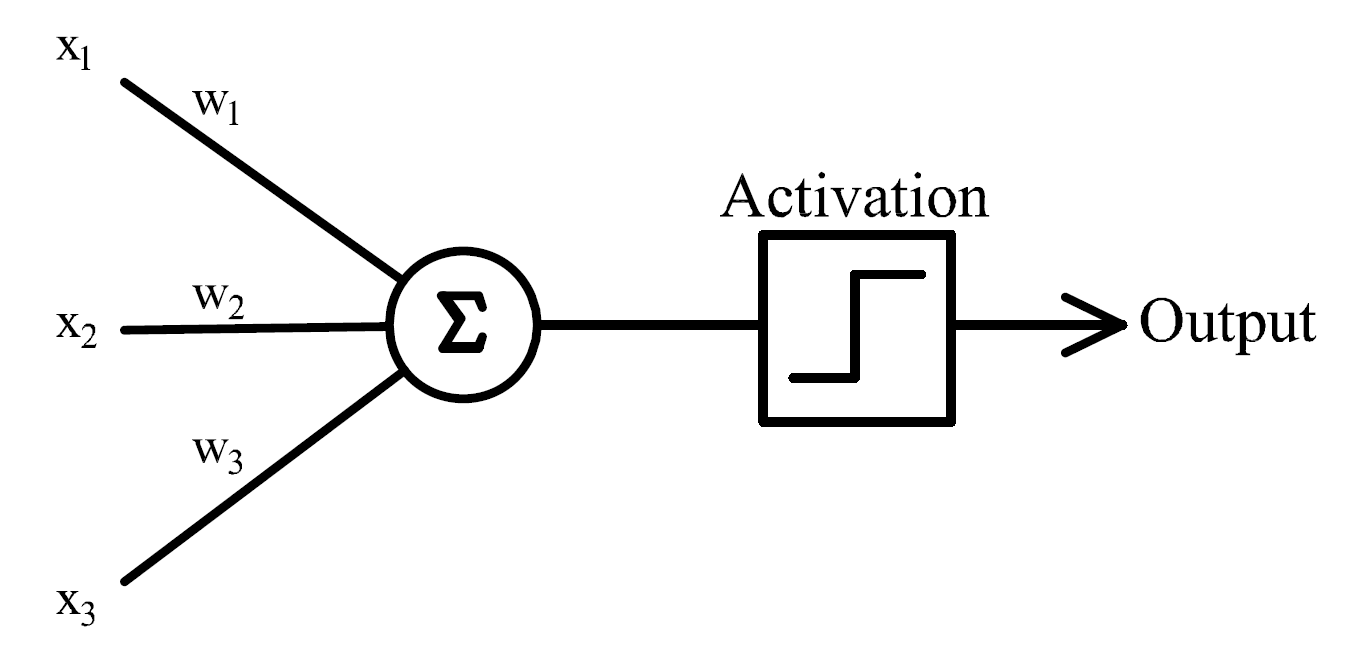
\includegraphics[scale=0.4]{../obrazy/fig:perceptron.png}
\caption{Perceptron przedstawiony na przykładzie składa się z dwóch warstw – warstwy wejściowej z trzema wartościami wejściowymi (\(x_1, x_2, x_3 \)) oraz warstwy wyjściowej.\label{fig:perceptron}}
\source{Opracowanie własne na podstawie \citet{rosenblatt1957}.}
\end{figure}

Przyjmuje on wektor \(\mathbf{x}\) binarnych wartości wejściowych \(x_1, \ldots, x_n \). Każda z tych wartości wejściowych jest przyjmowana z wagą \(w_1, \ldots, w_n \), będącą liczbą rzeczywistą. Owe parametry można w intuicyjny sposób przedstawić jako wpływ (mający wartość i kierunek) każdego z sygnałów wejściowych na sygnał wyjściowy. Ostatecznie ważona suma wartości wejściowych porównywana jest z wartoscią progową (\textit{threshold}), będącą kolejnym parametrem perceptronu. W przypadku, gdy ważona suma jest większa od wartości progowej, funkcja aktywacji zwraca wartość wyjściową 1, w przeciwnym wypadku zwraca 0. Równanie \ref{eq:perc_activation} zawiera formalną reprezentację funkcji aktywacji.

\begin{equation} \label{eq:perc_activation}
  output=\begin{cases}
    0& \text{jeśli $\sum_j$ $w_j$ $x_j$ $<$ threshold},\\
    1& \text{jeśli $\sum_j$ $w_j$ $x_j$ $\geq$ threshold}.
  \end{cases}
\end{equation}

Algorytm uczenia perceptronu w $T$ iteracjach dla $N$ obserwacji uczących i $M$ wag przedstawiony został w Algorytmie \ref{alg:perceptron}.

\begin{algorithm}
\caption{Algorytm uczenia perceptronu}\label{alg:perceptron}
  \begin{algorithmic}[1]
    \State Inicjalizacja losowych wag $W$
    \For{$t \in \{1,\dots,T\}$}
      \For{$i \in \{1,\dots,N\}$}
        \State {$E = y - \sigma(W_{t-1} \cdot \mathbf{x_i})$}
        \For{$j \in \{1,\dots,M\}$}
          \State {$W_j = W_j + \alpha \cdot E \cdot \sigma^\prime(W_j \cdot x) \cdot x_j$}
        \EndFor
      \EndFor
    \EndFor
  \end{algorithmic}
\end{algorithm}

\citet{widrow1960} przedstawili ADALINE - jednowarstwową sztuczną sieć neuronową (Rysunek \ref{fig:ADALINE}), która uczona była za pomocą szczególnego przypadku do dzisiaj wykorzystywanej metody optymalizacji opartej na gradiencie - \textit{stochastic gradient descent}.

\begin{figure}[h]
  \centering
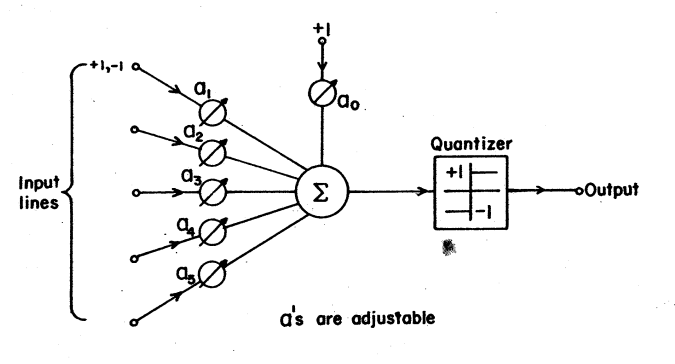
\includegraphics[scale=0.4]{../obrazy/fig:ADALINE.png}
\caption{Architektura ADALINE (\textit{Adaptive Linear Neuron}), która bazowała na projekcie sieci zaprezentowanym przez \citet{mcculloch1943}. Istotna różnica polega na dobraniu algorytmu optymalizacji wag. \label{fig:ADALINE}}
\source{Opracowanie własne na podstawie \citet{widrow1960}.}
\end{figure}

Jednym z pierwszych przykładów architektury, którą można uznać za wielowarstwową sieć neuronową jest zaprojektowany w pracach \citet{ivakhnenko1965}, \citet{ivakhnenko1967} oraz \citet{ivakhnenko1968} system będący reprezentantem rodziny metod GMDH (\textit{Group Method of Data Handling}). Jego charakterystycznymi cechami było wykorzystanie wielomianów Kolmogorova-Gabora jako funkcji aktywacji i użycie zbioru treningowego do uczenia i rozbudowywania kolejnych warstw sieci, by następnie przycinać je z wykorzystaniem zbioru walidacyjnego.

Pomimo obiecujących początków i optymizmu towarzyszącemu nowemu odkryciu, badania nad sztucznymi sieciami neuronowymi zostały w dużej części porzucone za sprawą publikacji \citet{minsky1969}. Nakreślili oni granice możliwości modeli liniowych (w tym perceptronu i jednowarstwowych sieci neuronowych) jako systemu uczącego się. W szczególności udowodnili, że z wykorzystaniem tego typu algorytmów nie da się odwzorować funkcji logicznej XOR. Ich odkrycie zakończyło pierwszy okres popularności sieci neuronowych, zwany cybernetyką.

Kolejna fala popularności sieci neuronowych została zapoczątkowana przez interdyscyplinarny ruch - koneksjonizm (\textit{connectionism}), określany również jako modele PDP (równoległego rozproszonego przetwarzania informacji). Wiele idei wywodzących się z cybernetyki zostało w tym okresie zaadaptowanych do badań nad charakterem poznania, por. \citet{touretzky1985}. Jedną z nich jest pomysł rozproszonej reprezentacji \citep{hinton1986}, opisywany także w pracy \citet{touretzky1985} jako inspirowany naturą i z niej się wywodzący. Przedstawia on założenie, że każdy sygnał wejściowy powinien być reprezentowany przez wiele cech systemu, a każda cecha powinna być włączona w tworzenie reprezentacji możliwie wielu sygnałów wejściowych. Wprowadzenie tej architektury było również odpowiedzią na krytykę koneksjonizmu, a jej wykorzystanie dowodem na to, że teorie wchodzące w skład tego paradygmatu pozwalają na stworzenie systemu zdolnego do rozwiązywania skomplikowanych problemów. Koncept rozproszonej reprezentacji pozostaje kluczowym komponentem konstruowanych obecnie sieci neuronowych, por. \citet{goodfellow2016}.

W tym okresie przedstawiono również inny koncept stosowany dotychczas - jednostki konwolucyjne (\textit{convolutional units}). Celem pracy \citet{fukushima1980} było zaproponowanie sztucznej sieci neuronowej, która mogłaby być wiernym modelem procesu rozpoznawania wzorów i kszałtów geometrycznych przez człowieka. Przedstawiono w niej model uczenia bez nadzoru, nazwany wówczas Neocognitron (będącą rozszerzeniem modelu Cognitron, zaproponowanego wcześniej przez Autora, por. \citet{fukushima1975}) i zastosowano architekturę, która jest protoplastą szeroko stosowanych sieci konwolucyjnych (używanych jednak obecnie głównie do rozwiązywania problemów ,,z nauczycielem''). Fukushima wprowadzał do modelu jako sygnał dwuwymiarową macierz, po której następujował szereg struktur składających się z pary warstw ukrytych odpowiadających komórkom niższego i wyższego rzędu (\textit{S-layer} oraz \textit{C-layer}). Schemat opisywanej architektury zaprezentowany został na Rysunku \ref{fig:neocognitron}. Istotnym z punktu widzenia \textit{deep learningu} i \textit{pattern recognition} było zastosowanie w niej warstw złożonych z jednostek konwolucyjnych, których pole receptywne było dwuwymiarową macierzą skokowo przesuwaną przez macierz wartości wejściowych (Rysunek \ref{fig:convolution}). Zwracane przez warstwy konwolucyjne macierze stanowiły wartości wejściowe dla warstw konwolucyjnych wyższego rzędu, operujących na wyższym poziomie abstrakcji. Każdy z elementów ostatniej warstwy tak skonstruowanej sieci neuronowej odpowiadał tylko na jeden rodzaj sygnału wejściowego. Owe zabiegi pozwoliły na skonstruowanie modelu, który byłby niewrażliwy na małe zmiany w kształcie, obrót lub translację sygnału wejściowego (Rysunek \ref{fig:distortion}). Należy jednak zwrócić uwagę na fakt, że ,,niewrażliwość'' na tego typu przekształcenia nie sprowadza się do takiego samego traktowania przekształcanego sygnału wejściowego przez pierwszą warstwę sieci. Sygnał wejściowy poddany na przykład translacji interpretowany jest przez inny zestaw neuronów niż pierwotny sygnał. Te same cechy tych sygnałów są jednak, ze względu na wykorzystanie jednostek konwolucyjnych, wykrywane niezależnie od ich położenia - mowa zatem raczej o równoważności interpretacji, a nie jej niezmienności w zależności od tego typu zmian w sygnale wejściowym.

\begin{figure}[h]
  \centering
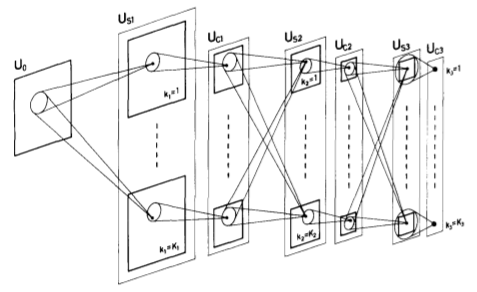
\includegraphics[scale=0.7]{../obrazy/fig:neocognitron.png}
\caption{Architektura modelu Neocognitron. W jej skład wchodzi warstwa wejściowa \(U_0\), po której następują trzy pary warstw ukrytych \(U_{Si} \) i \(U_{Ci} \) - odpowiednio niższego i wyższego rzędu.\label{fig:neocognitron}}
\source{\citet{fukushima1980}.}
\end{figure}

\begin{figure}[h]
  \centering
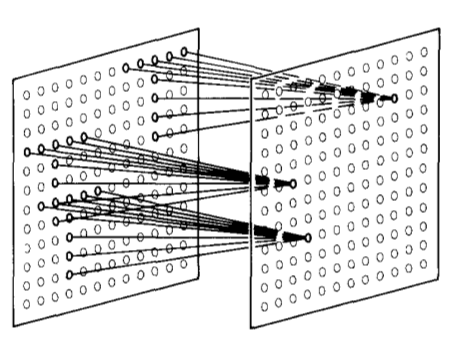
\includegraphics[scale=0.5]{../obrazy/fig:convolution.png}
\caption{Ilustracja połączeń dla przykładowych jednostek konwolucyjnych, zaproponowanych przez Fukushimę.\label{fig:convolution}}
\source{\citet{fukushima1980}.}
\end{figure}

\begin{figure}[h]
  \centering
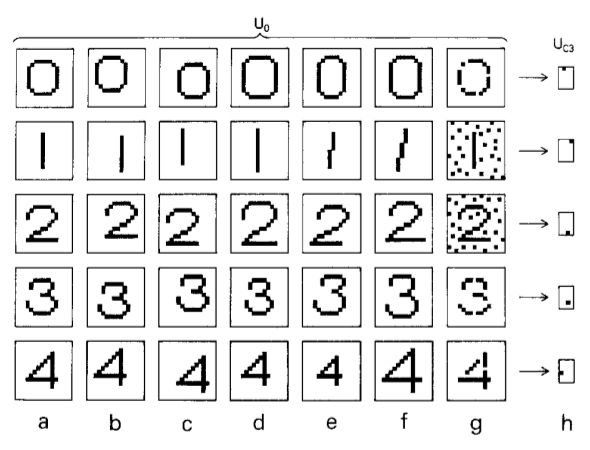
\includegraphics[scale=0.5]{../obrazy/fig:distortion.png}
\caption{Przykłady wartości wejściowych (b - g) będących pewną modyfikacją pierwotnego obrazu (a), dla których Neocognitron zwraca ten sam rezultat (h).\label{fig:distortion}}
\source{\citet{fukushima1980}.}
\end{figure}

Oprócz przełomu na polu nauk poznawczych, nastąpił również rozwój metod optymalizacyjnych. Praca \citet{rumelhart1986} dowiodła empirycznie skuteczność algorytmu propagacji wstecznej (\textit{backpropagation}) w przyspieszaniu procesu uczenia sieci neuronowych, co przyczyniło się do wzrostu popularności owej metody i pozwoliło na wykorzystywanie sieci neuronowych do szerszego zakresu problemów. Ta procedura optymalizacji, przedstawiona po raz pierwszy w pracy \citet{linnainmaa1970}, polegała na iteracyjnym korygowaniu wartości wag w sieciach neuronowych w celu minimalizacji wybranego kryterium błędu (Algorytm \ref{alg:backpropagation}), por. również \citet{hecht1988}. W pracy \citet{rumelhart1986} neurony warstw ukrytych, których stan lub zadanie nie zostało zawczasu ustalone, mogły reprezentować istotne cechy sygnału wejściowego. Możliwość wykrywania cech sygnału wejściowego bez ich wskazywania w sposób jawny, miała w znaczny sposób odróżniać przedstawiony system od sposobów uczenia skonstruowanych w erze cybernetyki. Potwierdzeniem tej tezy był fakt wygrania międzynarodowego konkursu predykcyjnego poprzez wykorzystanie modelu sieci neuronowych uczonego z użyciem algorytmu propagacji wstecznej \citep{wan1993}. W publikacji \citet{rumelhart1986} zaproponowano również pewną modyfikację do metody SGD - metodę pędu (\textit{momentum method}), która, inspirowana zjawiskiem fizycznym, miała zapobiec zbyt długiemu oscylowaniu wokół ekstremów funkcji celu w optymalizacji gradientowej.

\begin{algorithm}
\caption{Algorytm propagacji wstecznej}\label{alg:backpropagation}
  \begin{algorithmic}[1]
    \State Inicjalizacja losowych wag $W$
    \For{$t \in \{1,\dots,T\}$}
      \For{$e \in \{1,\dots,N\}$}
        \State Oblicz wartości wejściowe $in_i$ i wyjściowe $out_i$ każdego neuronu dla $x_i$
        \For{$(j,i)$ (wszystkich wag idąc wstecz)}
          \If{i jest neuronem warstwy wyjściowej}
            \State $ \Delta_i = (y_i-out_i) \cdot \sigma^\prime(in_i) $
          \Else
            \State $ \Delta_i = \sigma^\prime(in_i)\sum_{k}w_{i,k}\Delta_k $
          \EndIf
          \State $ W_{j,i} = W_{j,i}+\alpha \cdot {out_j} \cdot \Delta_i $
        \EndFor
      \EndFor
    \EndFor
  \end{algorithmic}
\end{algorithm}

Algorytm propagacji wstecznej, choć będący bardzo użytecznym narzędziem, nie spełnił pokładanych w nim nadziei i nie był rozwiazaniem wszystkich problemów tego typu modeli. Pomimo faktu, że w teorii pozwalał na uczenie głebokich sieci, wydawało się, że spektrum jego zastosowań mieści się tylko w zakresie płytkich architektur. Większość sieci, które były projektowane ograniczały się do kilku warstw ukrytych, jako że dodawanie kolejnych warstw nie przynosiło oczekiwanych rezultatów. W kolejnych latach zaproponowano wiele usprawnień w zakresie algorytmów optymalizujących proces uczenia. Oprócz uprzednio wspomnianej metody pędu, przedstawiono również metody polegające na ustaleniu osobnych szybkości uczenia (\textit{learning rate}) dla różnych sieci, por. \citet{jacobs1989}, a także \citet{almeida1990}. Uzasadnieniem tego zabiegu jest różnica w szybkości uczenia pomiędzy różnymi warstwami sieci, ale także pozwala on na dynamiczne zmniejszanie \textit{learning rate} w przypadku wag, w których następują częste zmiany kierunku gradientu. \citet{jacobs1989} zaproponował również połączenie tej metody z metodą pędu.
Osobnym wariantem propagacji wstecznej jest Rprop - metoda zaproponowana przez \citet{riedmiller1993}, jak również metody od niej pochodzące: iRprop+ \citep{igel2003} oraz RMSProp \citep{tieleman2012}. Istotą Rprop jest wykorzystywanie wyłącznie znaku gradientu przy estymowaniu modelu z wykorzystaniem całego zbioru danych (\textit{full-batch learning}) w celu zminimalizowania trudności z wyborem globalnej \textit{learning rate}. Krok uczenia jest zwiększany w przypadku, gdy znak gradientu pozostaje niezmienny, w przeciwnym wypadku zostaje zmniejszany. Optymalizacja z wykorzystaniem części zbioru danych (\textit{mini-batch learning}) opiera się na założeniu o uśrednieniu kierunku gradientu dla wielu partii zbioru danych. Założenie to nie jest spełnione w przypadku wykorzystania algorytmu Rprop i z tego powodu nie jest wskazane stosowanie tej metody w połączeniu z \textit{mini-batch learning}. Ulepszenie algorytmu Rprop - iRProp+ polega na sprawdzeniu dodatkowych warunków dotyczących zmiany funkcji błędu poza sprawdzeniem zmiany kierunku gradientu. W przypadku zmiany kierunku gradientu i poprawy funkcji celu (zmniejszenia błędu), nie następuje korekta wag. Z kolei rozwiązaniem problemu braku możliwości uczenia modelu z wykorzystaniem wielu partii zbioru danych jest wspomniana metoda RMSProp. Metodę Rprop można alternatywnie przedstawić jako wykorzystanie klasycznej metody gradientowej przy dodatkowym dzieleniu przez wartość gradientu w każdym kolejnym kroku.
Istotą RMSProp jest wprowadzenie ruchomej średniej kwadratu gradientu dla każdej z wag, tak, by w każdej kolejnej partii zbioru danych zamiast dzielenia przez wartość gradientu, dzielić przez jej pierwiastek kwadratowy (Równanie \ref{eq:rmsprop_ma}).

\begin{equation} \label{eq:rmsprop_ma}
  {MA}(w,t) = 0,9 \cdot {MA}(w, t-1) + 0,1 \cdot (\frac{\partial E}{\partial w}(t))^2
\end{equation}

Ówczesny obszar badań obejmował również prace nad mniej skomplikowanymi modelami sieci neuronowych, które miałyby wysoką zdolność uogólniania. Próbowano w ten sposób zapobiec przeuczaniu tego typu modeli, które ze względu na ich pojemność informacyjną jest dużym ryzykiem. Przykładem popularnego podejścia, które skupiało się na znalezieniu odpowiedniego balansu między wariancją, a obciążeniem modelu (\textit{bias-variance dillemma}) jest metoda \textit{weight decay} \citep{hanson1990}. Sprowadza się ona do ograniczania wartości wag za pomocą metod regularyzacji, w tym \textit{L1} lub \textit{L2}, podobnie jak ma to miejsce w modelach regresji. Ponieważ propagacja wsteczna jest szczególnym przypadkiem wielowymiarowych, nieliniowych metod regresyjnych, a wartości wejściowe są często skorelowane, nie są spełnione warunki potrzebne do uzyskania nieobciążonego estymatora o najmniejszej wariancji. Wtedy sztuczne obciążenie estymatora może zmniejszyć jego wariancję, poprawiając stabilność modelu.

Alernatywną metodą do osiągnięcia tego samego celu jest wykorzystanie podejścia bayesowskiego, por. \citet{nowlan1992}, \citet{hinton1993}, a także \citet{edwards1993}. Bayesowska interpretacja \textit{weight decay} polega na minimalizowaniu logarytmów prawdopodobieństwa - logarytmu prawdopodobieństwa a posteriori ($P(W|D)$) i logarytmu prawdopodobieństwa a priori ($P(W)$), które odpowiadają kosztowi (na przykład kwadratowej funkcji kosztu) i wyrażeniu regularyzującemu. Wartości wag \textit{a priori} mogą również zostać \textit{implicite} zawarte w dodatkowych karach \citep{mackay1992} lub poprzez użycie metod opartych na zbiorze walidacyjnym \citep{hastie1990}, kryterium informacyjnym Akaike \citep{akaike1974} lub oczekiwanym błędzie predykcji \citep{moody1994}. Do podobnych sposobów poprawy zdolności uogólniania sieci neuronowych zaliczyć można oparte na upraszczaniu architekury, jak sekwencyjne budowanie sieci warstwa po warstwie \citep{ivakhnenko1968}, przycinanie wartości wejściowych \citep{moody1991}, a także przycinanie wag \citep{lecun1989a}.

W 1989 roku stworzono sieć neuronową w oparciu o przedstawiony wcześniej model Neocognitron \citet{fukushima1980} i z wykorzystaniem algorytmu propagacji wstecznej, por. \citet{lecun1989b}. Do skonstruowania tego systemu użytu również jednostek konwolucyjnych, idei współdzielenia wag i zasilono go nowym konceptem - \textit{max pooling}. Współdzielenie wag (\textit{weight sharing}) opisane zostało w pracy \citet{rumelhart1986} dla problemu T-C i polegało na sterowaniu wieloma połączeniami jednym paramentrem wagi. W ten sposób nie tylko znacznie redukuje się liczbę potrzebnych parametrów w sieci, ale także opisuje się topologię przedstawionego zadania. Architektura omawianej sieci została przedstawiona na Rysunku \ref{fig:lecunmnist}. Składa się z trzech warstw ukrytych (H1, H2, H3). Połączenia pomiędzy warstwą H1 a H2 zostały sztucznie ograniczone. Warstwa H1 składa się z 12 grup 64 jednostek, gdzie każda z nich jest niezależnym zbiorem map cech o wymiarze 8x8. Każda jednostka w pierwszej warstwie przyjmuje wartość wejściową w postaci macierzy 5x5 ze źródłowego obrazu. Ponieważ z dużą pewnością można stwierdzić, że cechy istotne w jednej części obrazu będą również istotne w innych częściach obrazu, zastosowano w tej warstwie technikę \textit{weight sharing}. Zatem każda jednostka ma 26 wag, gdzie 25 jest współdzielone z resztą grupy, a 26, \textit{bias}, jest dla niej unikalna. W efekcie warstwa H1 składa się z $8\cdot8\cdot12=768$ jednostek, $768\cdot26=19968$ połączeń, ale jedynie $768+26\cdot25=1068$  parametrów. Podobna logika zastosowana została w warstwie H2, podczas gdy warstwa H3 składa się z 30 jednostek. w pełni połączonych z warstwą H2. Uczenie przyspieszono za pomocą procesorów graficznych, które okazały się istotnym komponentem w tym podejściu. Ponadto, publikacja ta wprowadziła również zbiór danych \textit{MNIST}, który do dzisiaj jest wykorzystywany jako poziom porównawczy dla wielu architektur sieci neuronowych. W przeciwieństwie do wielu poprzednich eksperymentów, w tej pracy wartością wejściową do modelu były surowe obrazy zamiast przygotowanych wektorów, co miało zademonstrować możliwość radzenia sobie z nieprzetworzonymi danymi przez tego typu systemy.

\begin{figure}[h]
  \centering
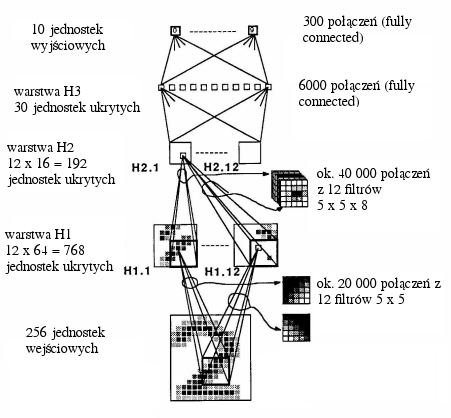
\includegraphics[scale=0.6]{../obrazy/fig:lecunmnist.png}
\caption{Model wykorzystany przez \citet{lecun1989b} do problemu identyfikacji kodów pocztowych, który jest jednym z pierwszych przykładów wykorzystania konwolucyjnych sieci neuronowych na szeroką skalę. \label{fig:lecunmnist}}
\source{\citet{lecun1989b}.}
\end{figure}

Istotne spostrzeżenie dotyczące sieci neuronowych zostało przedstawione w pracy \citet{hochreiter1991}. Wyjaśnił, dlaczego głębokie sieci neuronowe są trudne do uczenia z wykorzystaniem propagacji wstecznej (na co wcześniej wskazywały wyniki eksperymentów). Znaleziona przez niego przyczyna określona została później problemem znikającego i eksplodującego gradientu (\textit{vanishing gradients, exploding gradients}). W przypadku standardowych funkcji aktywacji, propagowany wstecz błąd w tempie wykładniczo zależnym od liczby warstw maleje bądź rośnie. Z biegiem czasu przedstawiono liczne podejścia do radzenia sobie z tym problemem, takie jak wstępne uczenie bez nadzoru (i w efekcie kompresja sygnału wejściowego), wykorzystanie procesorów graficznych, optymalizację bez wykorzystania Hesjanów lub całkowite uniknięcie stosowania metod optymalizacji opartych na gradiencie.

Prace nad Neocognitronem \citep{fukushima1980}, jak również wcześniejsze prace \citep{ivakhnenko1968} były inspiracją do stworzenia innego systemu uczącego się - Cresceptron, por. \citet{weng1992}, który dostosowuje swoją architekturę podczas uczenia. Cresceptron wykorzystuje technikę zwaną \textit{max pooling}, gdzie w jednostce macierz wejściowa zostaje zastąpiona przez jej maksymalną wartość. (\textit{Max pooling} oraz \textit{average pooling} zostały zaprezentowane zostały na rysunku \ref{fig:pooling}). Konwolucyjne sieci neuronowe, które wykorzystują tę technikę i uczone są za pomocą propagacji wstecznej zostały popularnym wyborem w późniejszych zastosowaniach i były częścią wielu kolejnych systemów uczących się.

\begin{figure}[h]
  \centering
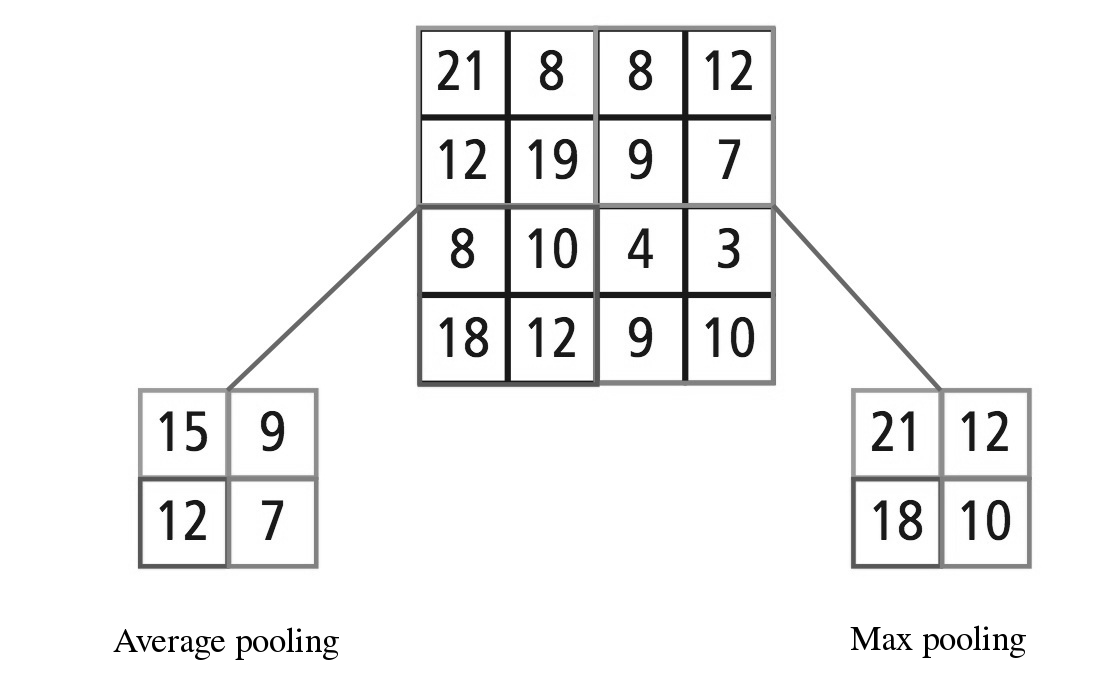
\includegraphics[scale=0.3]{../obrazy/fig:pooling.png}
\caption{Macierze wejściowa partycjonowana jest na skończoną liczbę mniejszych macierzy. \textit{Average pooling} przekształca każdą z tych macierzy w liczbę będącą średnią jej wartościa, podczas gdy \textit{max pooling} przekształca je w liczbę będącą maksymalną jej wartością. \label{fig:pooling}}
\source{Opracowanie własne.}
\end{figure}

Ruch koneksjonizmu utrzymywał zainteresowanie środowisk naukowych i biznesowych tylko do połowy lat 90. Nieproporcjonalne oczekiwania co do możliwości sztucznych sieci neuronowych oraz pojawienie się innych, bardziej obiecujących metod (jak maszyny wektorów nośnych) sprawiły, że inwestorzy wycofali swoje wsparcie. Na przełomie wieków istotne publikacje zostały przedstawione na polu rekurencyjnych sieci neuronowych, por. \citet{schmidhuber1997}, \citet{schuster1997} i \citet{graves2005}.

Aktualne zainteresowanie głębokimi sieciami neuronowymi zostało zapoczątkowane jako skutek badań nad modelami o skomplikowanej architekturze, por. \citet{hinton2006a}, \citet{hinton2006b}, a także \citet{bengio2007a}. Wtedy też tego typu architektury sieci neuronowych otrzymały określenie \textit{głębokich}. Miało na celu podkreślenie faktu wykorzystywania wielu ukrytych warstw i wstępnego trenowania sieci z wykorzystaniem technik uczenia bez nadzoru, co dotychczas nie było często eksplorowanym kierunkiem badań z powodu niedostatecznej mocy obliczeniowej. Istotność tych cech w sieciach neuronowych jest podkreślana w pracach \citet{bengio2007b} i \citet{bengio2011}.
W tym okresie przedstawiono również \textit{deep belief networks}, sieci neuronowe będące stosem \textit{Restricted Boltzmann Machines}, które z kolei zostały zaprezentowane w pracy \citet{smolensky1986} i są pewnym rozwinięciem klasycznych \textit{Boltzmann Machines}, por. \citet{hinton1986}. Algorytmy te znalazły od tego czasu zastosowanie w zagadnieniach takich jak redukcja wymiarów, klasyfikacja, silniki rekomendacyjne, \textit{feature learning} i \textit{topic modelling}. Istotą działania tych architektur jest pomysł, by każda kolejna warstwa przyjmowała reprezentację wzorów i cech z wcześniejszej warstwy i uczyła się ją przetwarzać bez nadzoru. Również w 2006 roku dokonana została istotna poprawa wyniku na omówionym zbiorze MNIST przez \citet{ranzato2006}, którzy osiągnęli błąd predykcji na poziomie 0,39\% bez wykorzystania uczenia wstępnego bez nadzoru. W tym okresie rozpoczęto korzystanie z procesorów graficznych w celu przyspieszenia uczenia zarówno sieci neuronowych \citep{oh2004}, jak i sieci konwolucyjnych \citep{chellapilla2006} - osiągnięto odpowiednio około 20 razy lepsze i około 4 razy lepsze czasy w porównaniu do wykorzystania wyłącznie jednostek centralnych.
W 2007 roku, propagacja wsteczna została po raz pierwszy wykorzystana do uczenia opartej na Neocognitronie i Cresceptronie sieci neuronowej, por. \citet{ranzato2007}. Konwolucyjne sieci neuronowe, wykorzystujące max-pooling i propagację wsteczną okazały się niezbędną częścią późniejszych architektur, które wygrywały międzynarodowe konkursy w rozpoznawaniu obrazu. Jednym z pierwszych sukcesów sieci konwolucyjnych na arenie światowej było wykorzystanie ich jako części systemu, który miał wyróżniać istotne regiony w nagraniach z kamer przemysłowych (\citet{jain2009} oraz \citet{yang2009}).

Ważnym sygnałem o rosnącej roli procesorów graficznych okazała się praca \citet{ciresan2010}. Model w niej przedstawiony nie zawierał żadnych przełomowych pomysłów z punktu widzenia architektury (co więcej, nie korzystał z uczenia wstępnego, ani jednostek konwolucyjnych), był jednak uczony z wykorzystaniem implementacji propagacji wstecznej na procesorach graficznych, która pozwoliła przyspieszyć cały proces 50-krotnie. Rok później, w publikacji \citet{ciresan2011a} zaprezentowano implementację uczenia sieci konwolucyjnych z max-poolingiem z wykorzystaniem GPU. Wtedy także dokonano przełomowego osiągnięcia w zakresie rozpoznawania obrazu, pokonując ludzkie zdolności poznawcze w tym zakresie podczas konkursu w rozpoznawaniu znaków drogowych, por. \citet{ciresan2011b}. Osiągnięty błąd predykcji 0,56\% okazał się dwukrotnie lepszy od błędu ludzkiego, trzykrotnie lepszy od kolejnej sieci neuronowej i sześciokrotnie lepszy od systemu nie opartego na sieciach neuronowych. Podobnego rodzaju architektura osiągnęła również najlepszy do tego czasu wynik w klasyfikacji obrazów ze zbioru danych MNIST
(0,2\%), co również było lepszym rezultatem od błędu predykcji przeciętnego człowieka.
Kolejnym osiągnięciem było uzyskanie pierwszego miejsca w problemie klasyfikacji na zbiorze danych ImageNet przez architekturę zaproponowaną przez \citet{krizhevsky2012}, bazującą na przedstawionych wcześniej modelach konwolucyjnych (w przypadku tego zbioru danych wartością wejściową były obrazy o rozmiarach 256x256 pikseli, w przeciwieństwie do znacznie mniejszych obrazów znaków drogowych - 48x48 pikseli).

Głębokie sieci neuronowe osiagały bardzo obiecujące wyniki w problemach klasyfikacji obrazów, jednak prawdopodobnie największe nadzieje są wiązane z rozpoznawaniem obiektów na obrazie, co mogłoby okazać się bardzo przydatne w intepretowaniu rezultatów badań medycznych jak zdjęcia wykonywane w celu diagnozowania chorób nowotworowych. Systemem, który wygrał konkurs dotyczący tych zagadnień (ICPR 2012 Contest on Mitosis Detection in Breast Cancer Historical Images, 2012) była sieć neuronowa stworzona przez \citet{ciresan2013}. Innym rodzajem problemu, który skutecznie można rozwiazań z wykorzystaniem tego typu modeli jest zagadnienie segmentacji pikseli na obrazach \citep{ciresan2012}.

Sztuczne sieci neuronowe znalazły dotychczas zastosowanie w problemach uczeniach z nadzorem, bez nadzoru, jak również w \textit{reinforcement learning}. Najważniejszymi kwestiami do zaadresowania w najbliższej przyszłości są te związane z podejściem do ich konstruowania. Należy odpowiedzieć na pytanie, jak sprawić, by systemy o wciąż wąskich obszarach specjalizacji, były zdolne do większego uogólniania. W przypadku rozpoznawania elementów na obrazach należy wzorować się na procesie poznawczym człowieka, który aktywnie wyszukuje wzorów na obrazie i zwraca uwagę na istotne kwestie. W tym wypadku warto również mieć na uwadze takie aspekty, jak samo etykietowanie danych, które jest procesem silnie humanocentrycznym, co poruszone zostało także w pracy \citet{misra2016}.

\clearpage

\subsection{Cloud computing}

\noindent
W tym rozdziale omówiony zostanie paradygmat przetwarzania danych w chmurze. Przedstawione zostaną jego kluczowe cechy, wymagania stawiane dostawcom i definicje często spotykanych pojęć. Następnie opiszemy najpopularniejsze modele świadczonych usług, modele implementacji i rozwiązania technologiczne leżące u podstaw opisywanego paradygmatu, by finalnie przejść do aspektów ekonomicznych i przybliżenia rynku \textit{cloud computingu} wraz z opisem największych dostawców.

\subsubsection{Definicje, kluczowe charakterystyki}

\noindent
Przetwarzanie danych w chmurze definiowane jest w pracach \citet{buyya2009} oraz \citet{calheiros2010} jako ,,rodzaj równoległego i rozproszonego systemu, składającego się z licznych, połączonych ze sobą i wirtualizowanych serwerów, która są dynamicznie przydzielane na podstawie ustaleń pomiędzy dostawcą a konsumentami, dokonanych za pośrednictwem dedykowanego serwisu''. Innymi słowy, w tym modelu pamięć, moc obliczeniowa znajdują się ,,w chmurze'', która jest zbiorem centrów danych (\textit{data centers}), posiadanych oraz utrzymywanych przez zewnętrzny podmiot. Konsumenci otrzymują dostęp do owej infrastruktury lub serwisów na niej bazujących przez wystosowanie żądania odwzorowującego ich aktualne potrzeby na tego typu usługi, bez wymagania rezerwacji z dużym wyprzedzeniem czasowym i znacznego nakładu kapitału (\textit{pay-as-you go model}).

To podejście, odnoszące się do świadczenia usług w zakresie dostarczania infrastruktury, mocy obliczeniowej lub aplikacji za pośrednictwem Internetu, stało się jednym z głównych paradygmatów w tej dziedzinie nauki i biznesu. Efektem tego optymizmu jest wizja dostarczania mocy obliczeniowej jako kolejnego rodzaju powszechnie dostępnego medium. Ma ono zaspokajać, ze stosunkowo niewielkim opóźnieniem, rosnące w erze digitalizacji zapotrzebowanie na jednostki będące w stanie wykonywać skomplikowane obliczenia. Leonard Kleinrock, naukowiec, który wniósł istotny wkład w budowę Internetu, twierdził w 1969 jako główny inżynier projektu ARPANET, że: ,,W chwili obecnej, sieci komputerowe są wciąż we wczesnym okresie rozwoju, jednakże wraz z ich dojrzewaniem obserwować będziemy rozpowszechnienie narzędzi komputerowych (\textit{computer utilities}), które jak obecnie elektryczność lub sieci telefoniczne, będą służyć gospodarstwom domowym i przedsiębiorstwom w całym kraju''  \citep{kleinrock2005}. Kleinrock skutecznie przewidział nie tylko mającą nadejść powszechność połączenia internetowego, lecz również możliwość wynajmowania maszyn wirtualnych w sposób zdalny, z natychmiastowym skutkiem, w zależności od aktualnego popytu - tak jak ma to miejsce przypadku każdego innego rodzaju powszechnie dostępnego medium. Również Nicholas Carr porównuje potencjalne konsekwencje nadchodzącej zmiany do tworzenia sieci elektrycznej na początku XX w., por. \citet{carr2008}. Kontynuując tę analogię, opłaty za tego typu usługę naliczane są tylko w wypadku, gdy konsument korzystał z dostępnych mu zasobów. Ponadto, podejście to eliminiuje konieczność utrzymywania własnej infrastruktury informatycznej - rewolucja w szczególności dotyczy sposobu projektowania rozwiązań technologicznych w przedsiębiorstwach, które dotychczas w tej materii opierały się na założeniu pełnej lub częściowej samodzielności centrów danych. Istotność tego typu serwisów podkreśla w swojej pracy również Armburst \citep{armburst2010} określając je jako długo wyczekiwane marzenie dostarczenia przetwarzania danych jako szeroko dostępnego medium, które będzie napędzać transformację przemysłu technologii informacyjnych, czyniąc jednocześnie udostępnianie oprogramowania coraz atrakcyjniejszym rodzajem świadczonych usług.

Oprócz korzyści strukturalnych i biznesowych, ekonomia skali towarzysząca tego typu przedsiewzięciom wpływa na zmniejszenie śladu ekologicznego centrów danych, por. \citet{oecd2014}. Odbywa się to zarówno poprzez zmniejszanie zjawiska określanego jako nadmiernie zaopatrywanie się w zasoby (\textit{over-provisioning}), jak również implementowanie efektywniejszych sposobów przetwarzania danych i tworzenia dedykowanych rozwiązań architektonicznych i instalacyjnych, takich jak systemy chłodzenia. Należy jednak również zwrócić szczególną uwagę na potencjalne zagrożenia związane z wzrastającą popularnością tego typu technologii takich jak bezpieczeństwa i prywatności danych. Zostaną one omówione w późniejszej części rozdziału.

Aby wprowadzić pewne terminy i usystematyzować zbiór pojęć wykorzystywany w niniejszej pracy, oparto się na zestawie rekomendacji wydanym przez Państwowy Instytut Norm i Technologii Stanów Zjednoczonych \citep{mell2011}. Określa on \textit{cloud computing} jako model stworzony w celu umożliwienia wszechobecnego, wygodnego, dostępnego na żądanie, współdzielonego zbioru konfigurowalnych zasobów komputerowych, które mogą zostać natychmiastowo dostarczone przy niewielkim wysiłku zarządzającego i minimalnym stopniu interakcji. Infrastruktura rozwiązań pozwalających na przetwarzanie danych w chmurze jest zestawieniem sprzętu komputerowego oraz oprogramowania, które można opisać jako warstwę fizyczną (sprzęt komputerowy: serwery, dyski twarde i komponenty sieciowe) i warstwę abstrakcyjną (oprogramowanie dostępne na warstwie fizycznej). Model ten cechować musi pięć kluczowych charakterystyk, wyróżnione również są trzy modele świadczonych usług i cztery modele implementacji.

\noindent
Kluczowe charakterystyki:
\begin{itemize}
\item samoobsługowość oraz dostępność na żądanie (\textit{on-demand self-service}) -- klient może jednostronnie wynajmować jednostki obliczeniowe, również w sposób zautomatyzowany,
\item szerokopasmowy dostęp sieciowy (\textit{broad network access}) -- oferowane usługi dostępne są za pośrednictwem sieci, dostęp do nich można uzyskać przez standardowe mechanizmy, z wykorzystaniem zróżnicowanych platform (takich jak laptopy, komputery osobiste, telefony komórkowe czy tablety),
\item błyskawiczna elastyczność (\textit{rapid elasticity}) -- zasoby mogą być w sposób elastyczny rezerwowane i zwalniane, również automatycznie. Z perspektywy konsumenta oferowane zasoby wydają się być nieograniczone,
\item mierzalność usług (\textit{measured service}) -- systemy w sposób automatyczny kontrolują i optymalizują wykorzystanie zasobów dostosowując się do pewnej, uprzednio ustalonej miary (typowo stawki określanej jako płać i korzystaj (\textit{pay-per-use}). Jednocześnie musi być zapewniona pełna transparentność zarówno dla dostawcy usług, jak i konsumenta.
\end{itemize}

\noindent
Modele świadczonych usług :
\begin{itemize}
\item Oprogramowanie jako usługa (\textit{Software as a Service, SaaS}) -- konsument otrzymuje gotowe oprogramowanie, aplikacje, działające w infrastrukturze chmurowej. Do tego typu rozwiązań włącza się różnego rodzaju aplikacje stworzone na potrzeby konkretnych procesów i celów biznesowych. Są one dostępne z różnych rodzajów klientów i urządzeń. Jako przykład tego typu usług zaliczyć można zarówno aplikacje e-mailowe skierowane do odbiorców biznesowych, jak również zintegrowane systemy zarządzania relacjami z klientem. Konsument nie zarządza leżącą u podstaw aplikacji infrastrukturą (w tym siecią, serwerami, systemami operacyjnymi, pamięcią),
\item Platforma jako usługa (\textit{Platform as a Service, PaaS}) -- konsument otrzymuje możliwość wdrażania do infrastruktury chmurowej aplikacji stworzonych z wykorzystaniem wspieranych przez dostawcę języków programowania, bibliotek i narzędzi. Dostawcy tego typu usług posługują się i udostępniają dedykowane interfejsy programistyczne aplikacji (\textit{Application Programming Interface (API)}). Również w tym wypadku konsument nie zarządza infrastrukturą technologiczną,
\item Infrastruktura jako usługa (\textit{Infrastructure as a Service, IaaS}) -- konsument otrzymuje możliwość zarządzania sieciami, pamięcią, jednostkami obliczeniowymi i innymi fundamentalnymi zasobami, mogąc jednocześnie wdrażać i uruchamiać dowolne oprogramowanie, w tym rówież systemy operacyjne i aplikacje. Pozwala to konsumentowi na dużą elastyczność w zaspokajaniu swoich potrzeb informatycznych, nie ma jednak wciąż dostępu do fizycznej infrastruktury.
\end{itemize}

Schemat modeli usług świadczonych w chmurze wraz z porównaniem do tradycyjnych systemów IT zaprezentowany został również na Rysunku \ref{fig:cloudarch}.

\begin{figure}[h]
  \centering
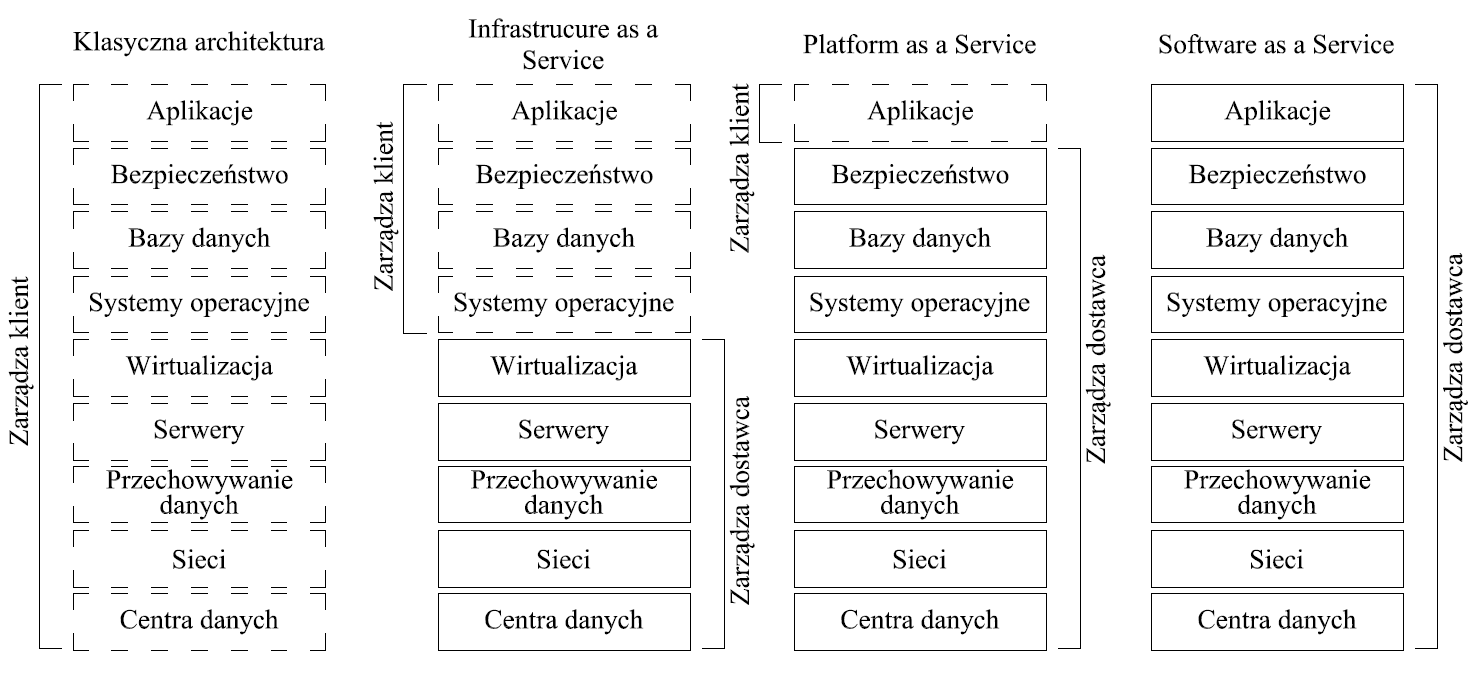
\includegraphics[width=\textwidth, keepaspectratio]{../obrazy/fig:cloudarch.png}
\caption{Stopień ingerencji w oferowane zasoby jest największy w przypadku platformy IaaS, podczas gdy rozwiązania SaaS pozwala użytkownikowi na minimalną inwestycję czasową w zarządzanie infrastrukturą \label{fig:cloudarch}}
\source{Opracowanie własne na podstawie ,,Cloud Computing - les différents modèles de service'' (PhFabre, Wikimedia Commons).}
\end{figure}

Należy jednak mieć na uwadze, że rozgraniczenie pomiędzy modelem \textit{IaaS} i \textit{PaaS} nie jest aż tak wyraźne jak w przypadku modelu \textit{SaaS}. W niektórych publikacjach \citep{armburst2010} są one traktowane jako grupa rozwiązań, które podzielają więcej podobieństw niż różnic.

\noindent
Modele implementacji:
\begin{itemize}
\item Prywatna chmura (\textit{Private Cloud}) -- infrastruktura zostaje udostępniona na wyłączność dla pojedynczego podmiotu lub organizacji. Może być posiadana i zarządzana przez tę organizację, podmiot trzeci lub dowolną ich kombinację. Może istnieć na terenie dostawcy usług lub poza nim,
\item Zbiorowa chmura (\textit{Community cloud}) -- infrastruktura udostępniona zostaje na wyłączność dla pewnej zbiorowości podmiotów, która mają wspólne cele. Może być posiadana i zarządzana przez jedną lub wiecej z organizacji należących do owej zbiorowości, podmiotu trzeciego lub dowolnej ich kombinacji. Może istnieć na terenie dostawcy usług lub poza nim,
\item Publiczna chmura (\textit{Public cloud}) -- infrastruktura udostępniona dla wszystkich użytkowników. Może być posiadana i zarządzana przez przedsiebiorstwo prywatne lub publiczne, placówkę akademicką lub dowolną ich kombinację. Musi istnieć na terenie dostawcy usług,
\item Hybrydowa chmura (\textit{Hybrid cloud}) -- infrastruktura jest połączeniem dowolnych dwóch lub więcej infrastruktur chmurowych, które pozostają odrębnymi bytami, lecz są związane rozwiązaniami technologicznymi. W przypadku połączenia prywatnej i publicznej chmury pozwala to na utrzymywanie dedykowanej infrastruktury, stanowiącej rdzeń systemu informatycznego przedsiębiorstwa, która w razie wyjątkowego obciążenia systemu lub awarii może zostać wspomagana zasobami pochodzącymi z chmury publicznej, por. \citet{antonopoulos2010}.
\end{itemize}

Ponieważ wiele prywatnych centrów danych korzysta z terminu ,,przetwarzania w chmurze'' w celu opisania swojego modelu biznesowego i przejaskrawienia potencjalnych korzyści, \citet{armburst2010} silnie podkreślają różnicę pomiędzy stosowanymi przez takich dostawców rozwiązaniami, a infrastrukturą posiadającą wszystkie wskazane cechy. Uargumentowane jest to faktem, że ekonomia skali i możliwość błyskawicznego dostosowywania się do zmian w popycie jest w przypadku tego przedsięwzięcia kluczowym czynnikiem, fundamentalnym dla jego opłacalności. Małej i średniej wielkości centra danych (nie posiadające setek tysięcy-milionów serwerów) nie mogą oferować swoim klientom atrakcyjniejszych cen, ponieważ czerpią tylko z podzbioru wymienionych wcześniej możliwości. Ponadto, jak twierdzi \defcitealias{mustafa2015}{Mustafa (2015)}\citetalias{mustafa2015}, paradygmat \textit{cloud computingu} jest w swojej naturze skierowany na potrzeby rynku, podczas gdy klasyczna architektura jest systemocentryczna i nie daje dostawcy bodźców do traktowania wszystkich zgłoszeń z równą wagą. Z wymienionych powodów prywatny model chmury często nie jest przywoływany w debatach nad tego typu rozwiązaniami.

Na tym etapie warto również przywołać pokrewne technologie, takie jak \textit{grid computing} oraz \textit{utility computing}, por. \citet{zhang2010}. \textit{Grid computing}, zwany również przetwarzaniem sieciowym jest paradygmatem rozproszonego przetwarzania danych, który koordynuje zasoby znajdujące się w jednej sieci, by osiągnąć jeden ustalony cel w przetwarzaniu. To rozwiązanie ma swoje korzenie w środowisku naukowym, gdzie wykonywane obliczenia potrzebowały dużej ilości zasobów. Różnica pomiędzy nim a przetwarzaniem w chmurze polega na stopniu wykorzystywania technologii wirtualizacji na wielu poziomach (sprzętowym i aplikacyjnym). Druga z wymienionych technologii, \textit{utility computing}, reprezentuje model dostarczania zasobów na żądanie i fakturowaniu klientów na podstawie ich wykorzystania zamiast stałej stawki. Przetwarzanie w chmurze może być rozpatrywane jako pewnego rodzaju realizacja \textit{utility computingu}. Adaptuje ona schemat ustalania stawek ze względów czysto ekonomicznych.

\subsubsection{Wirtualizacja i zarządzanie zasobami}

\noindent
U podstaw przedstawianej infrastruktury leżą dwie technologie: wirtualizacja oraz zarządzanie zasobami \citep{mustafa2015}. Techniki wirtualizacyjne wykorzystywane są w celu zapewnienia elastycznego i dynamicznego przydzielania mocy obliczeniowej, podczas gdy proces zarządzanie zasobami odpowiada za ich dostarczanie i nadzór nad nimi. Dzieje się to poprzez dzielenie jednej fizycznej maszyny na wiele logicznych systemów operacyjnych z wykorzystaniem hipernadzorcy (\textit{hypervisor}), który emuluje leżący u podstaw model sprzętowy i odpowiada za inicjalizację i nadzorowanie pracy wielu systemów operacyjnych. Rysunek \ref{fig:vm}. przedstawia działanie takiego typu architektury i porównuje go do tradycyjnego podejścia. Wirtualizowany serwer powszechnie nazywany jest maszyną wirtualną (\textit{Virtual Machine, VM}). Cykl życia maszyny wirtualnej obejmuje sześć faz: tworzenie, zawieszenie, wznowienie, zapisanie, migrację oraz niszczenie.

Wirtualizacja po raz pierwszy została wykorzystana na wielką skalę przez IBM w latach 1960 przy systemach klas komputerów określanych jako komputery głównego szeregu (\textit{mainframe systems}). Środowiska wirtualne i systemy operacyjne używane na tych komputerach pozwalały na uruchamianie wielu aplikacji i procesów dla wielu użytkowników jednocześnie i utrzymanie wysokiego poziomu automatyzacji przydzielania zadań. Robert P. Goldberg w 1974 roku opisał potrzebę wykorzystywania maszyn wirtualnych w następujący sposób: ,,Systemy maszyn wirtualnych były oryginalnie zbudowane by naprawić pewne wady architektur trzeciej generacji i wieloprogramowych systemów operacyjnych (\textit{multiprogramming operating systems}, takich jak OS/360'' \citep{goldberg1974}. W latach 1980 i 1990 dominującym podejściem do przetwarzania danych były systemy rozproszeone, aplikacje klient-serwer oraz tanie serwery x86. Osiagnięcia technologiczne ostatnich lat doprowadziły jednak do znacznego wzrostu wydajności stosowania tego typu rozwiązań i wykorzystania wielordzeniowych procesorów na szeroką skalę. Opracowane niedawno, popularne architektury sprzętowe, takie jak rodzina architektur procesorów Intel X86 czy AMD-V silnie czerpią z tego modelu (przykładem mogą również być takie implementacje jak VMware, Xen czy KVM, por. \citet{shroff2010}). Powrót do tego podejścia argumentowany jest także oszczędnością energii \citep{ward2013}, znacznie większą stabilnością tak zaprojektowanego systemu, a w przypadku przedsiębiorstw oferujących usługi przetwarzania w chmurze również możliwością dostosowywania się do błyskawicznie zmieniających się potrzeb konsumentów. Przykładowo w przypadku awarii jednej z maszyn, wszystkie wykonywane przez nią zadania automatycznie zostają migrowane na jedną lub wiele pozostałych jednostek. Ponadto, dostawcy muszą mieć pewność, że są wystarczająco elastyczni, by w czasie rzeczywistym zaspokajać popyt na różne rodzaje jednostek, izolując jednocześnie w wymaganym stopniu użytkowników od fizycznej infrastruktury. To podejście do zarządzania zasobami, ich stałe monitorowanie i możliwość automatycznego reagowania na awaryjne sytuacje muszą być zapewnione w przypadku środowiska \textit{cloud computingowego} i są jego inherentną częścią.

\begin{figure}[h]
  \centering
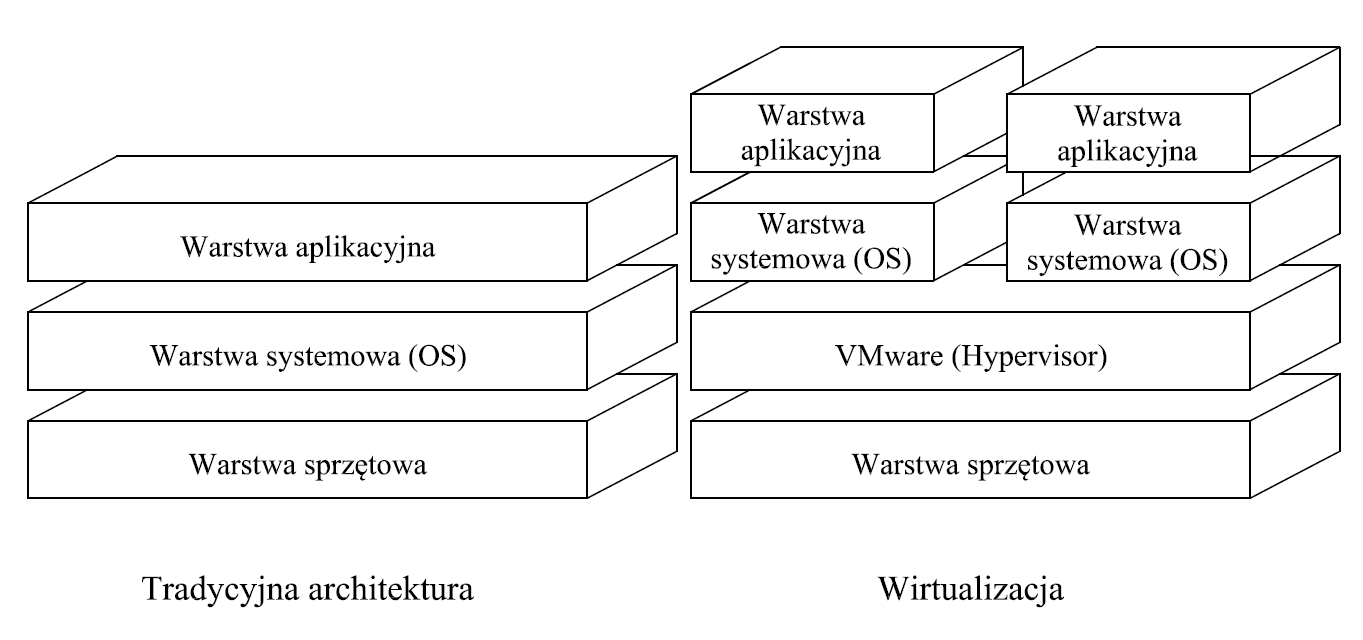
\includegraphics[scale=0.4]{../obrazy/fig:vm.png}
\caption{Wirtualizacja pozwala na uruchomienie licznych maszyn wirtualnych na jednej maszynie fizycznej z wykorzystaniem hipernadzorcy (w tym wypadku \textit{VMware}) \label{fig:vm}}
\source{Opracowanie własne na podstawie ,,OS-level vs Hardware-level virtualization'' (RicoRico, Wikimedia Commons).}
\end{figure}

Technologia wirtualizacji musi jednak zmierzyć się z pewnymi wyzwaniami. Architektura x86 nie była pierwotnie tworzona jako platforma dedykowana tym rozwiązaniom. Mechanizmy, które pozwalają na tworzenie maszyn wirtualnych na tego typu architekturze wymagają zmodyfikowanego systemu operacyjnego lub używają dodatkowego zestawu instrukcji, dostarczonego przez nowoczesne procesory. Z tego powodu wykorzystywanie wirtualizacji wiąże się z pewnym spadkiem wydajności. Choć według \citet{menon2005} został on w ostatnich latach zminimalizowany, wirtualne maszyny wciąż dostarczają tylko ułamek wydajności równoważnej fizycznej maszyny. Niektóre rodzaje hipernadzorców pozwalają na dostarczenie niemal natywnej wydajności procesora, jednak sedno problemu leży w wydajności procesów wejścia/wyjścia (\textit{input/output (I/O)}), którego spowolnienie może osiągać nawet 88\% w porównaniu do maszyny fizycznej. Ponadto, należy skupić się także na minimalizowaniu strat w przypadku uruchamianie wielu maszyn wirtualnych na jednym rdzeniu procesora. Ponieważ w danym momencie na jednym procesorze może być aktywna tylko jedna maszyna wirtualna, pozostałe z nich pozostają bezczynne i nie mogą odpowiadać na aktywność \textit{I/O}.

\subsubsection{Aspekty ekonomiczne}

\noindent
Przetwarzanie w chmurze stało się jedną z najszybciej rozwijających się gałęzi technologii informacyjnych. W 2009 r. sprzedaż w usługach chmurowych osiągnęła 56 miliardów dolarów \citep{smith2009}, podczas gdy Merryl Lynch przewidywał wzrost wartości rynku do 160 miliardów w 2011. Raport Gartner z 2016 roku \citep{anderson2016} wskazuje, że rynek platform BPaaS, SaaS, Paas oraz Iaas osiągnął w sumie wartość 734 miliardów dolarów, przy czym kolejne 111 miliardów zostanie w niego zainwestowana do 2020 r. Ponieważ uważa się, że technologia ta ma wszelkie argumenty, by fundamentalnie i na stałe zmienić sposób zarządzania zasobami informatycznymi przedsiębiorstwa, dyrektorzy i menedżerowie IT powinni nieustannie śledzić rozwój tej innowacji i dostosowywać do niej swoje długofalowe strategie.

Sukces \textit{cloud computingu} ściśle związany jest z korzyściami ekonomicznymi, które za sobą niesie. Rozwiązanie to pozwala na obniżenie kosztów obsługi, szybszą implementację i większą elastyczność w wykorzystywaniu różnych zestawów narzędzi. Wykorzystanie modeli \textit{pay-as-you-go} skutkuje także minimalizowaniem ryzyka nadmiernego gromadzenia zasobów (\textit{overprovisioning}), jak i ich niewystarczającej ilości (\textit{underprovisioning}). Według \citet{armburst2010} średnie wykorzystanie serwerów w centrach danych wynosi od 5\% do 20\%, co jest spójne z obliczeniami, według których największe obciążenie serwerów przekracza nawet dziesięciokrotnie średnią.  W tym modelu dodatkowe maszyny mogą zostać usunięte lub dodane w ciągu kilku minut (w przeciwieństwie do tygodni-miesięcy w przypadku klasycznego modelu). Efektem tego jest zbilansowana proporcja zapotrzebowania na sprzęt i faktycznego stanu posiadania, co minimalizuje koszty i pozwala uniknąć przeciążania serwerów (zjawisko \textit{overprovisioningu} i \textit{underprovisioningu} zostało zilustrowane na Rysunku \ref{fig:overp}.). Największe korzyści z tego rozwiązania mogą uzyskać te przedsiebiorstwa, które z wykorzystaniem analiz ekonometrycznych potrafią przewidzieć zapotrzebowanie na swoje usługi (tym bardziej jeśli zapotrzebowanie dynamicznie zmienia się na przykład w zależności od pory dnia lub online-owych kampanii reklamowych, jak ma to miejsce w przypadku e-commerce). Ponadto, ta cecha \textit{cloud computingu} ma silny wpływ na jego popularność wśród małych i średnich przedsiębiorstw, które są we wczesnym etapie rozwoju. Promuje ona innowacyjne rozwiązania i pozwala na łatwe znalezienie zasobów koniecznych do ich realizacji. Dlatego też nawet jeśli nabywanie serwerów w modelu \textit{pay-as-you-go} okazuje się droższe niż metoda tradycyjna, może to być atrakcyjniejszą alternatywą ze względu na możliwość szybkiego zwolnienia maszyn bez dodatkowych kosztów.

\begin{figure}[h]
  \centering
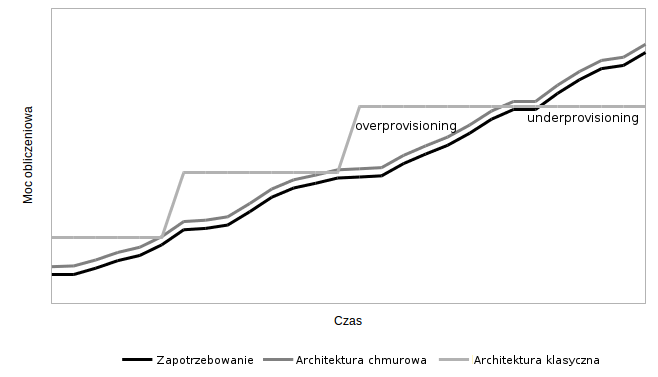
\includegraphics[scale=0.9]{../obrazy/fig:overp.png}
\caption{Tradycyjna architektura wymusza rzadkie zmiany, które skutkują częstym nadmiarem zasobów obliczeniowych. Może on być nawet pogłębiony przez nieoczekiwany spadek zapotrzebowania tuż po zakupieniu dodatkowej mocy obliczeniowej, co generuje dodatkowe koszty. \label{fig:overp}}
\source{Opracowanie własne na podstawie blog.maartenballiauw.be (dostęp 19 czerwca 2017).}
\end{figure}

Korzystając z gotowych rozwiązań oferowanych przez dostawców usług \textit{cloud computingowych} klienci mogą również liczyć na zdecydowanie wyższy poziom bezpieczeństwa niż dotychczas, ponieważ ich dane chronione są przez jedno, wysoce wyspecjalizowane w tym zakresie przedsiębiorstwo.

Tego rodzaju model jest także bardzo opłacalny dla dostawców, ponieważ sposób zarządzania tego rodzaju homogenicznym systemem może być optymalizowany. Według \citet{baun2011} konstruowanie wielkoskalowych rozwiązań chmurowych w tanich lokalizacjach pozwala na obniżenie kosztów elektryczności, połączenia sieciowego, operacji, oprogramowania i sprzętu nawet siedmiokrotnie.

Pojawienie się przetwarzania w chmurze miało stymulujący wpływ na gospodarkę, ale także stawia przed sobą wiele nowych wyzwań. W związku z tym, regulatorzy mają również istotną rolę do odegrania w wielu obszarach:
\begin{itemize}
\item bodźce do używania technologii chmurowych -- rządy muszą odegrać rolę w zachęcaniu wykorzystania \textit{cloud computingu} na przykład poprzez usuwanie zbędnych barier prawnych i regylacyjnych, ale również przez bycie wiodącym ich użytkownikiem i zachęcanie do partnerstw publiczno-prywatnych,
\item standardy -- jednym z wielu wyzwań stojących przed rozwojem chmury jest brak odpowiednich standardów w niektórych obszarach, jak również niedostateczne przyjęcie istniejących standardów. Rządy powinny zachęcać i wspierać rozwój otwartych standardów dla wsparcia biznesu, także poprzez współpracę z różnym instytutami normalizacyjnymi,
\item pomiary -- ilość dostępnych publicznie danych o tego typu przedsięwzięciach jest wciąż niewielka. Regulatorzy, w konsultacji z udziałowcami, powinni odegrać istotną rolę w identyfikowaniu stosownych kryteriów pomiaru wyników i oceny stanu tej gałęzi rynku.
\item kraje rozwijające się -- \textit{cloud computing} daje szansę korzystania ze swoich korzyści przy niskich kosztach dla organizacji i konsumentów pochodzących z krajów rozwijających się. Należy zapewnić odpowiednią infrastrukturę sieciową oraz zachęcać do adaptacji i wykorzystania nowych technologii w owych krajach tak, by mogły one doświadczyć wzrostu ekonomicznego, poprawić zdolności edukacyjne, ale również by umożliwić wolny przepływ informacji dla rozwoju społeczeństwa,
\item konkurencja i handel -- ustawodawcy muszą zadbać o to, by nie dopuścić do niekonkurencyjnych praktyk wynikających z dominacji rynkowej kilku niewielkich przedsiębiorstw. Jest to niezwykle istotne, ponieważ (przywołując również teorię \textit{cloud computingu} jako medium) gałęzie rynku, gdzie kluczowym czynnikiem jest ekonomia skali są szczególnie narażone na tego typu sytuację,
\item podatki -- wraz z migracją wielu centrów danych do chmury, należy rozważyć potencjalny wpływ na rozliczenia podatkowe związane z dostarczaniem tych usług. Szczególnie ważna jest to w przypadku przedsiębiorstw, które dotychczas miały niewielkie doświadczenie w transgranicznych transakcjach i rachunkowości,
\item bezpieczeństwo i zarządzanie ryzykiem -- należy wprowadzić regulacje, które pozwolą trafnie zdefiniować stojące przed \textit{cloud computingiem} wyzwania związane z bezpieczeństwem infrastruktury, w szczególności konieczne jest przeprowadzenie oceny ryzyka, zarządzanie bezpieczeństwem i w efekcie jego usprawnienie,
\item prywatność -- regulatorzy powinni zaadresować pojawiające się pytania dotyczące prywatności przechowywanych danych, takich jak: ,,prawa którego państwa stosuje się do danych przechowywanych w chmurze?'', ,,kto ma dostęp do przechowywanych danych?'', ,,w jakich sytuacjach dane mogą zostać udostępnione jednostkom rządowym?''.
\end{itemize}

\subsubsection{Wiodący dostawcy usług \textit{cloud computingowych}}

\noindent
Według najnowszego raportu ,,Magic Quadrant'' firmy Gartner \citep{leong2017}, liderem rynku pozostaje, niezmiennie od 2006 roku, Amazon Web Services, na kolejnych pozycjach plasują się Microsoft, IBM oraz Google (wyniki rankingu przedstawione zostały na Rysunku \ref{fig:mquad}.). Według \citet{forbes2017}, Amazon posiada 31\% udziału w rynku, Microsoft 11\%, podczas gdy IBM i Google odpowiednio 7\% i 5\%. Jednak, pomimo statusu lidera, Amazon musi czynić intensywne wysiłki by zachować swoją pozycję, ponieważ inni wielcy gracze rozwijają się w imponującym tempie, zdobywając coraz większy udział w rynku infrastruktury chmurowej. Microsoft w czwartym kwartale 2015 powiększył swoje obroty o 124\%, podczas gdy w drugim kwartale 2016 roku to Google odnotował największe tempo wzrostu (162\%). Należy jednocześnie zwrócić uwagę na fakt, że czterech największych graczy stopniowo zwiększa swój udział w rynku (z 51\% w czwartym kwartale 2015 do 54\% w drugim kwartale 2016), por. \citet{forbes2017}.

\begin{figure}[h]
  \centering
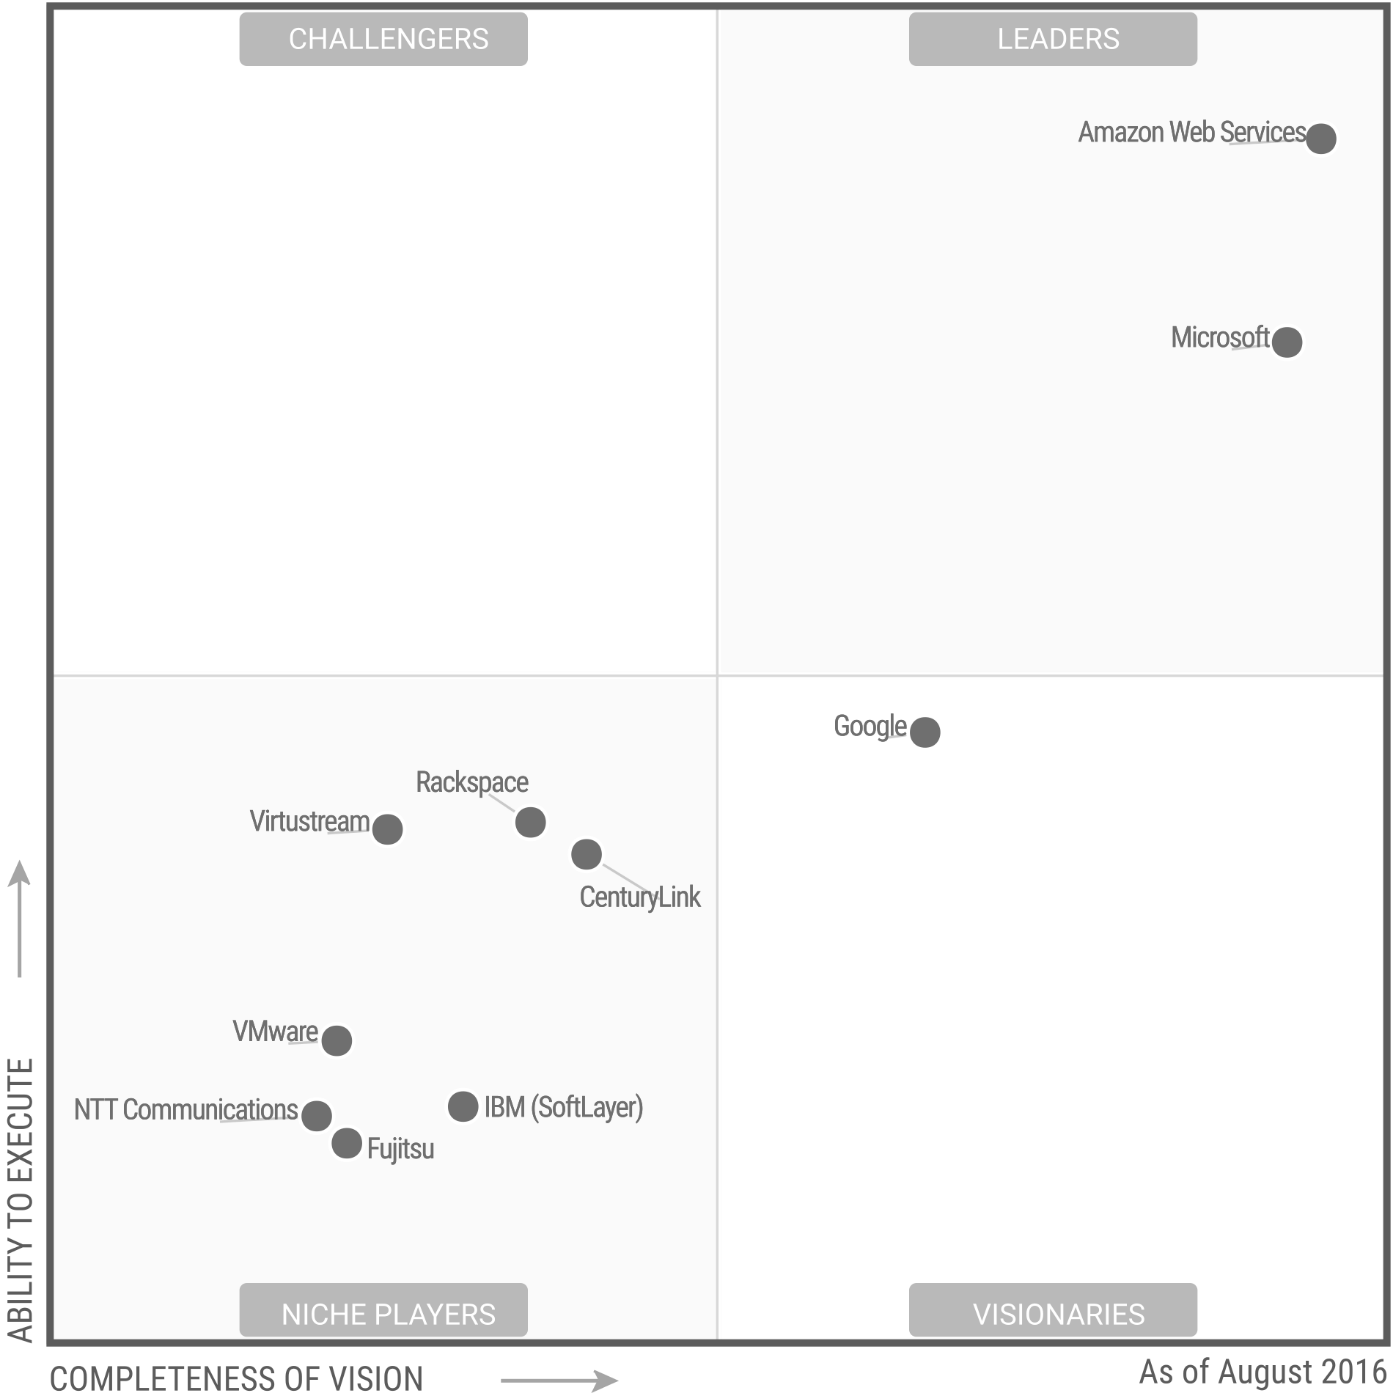
\includegraphics[scale=0.6]{../obrazy/fig:mquad.png}
\caption{\textit{Magic Quadrant} dla przedsiębiorstw oferujących usługi \textit{cloud computingowe} potwierdza status lidera AWS. Należy jednak rozpatrywać Microsoft oraz Google jako równorzędnych konkuretnów.\label{fig:mquad}}
\source{Opracowanie własne na podstawie Gartner (Magic Quadrant for Cloud Infrastructure as a Service, Worldwide)}
\end{figure}

Amazon, pierwszy dostawca usług przetwarzania w chmurze, przechodził stopniową transformację od portalu oferującego książki do online'owego potentata, wykorzystując jednocześnie wysoce innowacyjne rozwiązania do osiągnięcia tego celu. Ta otwartość na innowacje była niejako wymuszona stopniem skomplikowania oferowanego serwisu. Wyświetlenie jednej strony zawierającej informacje o przedmiocie, rekomendacje oraz oceny wymagało licznych, skomplikowanych aplikacji. Ponadto, detaliczny charakter sprzedaży wymagał ciągłego monitorowania zapotrzebowania na zasoby obliczeniowe, ale również obserwowania popytu i wsparcia  procesów operacyjnych systemami informatycznymi (zarówno swoich, jak i partnerów biznesowych). Amazon wykorzystywał technologię wirtualizacji podobnie, jak wiele innych przedsiębiorstw obecnie, by automatycznie i dynamicznie przydzielać zasoby do aplikacji, które tego potrzebowały w danej chwili. Wysoki stopień automatyzacji, który osiągneli w tym zakresie pozwolił im na uruchomienie ich dwóch największych serwisów -  Amazon EC2 (Elastic Compute Cloud) oraz Amazon S3 (Simple Storage System). Amazon EC2 pozwala użytkownikom chmury uruchamiać serwery i zarządzać nimi w jednym z wielu umiejscowionych na różnych kontynentach centrów danych, podczas gdy Amazon S3 jest usługą służącą do przechowywania danych w chmurze. Usługi te miały początkowo zostać udostępnione wewnętrznie i dla partnerów biznesowych, jednak w ramach eksperymentu otwarto je również dla całego świata, gdzie spotkały się z ogromną popularnością, por. \citet{shroff2010}. Ostatecznie doprowadziło do decyzji o uruchomieniu biznesu \textit{cloud computingowego} w 2006 roku. Od tego czasu AWS znacznie rozszerzyło gamę oferowanych usług i dostarcza swoje usługi z wykorzystaniem centrów danych znajdujących się w Ameryce Północnej, Europie, Azji oraz Ameryce Południowej. Do ich silnych stron zaliczana jest duża liczba klientów, najszerszy wachlarz oferowanych usług oraz największe możliwości obliczeniowe, co doprowadziło do ich partnerstwa technologicznego z licznymi przedsiębiorstwami, które dostosowały swoje produkty do uruchamiania na platformie AWS. Z drugiej strony, wymaga to od początkującego użytkownika dużego nakładu czasu, by zaznajomić się z modelem działania i oferowanymi usługami tak, by mógł dostosować je do swoich potrzeb technologicznych.

Microsoft także coraz bardziej skupia się na dostarczaniu swoich możliwości technologicznych z wykorzystaniem usług chmurowych. Platforma przez nich Azure, pozwala na wynajęcie maszyn wirtualnych (z wykorzystaniem oprogramowania Hyper-V), przechowywanie obiektów w chmurze, jak również wiele innych możliwości IaaS oraz PaaS. Ponadto, Azure Marketplace oferuje oprogramowanie i usługi dostarczane przez inne podmioty. Co więcej, Microsoft błyskawicznie wprowadza nowe usługi i funkcjonalności, nakreślając wizję połączonych modeli IaaS oraz PaaS, które współdziałać będą z istniejącą infrastrukturą \textit{on-premises}.  Centra danych Microsoft (określane mianem ,,regionów'') znajdują się nie tylko w Ameryce Północnej i Południowej, Europie i Azji, ale także w Australii. Wartym odnotowania jest również fakt otwarcia się na technologie open source - gama tego typu rozwiązań wspieranych przez Azure wciąż się poszerza, ze szczególnym uwzględnieniem systemów operacyjnych Linux. Microsoft na pewno będzie również korzystał z istniejących kontaktów biznesowych oraz silnej marki, by promować swój produkt i osiągnąć jeszcze większy udział w rynku technologii chmurowych. Choć Azure daleko do stopnia rozwoju i dojrzałości prezentowanego przez AWS, wiele organizacji określa go jako wystarczająco rozbudowany, by móc w niego inwestować.

IBM, jeden z najstarszych koncernów informatycznych, również oferuje usługi \textit{cloud computingowe}. W celu przyspieszenia ekspansji na rynku, w 2013 roku IBM kupiło SoftLayer, niezależnego dostawcę usług chmurowych, by w efekcie ukształtować IBM Cloud Services Division. Przez kolejne lata następowała stopniowa migracja klientów z IBM SmartCloud Enterprise do SoftLayer. Obecnie oferują zarówno wirtualizowane serwery, jak i klasyczne dedykowane maszyny. Ponadto, istnieje także możliwość przechowywania obiektów poprzez zintegrowany CDN (\textit{Content Delivery Network}. Softlayer oferuje swoje usługi z wykorzystaniem centrów danych znajdujących się w Ameryce Północnej, Europie oraz Azji. Do zalet IBM Softlayer, podobnie jak w przypadku, Microsoft, można zaliczyć silną markę oraz liczne kontakty z klientami na całym świecie, co z pewnością pozwoli na rozwój w segmencie przedsiębiorstw. Należy jednak zaznaczyć, że historycznie Softlayer był głównie skupiony na klasycznym modelu dostarczania mocy obliczeniowej i nie rozróżnia na swoim portalu serwisów chmurowych i niechmurowych, brak jest także wielu możliwości technologicznych charakterystycznych dla przetwarzania w chmurze, oferowanych przez liderów rynku.

Google operuje na rynku PaaS pod 2008 roku (oferując swój App Engine), jednakże w modelu IaaS aktywni są dopiero od udostępnienia światu Google Compute Engine w 2013 roku. Obecnie w swojej ofercie łączą zarówno wymienione usługi, jak również wachlarz dodatkowych możliwości, takich jak możliwość przechowywania danych i Container Engine - usługę pozwalającą na konteneryzację, to znaczy uruchomienie aplikacji w wydzielonym konetenerze, ale bez konieczności emulowania warstwy sprzętowej i systemu operacyjnego. Centra danych Google znajdują się w Ameryce Północnej, Europie i Azji. Przez wiele lat prowadzenia własnego biznesu internetowego, Google nabyło szeroką ekspertyzę w projektowaniu tego typu rozwiązań. Niewątpliwą zaletą używania ich serwisu jest możliwość korzystania z ich osiągnięć technologicznych w zakresie wirtualizacji, wykorzystania kontenerów czy też narzędzi do zarządzania klastrami jak Kubernetes. Należy wszakże zaznaczyć, że zakres usług przez nich oferowany nie jest jeszcze tak szeroki jak w przypadku liderów rynku. Według \citet{leong2017}, pomimo szybkiego tempa wzrostu, Google wciąż nie rozwija się dostatecznie dynamicznie, by móc osiągnąć status lidera w tej gałęzi rynku informatycznego.

\clearpage

\section{Eksperymentalne pomiary efektywności kosztowej deep learning}

\noindent
Sukces głębokich sieci neuronowych przypisywany jest ich umiejętności reprezentacji danych wejściowych i odkrywania panujących w nich zależności z wykorzystaniem wielu ukrytych warstw \citep{lecun2015}. Kluczową rolę w ich budowaniu odegrało użycie procesorów graficznych, które pozwoliły na przyspieszenie uczenia tego typu architektur. Ich szerokie wykorzystanie spotkało się z reakcją ze strony dostawców usług \textit{cloud computingowych}, którzy wprowadzili do swoich ofert jednostki wyposażone w procesory graficzne i optymalizowane pod kątem obliczeń naukowych, wynajmując je po wyższych cenach wraz z obietnicą przyspieszenia operacji algebraicznych. Konfiguracje oferowane przez najpopularniejszych dostawców usług przetwarzania w chmurze przedstawione zostały w tabeli \ref{tab:gpu_units}. Spośród największych graczy, Amazon Web Services oraz Microsoft Azure oferują kompletne zestawy, optymalizowane pod kątem obliczeń naukowych (odpowiednio typy p2.* oraz N*), podczas gdy Google Cloud Platform w obecnie obowiązującej wersji beta pozwala na dołączanie kart graficznych do jednej z oferowanych maszyn. Ponadto, można zauważyć, że o ile jednostki podstawowe są bardzo podobne w przypadku AWS i Azure (p2.xlarge oraz NC6), o tyle wzrost dostępnej mocy obliczeniowej bardziej skomplikowanych jednostek jest znacznie szybszy w przypadku AWS. Wyłącznie w ramach Microsoft Azure są również oferowane jednostki nowszej generacji - NVIDIA Tesla M60.

Ponadto, obecnie do wyboru jest także szeroki wachlarz oprogramowania służacego do konstruowania sieci neuronowych, również z wykorzystaniem GPU. Zaliczają się do nich takie narzędzia jak Caffe (Uniwersytet w Berkeley, \citet{jia2014}), CNTK (Microsoft, \citet{yu2014}), MXNet (Distributed Machine Learning Community, \citet{chen2015}), Tensorflow (Google, \citet{abadi2016}), Torch \citep{collobert2011}, Theano (Uniwersytet w Montrealu, \citet{alrhou2016}) oraz Keras (ONEIROS, \citet{chollet2015}). Jednym z głównych zadań problemu uczenia głebokich sieci neuronowych jest znalezienie optymalnego zestawu wag w każdej z warstw sieci, co jest zadaniem, które może zostać sparalelizowane. Każde z wymienionych narzędzi wspiera przetwarzanie równoległe, zarówno z użyciem wielordzeniowych jednostek centralnych, jak i procesorów graficznych. Obliczenia na GPU wykonywane są z pomocą bibliotek dostarczonych przez NVIDIA - cuDNN \citep{chetlur2014}.
Ponadto, obecnie do wyboru jest także szeroki wachlarz oprogramowania służacego do konstruowania sieci neuronowych, również z wykorzystaniem GPU. Zaliczają się do nich takie narzędzia jak Caffe (Uniwersytet w Berkeley, \citet{jia2014}), CNTK (Microsoft Research, \citet{yu2014}), MXNet (Distributed Machine Learning Community, \citet{chen2015}), Tensorflow (Google, \citet{abadi2016}), Torch \citep{collobert2011}, Theano (Uniwersytet w Montrealu, \citet{alrfou2016}) oraz Keras (ONEIROS, \citet{chollet2015}). Jednym z głównych zadań problemu uczenia głebokich sieci neuronowych jest znalezienie optymalnego zestawu wag w każdej z warstw sieci, co jest zadaniem, które może zostać sparalelizowane. Każde z wymienionych narzędzi wspiera przetwarzanie równoległe, zarówno z użyciem wielordzeniowych jednostek centralnych, jak i procesorów graficznych.
Obliczenia na GPU wykonywane są z pomocą bibliotek dostarczonych przez NVIDIA - CUDA oraz cuDNN \citep{chetlur2014}.
W pracy \citet{shi2016} dokonano porównania większości prezentowanych systemów oprogramowania ze sobą i przedstawiono ich silne i słabe strony w popularnych problemach \textit{deep learningowych}.
\noindent
\begin{table}
  \begin{tabular}
    {p{0.08\linewidth}
    p{0.15\linewidth}
    p{0.24\linewidth}
    R{0.08\linewidth}
    R{0.10\linewidth}
    p{0.19\linewidth}}
  \toprule
   & \multicolumn{1}{c}{Typ jednostki} & \multicolumn{1}{c}{Procesor} & \multicolumn{1}{c}{Rdzeni CPU} & \multicolumn{1}{c}{RAM} & \multicolumn{1}{c}{GPU} \\
  \midrule
  AWS & p2.xlarge & Intel Xeon E5-2686v4 & 4 & 61 GB & NVIDIA K80 \\
      & p2.8xlarge & Intel Xeon E5-2686v4 & 32 & 488 GB & 8x NVIDIA K80 \\
      & p2.16xlarge & Intel Xeon E5-2686v4 & 64 & 732 GB & 16x NVIDIA K80 \\
  \midrule
  Azure & NC6 & Intel Xeon E5-2690v3 & 6 & 56 GB & NVIDIA K80 \\
        & NC12 & Intel Xeon E5-2690v3 & 12 & 112 GB & 2x NVIDIA K80 \\
        & NC24(r) & Intel Xeon E5-2690v3 & 24 & 224 GB & 4x NVIDIA K80 \\
        & NV6 & Intel Xeon E5-2690v3 & 6 & 56 GB & NVIDIA M60 \\
        & NV12 & Intel Xeon E5-2690v3 & 12 & 112 GB & 2x NVIDIA M60 \\
        & NV24(r) & Intel Xeon E5-2690v3 & 24 & 224 GB & 4x NVIDIA M60 \\
  \midrule
  GCP & N/D & N/D & N/D & N/D & NVIDIA K80 \\
  \bottomrule
  \end{tabular}
  \caption{Jednostki oferowane przez dostawców usług cloud computingowych. Google Cloud Platform oferuje, w przeciwieństwie do pozostałych dostawców, dokupienie jednostki graficznej do wynajmowanego serwera.}\label{tab:gpu_units}
\end{table}

Istnieje uzasadniona potrzeba pomiaru, na jak dużą oszczędność czasową może liczyć osoba decydująca się na wspomaganie obliczeń naukowych procesorami graficznymi oferowanymi przez platformy \textit{cloud computingowe} i czy wiąże się to z dodatkowymi kosztami. Ekperyment ma na celu empiryczny pomiar czasu potrzebnego na proces generacji różnych architektur głębokich sieci neuronowych, na różnych zbiorach danych i związanego z tym kosztu, wybranie zbioru decyzji niezdominowanych (optymalnych w sensie Pareto), a także dostarczenie narzędzia pozwalającego na przeprowadzanie własnych eksperymentów w tym zakresie.
Spośród przedstawionych w tabeli~\ref{tab:gpu_units} konfiguracji wybrano jednostkę p2.xlarge oferowaną przez Amazon Web Services do porównania z podobnymi jednostkami bez procesorów graficznych ze względu na status lidera rynku i dojrzałość rozwiązań oferowanych przez tego dostawcę. Została porównana z typem instancji, który jest optymalizowany pod kątem obliczeń, z wysokiej jakości jednostką centralną i najniższym stosunkiem ceny do wydajności - c4.2xlarge. Ich specyfikacje techniczne zostały przedstawione w tabeli \ref{tab:aws_units}.
W eksperymencie wykorzystana została także biblioteka Keras, w oparciu o backend Tensorflow. Powodem tej decyzji jest fakt, że została zbudowana w celu ułatwienia przeprowadzania tego typu eksperymentów i oferuje wysoki poziom abstrakcji przy konfigurowaniu architektur bez względu na wykorzystaną u jej podstaw bibliotekę naukową (obecnie możliwe jest wykorzystanie Tensorflow, Theano oraz Deeplearning4j). Należy jednak zaznaczyć, że wszystkie wymienione narzędzia oferują elastyczne API i możliwość edytowania plików konfiguracyjnych dla optymalizowania ich wydajności. Celem przeprowadzanego eksperymentu nie jest porówywanie ich między sobą, nie ustalono zatem jednoznacznie wyższości jednej z bibliotek nad pozostałymi i może istnieć taka konfiguracja, która pozwoli na dalszą optymalizację metody rozwiązania problemu konstruowania sieci neuronowej. Wersje wykorzystanego oprogramowania zostały przedstawione w tabeli~\ref{tab:software}.
\noindent
\begin{table}
  \begin{tabular}
    {p{0.16\linewidth}
    p{0.26\linewidth}
    R{0.09\linewidth}
    R{0.12\linewidth}
    p{0.24\linewidth}}
  \toprule
  \multicolumn{1}{c}{Typ jednostki} & \multicolumn{1}{c}{Procesor} & \multicolumn{1}{c}{Rdzeni CPU} & \multicolumn{1}{c}{RAM} & \multicolumn{1}{c}{GPU} \\
  \midrule
  p2.xlarge & Intel Xeon E5-2686v4 & 4 & 61 GB & NVIDIA K80 \\
  c4.2xlarge & Intel Xeon E5-2666v3 & 8 & 15 GB & brak \\
  \bottomrule
  \end{tabular}
  \caption{Porównywane rodzaje instancji}\label{tab:aws_units}
\end{table}
\noindent
\begin{table}
  \centering
  \begin{tabular}
    {p{0.2\linewidth}
    p{0.4\linewidth}
    R{0.1\linewidth}}
  \toprule
  \multicolumn{1}{c}{Oprogramowanie} & \multicolumn{1}{c}{Twórca} & \multicolumn{1}{c}{Wersja} \\
  \midrule
  Python & Python Software Foundation & 3.5 \\
  Keras & Francois Chollet i inni & 2.0.4 \\
  Tensorflow & Google Brain & 1.1.0 \\
  CUDA & NVIDIA & 7.5 \\
  cuDNN & NVIDIA & 5.1 \\
  \bottomrule
  \end{tabular}
  \caption{W eksperymencie wykorzystano bibliotekę Keras w wersji 2.0.4 opartą o Tensorflow (wersja 1.1.0)}\label{tab:software}
\end{table}

Eksperyment przeprowadzony został z użyciem zbiorów danych będących częstym wyborem w zadaniach porównywania siły predykcyjnej modeli, wydajności sprzętu i oprogramowania - MNIST, IMDB (Large Movie Review Dataset) oraz CIFAR-10. MNIST \citep{lecun1998} jest zbiorem $70~000$ czarno-białych obrazów o rozmiarze 28x28 pikseli, przedstawiających ręcznie pisane cyfry. Pochodzi z większego zbioru danych udostępnionego przez amerykański National Institue of Standards and Technology. Jest częstym wyborem do \textit{benchmarkingu} ze względu na to, że pozwala uniknąć poświęcania znacznej ilości czasu na wstępne przetwarzanie, będąc jednocześnie zbiorem niesyntetycznych danych. Przykładowe obrazy z tego zbioru zaprezentowane zostały na rysunku \ref{fig:mnist_data}.
\begin{figure}[h]
  \centering

\includegraphics[scale=0.5]{../obrazy/fig:mnist_data.png}
\caption{W zbiorze danych MNIST znajdują się obrazy ręcznie pisanych cyfr pochodzących z połączenia dwóch zbiorów danych NIST: Special Database 1 oraz Special Database 3. Special Database 1 zawiera cyfry pisane przez uczniów szkół średnich, podczas gdy Special Database 3 przez United States Census Bureau.\label{fig:mnist_data}}
\source{Opracowanie własne na podstawie \citet{lecun1998}.}
\end{figure}

Large Movie Review Dataset został udostępniony publicznie przez \citet{maas2011}, przy okazji ewaluacji modelu służącego do przeprowadzania analizy sentymentu. Zawiera on przyporządkowanie $50~000$ anonimowych, nieformalnych recenzji filmów na popularnej stronie IMDB do jednej z dwóch rozłącznych grup - pozytywnych i negatywnych.
Przykładowe obserwacje przedstawione zostały w tabeli \ref{tab:imdb_data}. Wstępne przetwarzanie obserwacji sprowadza się do przyjęcia reprezentacji zdania jako wektora indeksów słów, przy czym indeks równy 1 otrzymuje słowo najczęściej występujące w zbiorze danych, 2 -- drugie najczęściej występujące i tak dalej. Pozwala to w łatwy sposób pomijać słowa występujące bardzo rzadko, ale także wyrazy częste, których pojawienie się nie niesie za sobą wystarczającej informacji.
\noindent
\begin{table}
  \begin{tabular}
    {C{0.55\linewidth}
    C{0.35\linewidth}}
  \toprule
  \multicolumn{1}{c}{Nieprzetworzona opinia} & \multicolumn{1}{c}{Klasyfikacja} \\
  \midrule
   If you look at Corey Large's information here on IMDb, apparently there's a movie called ,,Reload'' in production[\ldots] & (-) \\
   Very good drama although it appeared to have a few blank areas [\ldots] & (+) \\
   Weak plot, predictable violence, only semi interesting characters. [\ldots] & (-) \\
  \bottomrule
  \end{tabular}
  \caption{Nieprzetworzone obserwacje pochodzące ze zbioru Large Movie Review Dataset wraz z oceną ich sentymentu - pozytywną (+) lub negatywną (-).\label{tab:imdb_data}}
\end{table}

Trzeci z wykorzystanych zbiorów danych, CIFAR-10 składa się z $60~000$ kolorowych obrazów o rozmiarze 32x32 piksele, równomiernie przyporządkowanych do 10 rozłącznych klas. Jego szczegółowy opis, jak również metodologia zbierania danych została zawarta w pracy \citet{krizhevsky2009}. Wybrane obrazy wchodzące w skład tego zbioru danych przedstawiono na rysunku \ref{fig:cifar_data}.
\begin{figure}[h]
  \centering
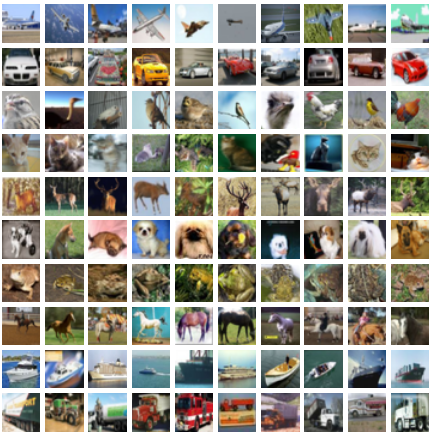
\includegraphics[scale=0.9]{../obrazy/fig:cifar_data.png}
\caption{Każdy z obrazów wchodzących w skład zbioru danych CIFAR-10 został przyporządkowany do jednej z $10$ kategorii (zostały one przedstawione w kolejnych wierszach: airplane, automobile, bird, cat, deer, dog, frog, horse, ship, truck).\label{fig:cifar_data}}
\source{Opracowanie własne na podstawie \citet{krizhevsky2009}.}
\end{figure}

Dla każdego z wybranych zbiorów danych pomiar przeprowadzany jest dla dwóch różnych modeli sieci neuronowych. Zdecydowano się na przeprowadzanie pomiaru z wykorzystaniem sieci konwolucyjnych ze względu na ich szerokie zastosowanie w rozpoznawaniu ukrytych cech danych wejściowych, jak i zadaniach klasyfikacji. W przypadku zbioru danych MNIST wykorzystano architekturę dostępną w ramach biblioteki Keras, jak również stworzoną na jej bazie, bardziej skomplikowaną, sieć konwolucyjną (rysunek \ref{fig:mnist_cnn}). Obie z nich, oprócz jednostek konwolucyjnych, wykorzystują \textit{rectifier} jako funkcję aktywacji w warstwach ukrytych i \textit{softmax} w warstwie wyjściowej, \textit{max pooling}, \textit{dropout} oraz \textit{fully connected layers}. Jako funkcję straty zdefiniowano \textit{cross entropy}. Domyślny model wykorzystuje ponadto ADADELTA jako metodę optymalizacyjną opartą na spadku gradientowym. Metoda ta okazała się skuteczniejsza od klasycznego algorytmu \textit{stochastic gradient descent}
na zbiorze danych MNIST \citep{zeiler2012}. Niestandardowy model korzysta z RMSprop jako algorytmu optymalizacyjnego, por. \citet{tieleman2012}. Uczenie w przypadku domyślnego modelu odbywa się poprzez wykonanie $10$ iteracji przez zbiór danych (\textit{epoch}), gdzie jedna partia (\textit{mini-batch}) składa się ze $128$ obserwacji. Te wartości wynoszą odpowiednio $36$ i $64$ w przypadku drugiego modelu.
\begin{figure}[h]
  \centering
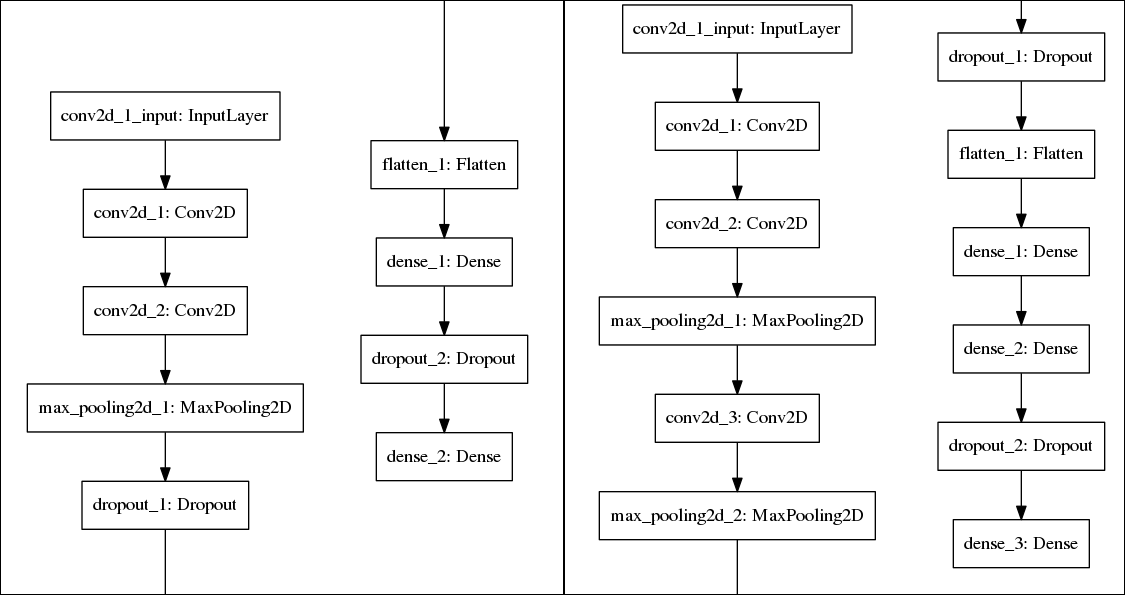
\includegraphics[scale=0.35]{../obrazy/fig:mnist_cnn.png}
\caption{Modele sieci konwolucyjnych zbudowane dla zbioru MNIST. Architektura dostępna w ramach biblioteki Keras zaprezentowana została po lewej stronie, po prawej architektura niestandardowa.\label{fig:mnist_cnn}}
\source{Opracowanie własne.}
\end{figure}

Dla zbioru IMDB wykorzystano dwie architektury dostępne w ramach biblioteki Keras - jednokierunkową (\textit{feedforward}) oraz rekurencyjną (\textit{recurrent}) sieć konwolucyjną (rysunek \ref{fig:imdb_cnn}). Pierwszy model ogranicza słownik do $5~000$ słów, podczas gdy drugi do $20~000$. Jako maksymalną długość recenzji przyjęto odpowiednio $400$ i $100$ słów (przy czym dla zdań krótszych niż zadana długość wykorzystywany jest \textit{padding}). W obu modelach pierwszą warstwą jest warstwa typu \textit{embedding}, która otrzymuje sekwencje pozytywnych liczb całkowitych (w tym wypadku indeksów wyrazów) i zwraca ich reprezentację macierzową o zadanej długości. Bazuje ona na technikach \textit{word embedding} oraz algorytmach Word2Vec, które przyjmując wyrazy (indeksy wyrazów) znajdujące się w dyskretnej przestrzeni (słowniku), zwracają ich reprezentację w przestrzeni ciągłej (jako wektor liczb rzeczywistych), por. \citep{goldberg2014}. Intuicja stojąca za tymi technikami każe sądzić, że podobne semantycznie słowa znajdą się blisko siebie w tak stworzonej, n-wymiarowej przestrzeni.
W obu sieciach również wykorzystywane są \textit{max pooling}, \textit{dropout} oraz \textit{fully connected layers}. Rekurencyjna architektura wykorzystuje ponadto warstwę jednostek LSTM (\textit{Long-Short Term Memory Units}, por. \citet{hochreiter1997}. Ich wprowadzenie było odpowiedzią na problem znikającego lub eksplodującego gradientu \citep{hochreiter1991}. W modelu LSTM przedstawiono nową strukturę, nazwaną mianem komórki pamięci \textit{memory cell} (rysunek \ref{fig:lstm_memcell}). Składa się z czterech głównych komponentów: bramki wejściowej, neuronu z rekurencyjnym połączeniem, bramki pamięci (\textit{forget cell}) oraz bramki wyjściowej.
Połączenie rekurencyjne ma wagę $1$ i ma na celu zapewnienie, że \textit{ceteris paribus}, stan komórki pozostanie niezmieniony przy przejściu z czasu $t$ do czasu $t+1$. Bramki mają na celu kontrolowanie interakcji neuronu z otoczeniem. Bramka wejściowa może pozwolić na zmianę jego stanu przez sygnał wejściowy lub blokować taką próbę. Z drugiej strony, bramka wyjściowa może zezwalać lub zabraniać dokonywaniu zmian w innych neuronach przez \textit{memory cell}. Wreszcie, \textit{forget cell} kontroluje połączenie rekurencyjne, decydując czy jednostka ,,pamięta'', czy ,,zapomina'' swój poprzedni stan. Architektura tego typu jednostki przedstawiona została na rysunku \ref{fig:lstm_memcell}. Algorytmem optymalizacyjnym w obu modelach jest Adam, metoda oparta na momentach gradientu niskiego rzędu, wymagająca niewielkiej ilości pamięci operacyjnej, por. \citet{kingma2014}.
\begin{figure}[h]
  \centering
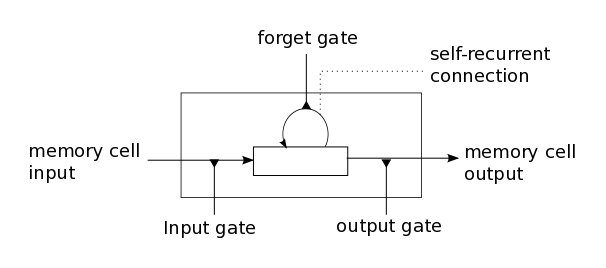
\includegraphics[scale=0.4]{../obrazy/fig:lstm_memcell.png}
\caption{Jednostka \textit{Long-Short Term Memory}. Oprócz klasycznej architektury neuronu z połączeniem rekurencyjnym, elementami wchodzącymi w jej skład są trzy bramki: wejściowa (\textit{input gate}), pamięci (\textit{forget gate}) i wyjściowa (\textit{output gate}).\label{fig:lstm_memcell}}
\source{Opracowanie własne.}
\end{figure}
\begin{figure}[h]
  \centering
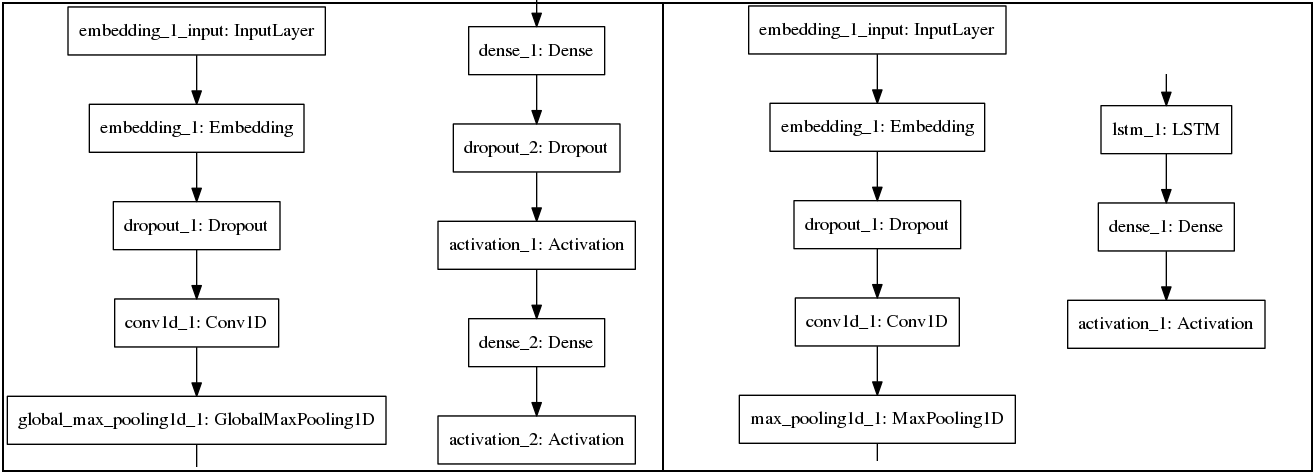
\includegraphics[scale=0.35]{../obrazy/fig:imdb_cnn.png}
\caption{Architektury zbudowane dla zbioru Large Movie Review Dataset. Po lewej stronie przedstawiono model sieci jednokierunkowej, po prawej zilustrowano model sieci rekurencyjnej.\label{fig:imdb_cnn}}
\source{Opracowanie własne.}
\end{figure}

Dla zbioru CIFAR-10 eksperyment również przeprowadzany jest z wykorzystaniem dwóch rodzajów sieci konwolucyjnych. Pierwsza z nich udostępniona została w bibliotece Keras, podczas gdy druga jest jej rozszerzeniem. W obu zastosowano warstwy konwolucyjne, \textit{fully connected layers}, ale także \textit{rectified linear units} i \textit{dropout}. Domyślny model wykorzystuje ponadto warstwy \textit{max poolingowe} i RMSprop jako algorytm optymalizacyjny. \textit{Mini-batch} składa się z $32$ obserwacji, podczasy gdy liczba iteracji przez zbiór danych wynosi $200$. W przypadku niestandardowej architektury wykorzystano technikę \textit{average pooling}, a algorytmem optymalizującym jest ADADELTA. Liczba obserwacji przypadających na jedną partię uczącą wynosi $64$, a liczba iteracji $300$. Architektury tak stworzonych modeli przedstawiono na rysunku \ref{fig:cifar_cnn}.
\begin{figure}[h]
  \centering
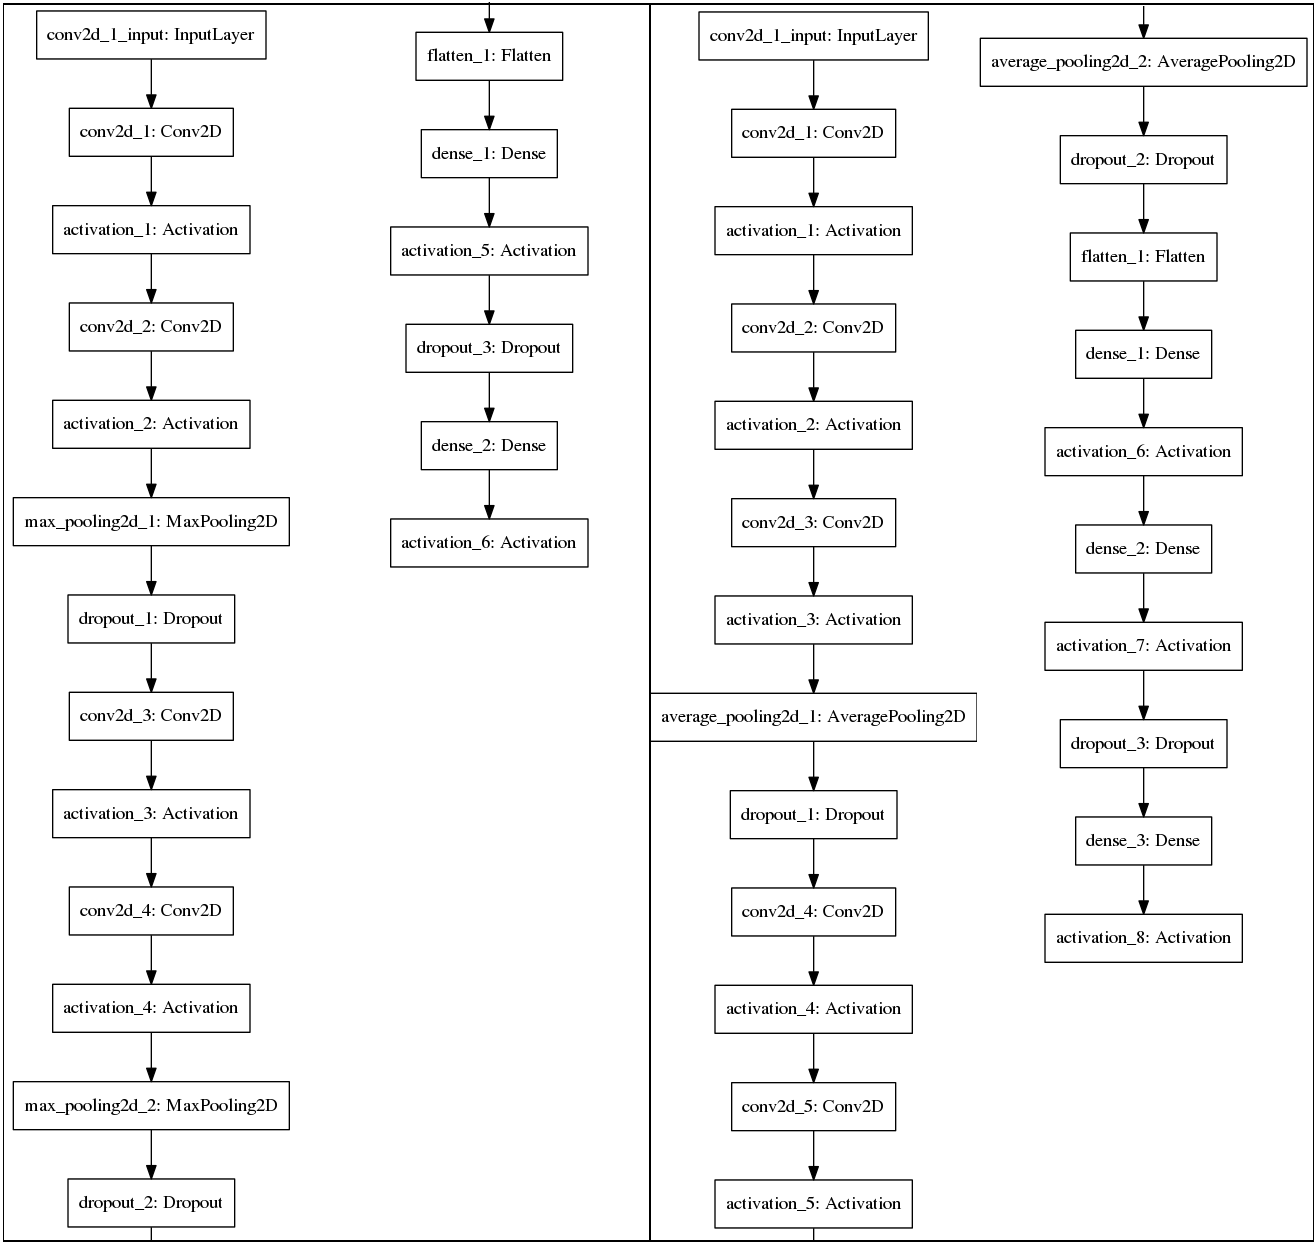
\includegraphics[scale=0.35]{../obrazy/fig:cifar_cnn.png}
\caption{Podobnie jak w przypadku zbioru danych MNIST, na rysunku przedstawiono architekturę domyślną (lewa strona) oraz rozbudowaną (prawa strona).\label{fig:cifar_cnn}}
\source{Opracowanie własne.}
\end{figure}

\clearpage

\section{Efektywność kosztowa głębokich sieci neuronowych w chmurze}

\noindent
Analizowanymi w eksperymencie miarami są czas potrzebny na naukę modelu sieci neuronowej, ilość pracy potrzebna na osiągnięcie tego celu oraz wskaźniki oceny jakości modelu takie jak jego trafność i wartości funkcji straty dla zbioru treningowego i walidacyjnego. Otrzymane rezultaty prezentowane są w podziale na poszczególne zbiory danych, architektury modeli i typy jednostki, na której wykonywane były obliczenia.

Tabela \ref{tab:experiment_results} przedstawia czasy potrzebne na wykonanie jednej iteracji przez zbiór danych (\textit{epoch}) w postaci średnia $\pm$ odchylenie standardowe. Wykorzystanie jednostek posiadających procesory graficzne pozwala na przyspieszenie obliczeń pięcio-, a nawet dwunastokrotnie w porównaniu do serwerów nie wyposażonych w \textit{GPU} dla jednokierunkowych sieci konwolucyjnych. W przypadku sieci rekurencyjnej, w której wykorzystane są jednostki typu LSTM, różnica jest zdecydowanie mniejsza (ok. $40$ sekund w porównaniu do ok. $46$ sekund). Pomiary czasów uczenia wykazują bardzo niewielkie wahania (wykresy pudełkowe ilustrujące porównanie dla dwóch rodzajów instancji przedstawione są na rysunku \ref{fig:experiment_results}), z wyjątkiem pierwszej iteracji, która w przypadku rekurencyjnej architektury dla zbioru danych IMDB (\textit{lstmkerasdef} oraz architektury niestandardowej dla zbioru danych MNIST (\textit{kerasdef}) trwała znacznie dłużej niż kolejne.
\noindent
\begin{table}
  \begin{tabular}
    {C{0.21\linewidth}
    C{0.21\linewidth}
    C{0.21\linewidth}
    R{0.26\linewidth}
    }
  \toprule
  \multicolumn{1}{C{0.15\linewidth}}{Zbiór danych} & \multicolumn{1}{C{0.15\linewidth}}{Architektura} & \multicolumn{1}{C{0.15\linewidth}}{Typ instancji} & \multicolumn{1}{C{0.2\linewidth}}{Czas (s)}\\
  \midrule
  cifar & custom & c4.2xlarge &  $133.11\pm0.32$ \\
        &        & p2.xlarge &   $20.15\pm0.12$ \\
        & kerasdef & c4.2xlarge &  $116.36\pm0.45$ \\
        &        & p2.xlarge &    $21.65\pm0.1$ \\
  imdb &        & c4.2xlarge &  $124.71\pm0.12$ \\
        &        & p2.xlarge &   $10.23\pm0.44$ \\
        & lstm kerasdef & c4.2xlarge &   $45.94\pm0.43$ \\
        &        & p2.xlarge &   $39.94\pm1.22$ \\
  mnist & custom & c4.2xlarge &   $94.28\pm0.23$ \\
        &        & p2.xlarge &   $12.81\pm0.21$ \\
        & kerasdef & c4.2xlarge &    $81.5\pm2.68$ \\
        &        & p2.xlarge &  $16.73\pm21.45$ \\
  \bottomrule
  \end{tabular}
  \caption{Czasy potrzebne na wykonanie jednej iteracji przez wszystkie obserwacje podczas uczenia modelu sieci neuronowej dla poszczególnych zbiorów danych i architektur.\label{tab:experiment_results}}
\end{table}
\begin{figure}[h]
  \centering
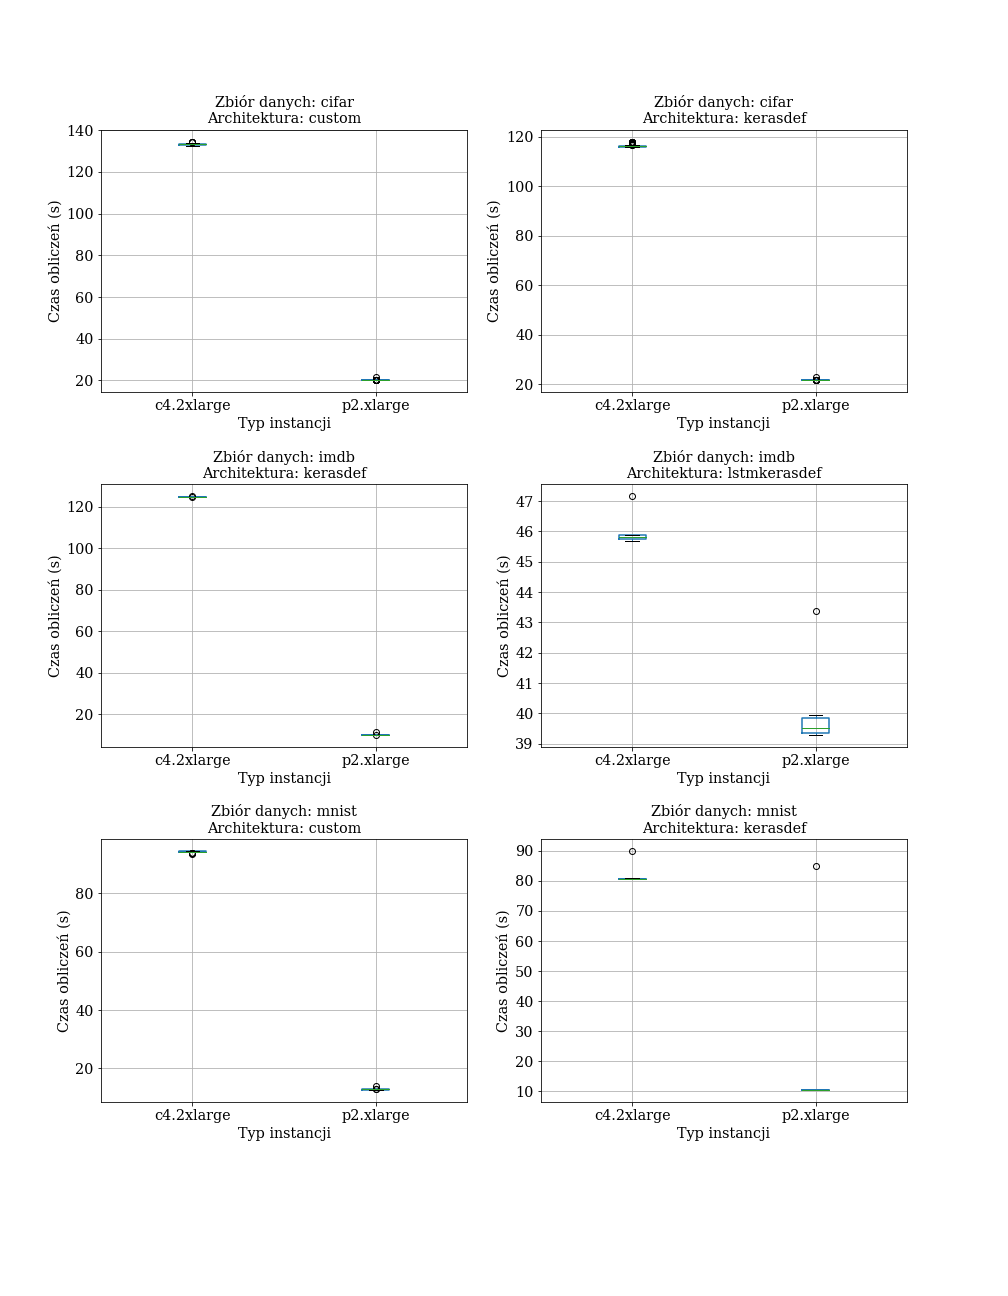
\includegraphics[scale=0.5]{../obrazy/fig:experiment_results.png}
\caption{Wykresy pudełkowe czasów potrzebnych na jedną iterację przez zbiór danych.\label{fig:experiment_results}}
\source{Opracowanie własne.}
\end{figure}

Ceny wykorzystywanych instancji na rynku spot i on-demand zostały zaprezentowane w tabeli \ref{tab:instance_prices}. W przypadku cen on-demand instancje p2.xlarge są o $126\%$ droższe w porównaniu do c4.2xlarge. Jest to stosunek cen, który, biorąc pod uwagę różnicę w czasie potrzebnym na zbudowaniu modelu, sugeruje wybór jednostki wyposażonej w GPU. Pozwoli to na oszczędność czasu potrzebnego na obliczenia, ale także prowadzi do optymalizacji kosztowej.
Stosowanie jednostek wyposażonych w GPU jest również rekomendowane w przypadku decydowana się na wynajem instancji na rynku spot, gdzie średnia (mediana) ceny instancji p2.xlarge w czasie przeprowadzanego eksperymentu była o $124\%$ ($129\%$) wyższa od średniej (mediany) ceny instancji c4.2xlarge.

Nakład pracy potrzebny na skonstruowanie sieci neuronowej z wykorzystaniem maszyny wyposażonej w procesor graficzny jest taki sam, jak w przypadku serwera nie wyposażonego w GPU. Powodem tego stanu rzeczy jest wykorzystanie wysokopoziomowych bibliotek (Keras oraz Tensorflow lub Theano), które automatycznie wykrywają obecność kart graficznych przystosowanych do obliczeń naukowych oraz sterowników pochodzących od NVIDIA (CUDA, cudNN) i dostosowują do tego sposób przydzielania zadań.

Należy zatem pozytywnie zweryfikować postawione hipotezy badawcze -- stosowanie jednostek wykorzystujących GPU, oferowanych w Amazon Web Services, jest rozwiązaniem efektywnym kosztowo w porównaniu do jednostek wyposażonych wyłącznie w CPU. Ponadto, wykorzystywanie przedstawionego narzędzia pozwala na porównanie czasu potrzebnego na uczenie dla wybranych zbiorów danych, architektur i wybór optymalnego dla danego problemu rozwiązania.
\noindent
\begin{table}
  \begin{tabular}
    {C{0.16\linewidth}
    R{0.24\linewidth}
    R{0.24\linewidth}
    R{0.25\linewidth}}
  \toprule
  \multicolumn{1}{C{0.15\linewidth}}{Typ jednostki} & \multicolumn{1}{C{0.22\linewidth}}{Cena on-demand (\$)} & \multicolumn{1}{C{0.22\linewidth}}{Cena spot (średnia, \$)} & \multicolumn{1}{C{0.22\linewidth}}{Cena spot (mediana, \$)} \\
  \midrule
  p2.xlarge & $0.9000$ & $0.2450$ & $0.2489$ \\
  c4.2xlarge & $0.3980$ & $0.1092$ & $0.1085$ \\
  \bottomrule
  \end{tabular}
  \caption{Ceny instancji na rynku on-demand oraz spot w czasie przeprowadzania eksperymentu.}\label{tab:instance_prices}
\end{table}

W tabelach
(\ref{tab:experiment_metrics},
\ref{tab:experiment_times_cifar},
\ref{tab:experiment_times_imdb},
\ref{tab:experiment_times_mnist})
oraz na wykresach
(\ref{fig:experiment_loss_timecum}, \ref{fig:experiment_loss_price_ond},
\ref{fig:experiment_loss_val_timecum}, \ref{fig:experiment_loss_val_price_ond},
\ref{fig:experiment_acc_timecum}, \ref{fig:experiment_acc_price_ond},
\ref{fig:experiment_acc_val_timecum}, \ref{fig:experiment_acc_val_price_ond})
przedstawiono metryki jakości estymowanych modeli - funkcję straty i trafność oraz potrzebny do ich osiągnięcia czas i koszt. Ostatecznie z wykorzystaniem obu typów instancji osiągnięto podobne wyniki, jednakże z wyjątkiem sieci rekurencyjnej wartość funkcji straty czy trafności znacznie szybciej asymptotycznie zbiega do wartości granicznej w przypadku serwerów wyposażonych w procesory graficzne (por. także w tabeli \ref{tab:experiment_results}). Koszt potrzebny na osiągnięcie wyznaczonych poziomów trafności modelu również jest wielokrotnie niższy dla instancji GPU (około pięcio-, a nawet siedmiokrotnie, por. między innymi w tabeli \ref{tab:experiment_times_cifar}) w porównaniu do instancji c4.2xlarge.

Analizując miary służące oceny estymowanych modeli można zauważyć, że o ile modyfikacja domyślnej architektury prowadziła do uzyskania lepszego modelu dla zbioru danych CIFAR-10 (trafność na zbiorze walidacyjnym architektury \textit{custom} wyniosła około $0,87$, a dla architektury \textit{kerasdef} około $0,79$), o tyle dla zbioru MNIST nie poskutkowała znaczną różnicą w wynikach. Ponadto, w przypadku obu architektur stworzonych dla zbioru danych IMDB, jak również w przypadku architektury domyślnej dla zbioru danych CIFAR-10 miało miejsce przeuczenie sieci neuronowej. Nie jest ona w stanie wystarczająco dobrze uogólniać odkryte zależności na obserwacje nie pochodzące ze zbioru treningowego, co skutkuje wzrostem funkcji straty (spadkiem trafności) na zbiorze walidacyjnym. Występuje on po 2. iteracji w przypadku architektur zbudowanych na potrzeby zbioru danych IMDB i po około 120. iteracji modelu domyślnego dla CIFAR-10.
%Wynika to z faktu, że liczba iteracji przez zbiór danych była jednak ustalana na potrzeby pomiaru czasu przypadającego na jeden \textit{epoch}, nie na potrzeby uzyskania najlepszego modelu.
\noindent
\begin{table}
  \begin{tabular}
    {C{0.1\linewidth}
    C{0.12\linewidth}
    C{0.1\linewidth}
    R{0.12\linewidth}
    R{0.12\linewidth}
    R{0.12\linewidth}
    R{0.12\linewidth}
    }
  \toprule
  \multicolumn{1}{C{0.1\linewidth}}{Zbiór danych} & \multicolumn{1}{C{0.12\linewidth}}{Architektura} & \multicolumn{1}{C{0.1\linewidth}}{Typ instancji} & \multicolumn{1}{C{0.12\linewidth}}{Funkcja straty (zbiór trening.)} & \multicolumn{1}{C{0.12\linewidth}}{Funkcja straty (zbiór walid.)} & \multicolumn{1}{C{0.12\linewidth}}{Trafność (zbiór trening.)} & \multicolumn{1}{C{0.12\linewidth}}{Trafność (zbiór walid.)} \\
  \midrule
  cifar & custom & c4.2xlarge &                           $0.2180$ &                           $0.4204$ &                    $0.9309$ &                     $0.8743$ \\
        &        & p2.xlarge &                          $0.2207$ &                           $0.4083$ &                    $0.9308$ &                     $0.8767$ \\
        & kerasdef & c4.2xlarge &                          $0.6217$ &                           $0.6494$ &                    $0.7935$ &                     $0.7874$ \\
        &        & p2.xlarge &                          $0.6031$ &                           $0.6331$ &                    $0.8004$ &                     $0.7967$ \\
  imdb & kerasdef & c4.2xlarge &                           $0.0290$ &                           $0.2706$ &                    $0.9896$ &                     $0.8864$ \\
        &        & p2.xlarge &                          $0.0292$ &                           $0.2838$ &                    $0.9894$ &                     $0.8871$ \\
        & lstm kerasdef & c4.2xlarge &                          $0.0079$ &                           $0.3594$ &                    $0.9972$ &                     $0.8482$ \\
        &        & p2.xlarge &                          $0.0095$ &                           $0.3701$ &                    $0.9969$ &                     $0.8515$ \\
  mnist & custom & c4.2xlarge &                          $0.1184$ &                            $0.0260$ &                    $0.9679$ &                     $0.9921$ \\
        &        & p2.xlarge &                          $0.1183$ &                           $0.0292$ &                    $0.9691$ &                     $0.9913$ \\
        & kerasdef & c4.2xlarge &                          $0.0366$ &                           $0.0265$ &                    $0.9889$ &                     $0.9916$ \\
        &        & p2.xlarge &                          $0.0384$ &                           $0.0275$ &                    $0.9889$ &                     $0.9904$ \\
  \bottomrule
  \end{tabular}
  \caption{Wartości funkcji celu i trafności dla zbioru treningowego i walidacyjnego w konstruowanych architekturach sieci.\label{tab:experiment_metrics}}
\end{table}
\noindent
\begin{table}
  \begin{tabular}
    {C{0.1\linewidth}
    C{0.12\linewidth}
    C{0.1\linewidth}
    C{0.08\linewidth}
    R{0.1\linewidth}
    R{0.1\linewidth}
    R{0.12\linewidth}
    R{0.12\linewidth}
    }
  \toprule
  \multicolumn{1}{C{0.1\linewidth}}{Zbiór danych} & \multicolumn{1}{C{0.12\linewidth}}{Architektura} & \multicolumn{1}{C{0.1\linewidth}}{Typ instancji} & \multicolumn{1}{C{0.08\linewidth}}{Kwant.} & \multicolumn{1}{C{0.1\linewidth}}{Trafność (zbiór trening.)} & \multicolumn{1}{C{0.1\linewidth}}{Czas (s)} & \multicolumn{1}{C{0.12\linewidth}}{Cena on-demand (\$)} & \multicolumn{1}{C{0.12\linewidth}}{Cena spot (średnia, \$)} \\
  \midrule
  cifar & custom & c4.2xlarge & $0.10$ &  $0.8288$ &  $133.44$ &     $0.4573$ &      $0.1255$ \\
        &        &            & $0.25$ &  $0.8923$ &  $133.21$ &     $1.1061$ &      $0.3035$ \\
        &        &            & $0.50$ &  $0.9211$ &  $132.83$ &     $2.4315$ &      $0.6671$ \\
        &        &            & $0.75$ &  $0.9271$ &  $132.85$ &     $3.5771$ &      $0.9815$ \\
        &        &            & $0.90$ &  $0.9284$ &  $132.81$ &     $3.4304$ &      $0.9412$ \\
        &        & p2.xlarge & $0.10$ &  $0.8317$ &   $20.27$ &     $0.1569$ &      $0.0427$ \\
        &        &            & $0.25$ &  $0.8938$ &   $20.06$ &     $0.3837$ &      $0.1045$ \\
        &        &            & $0.50$ &  $0.9218$ &   $20.28$ &     $0.8066$ &      $0.2196$ \\
        &        &            & $0.75$ &  $0.9270$ &   $20.09$ &     $1.3955$ &      $0.3799$ \\
        &        &            & $0.90$ &  $0.9280$ &   $20.09$ &     $1.0029$ &      $0.2730$ \\
        & kerasdef & c4.2xlarge & $0.10$ &  $0.7061$ &  $116.30$ &     $0.1800$ &      $0.0494$ \\
        &        &            & $0.25$ &  $0.7445$ &  $116.07$ &     $0.2956$ &      $0.0811$ \\
        &        &            & $0.50$ &  $0.7781$ &  $116.42$ &     $1.8107$ &      $0.4968$ \\
        &        &            & $0.75$ &  $0.7881$ &  $116.25$ &     $1.5150$ &      $0.4157$ \\
        &        &            & $0.90$ &  $0.7903$ &  $116.01$ &     $1.2323$ &      $0.3381$ \\
        &        & p2.xlarge & $0.10$ &  $0.7290$ &   $21.63$ &     $1.0610$ &      $0.2888$ \\
        &        &            & $0.25$ &  $0.7609$ &   $21.67$ &     $0.9473$ &      $0.2579$ \\
        &        &            & $0.50$ &  $0.7875$ &   $21.64$ &     $0.2817$ &      $0.0767$ \\
        &        &            & $0.75$ &  $0.7951$ &   $21.66$ &     $0.3466$ &      $0.0944$ \\
        &        &            & $0.90$ &  $0.7969$ &   $21.64$ &     $0.3791$ &      $0.1032$ \\
  \bottomrule
  \end{tabular}
  \caption{Czas oraz koszt potrzebny na osiągnięcie ustalonych poziomów trafności na zbiorze treningowym dla zbioru danych CIFAR-10.\label{tab:experiment_times_cifar}}
\end{table}
\begin{table}
  \begin{tabular}
    {C{0.1\linewidth}
    C{0.12\linewidth}
    C{0.1\linewidth}
    C{0.08\linewidth}
    R{0.1\linewidth}
    R{0.1\linewidth}
    R{0.12\linewidth}
    R{0.12\linewidth}
    }
  \toprule
  \multicolumn{1}{C{0.1\linewidth}}{Zbiór danych} & \multicolumn{1}{C{0.12\linewidth}}{Architektura} & \multicolumn{1}{C{0.1\linewidth}}{Typ instancji} & \multicolumn{1}{C{0.08\linewidth}}{Kwant.} & \multicolumn{1}{C{0.1\linewidth}}{Trafność (zbiór trening.)} & \multicolumn{1}{C{0.1\linewidth}}{Czas (s)} & \multicolumn{1}{C{0.12\linewidth}}{Cena on-demand (\$)} & \multicolumn{1}{C{0.12\linewidth}}{Cena spot (średnia, \$)} \\
  \midrule
  imdb &        & c4.2xlarge & $0.10$ &  $0.9000$ &  $124.67$ &     $0.0276$ &      $0.0076$ \\
        &        &            & $0.25$ &  $0.9318$ &  $124.69$ &     $0.0414$ &      $0.0114$ \\
        &        &            & $0.50$ &  $0.9744$ &  $124.74$ &     $0.0690$ &      $0.0189$ \\
        &        &            & $0.75$ &  $0.9842$ &  $124.66$ &     $0.0965$ &      $0.0265$ \\
        &        &            & $0.90$ &  $0.9878$ &  $124.71$ &     $0.1241$ &      $0.0340$ \\
        &        & p2.xlarge & $0.10$ &  $0.9025$ &   $10.09$ &     $0.0054$ &      $0.0015$ \\
        &        &            & $0.25$ &  $0.9341$ &   $10.08$ &     $0.0079$ &      $0.0022$ \\
        &        &            & $0.50$ &  $0.9702$ &   $10.09$ &     $0.0130$ &      $0.0035$ \\
        &        &            & $0.75$ &  $0.9835$ &   $10.09$ &     $0.0205$ &      $0.0056$ \\
        &        &            & $0.90$ &  $0.9876$ &   $10.09$ &     $0.0231$ &      $0.0063$ \\
        & lstmkerasdef & c4.2xlarge & $0.10$ &  $0.9254$ &   $45.83$ &     $0.0103$ &      $0.0028$ \\
        &        &            & $0.25$ &  $0.9671$ &   $45.81$ &     $0.0153$ &      $0.0042$ \\
        &        &            & $0.50$ &  $0.9920$ &   $45.89$ &     $0.0255$ &      $0.0070$ \\
        &        &            & $0.75$ &  $0.9942$ &   $45.77$ &     $0.0356$ &      $0.0098$ \\
        &        &            & $0.90$ &  $0.9957$ &   $45.76$ &     $0.0457$ &      $0.0125$ \\
        &        & p2.xlarge & $0.10$ &  $0.9245$ &   $39.90$ &     $0.0208$ &      $0.0057$ \\
        &        &            & $0.25$ &  $0.9651$ &   $39.59$ &     $0.0307$ &      $0.0084$ \\
        &        &            & $0.50$ &  $0.9908$ &   $39.47$ &     $0.0505$ &      $0.0138$ \\
        &        &            & $0.75$ &  $0.9956$ &   $39.35$ &     $0.0802$ &      $0.0218$ \\
        &        &            & $0.90$ &  $0.9964$ &   $39.45$ &     $0.0900$ &      $0.0245$ \\
  \bottomrule
  \end{tabular}
  \caption{Czas oraz koszt potrzebny na osiągnięcie ustalonych poziomów trafności na zbiorze treningowym dla zbioru danych IMDB.\label{tab:experiment_times_imdb}}
\end{table}
\begin{table}
  \begin{tabular}
    {C{0.1\linewidth}
    C{0.12\linewidth}
    C{0.1\linewidth}
    C{0.08\linewidth}
    R{0.1\linewidth}
    R{0.1\linewidth}
    R{0.12\linewidth}
    R{0.12\linewidth}
    }
  \toprule
  \multicolumn{1}{C{0.1\linewidth}}{Zbiór danych} & \multicolumn{1}{C{0.12\linewidth}}{Architektura} & \multicolumn{1}{C{0.1\linewidth}}{Typ instancji} & \multicolumn{1}{C{0.08\linewidth}}{Kwant.} & \multicolumn{1}{C{0.1\linewidth}}{Trafność (zbiór trening.)} & \multicolumn{1}{C{0.1\linewidth}}{Czas (s)} & \multicolumn{1}{C{0.12\linewidth}}{Cena on-demand (\$)} & \multicolumn{1}{C{0.12\linewidth}}{Cena spot (średnia, \$)} \\
  \midrule
  mnist & custom & c4.2xlarge & $0.10$ &  $0.8716$ &   $93.91$ &     $0.0518$ &      $0.0142$ \\
        &        &            & $0.25$ &  $0.9248$ &   $94.14$ &     $0.1039$ &      $0.0285$ \\
        &        &            & $0.50$ &  $0.9538$ &   $94.55$ &     $0.1979$ &      $0.0543$ \\
        &        &            & $0.75$ &  $0.9627$ &   $94.46$ &     $0.2709$ &      $0.0743$ \\
        &        &            & $0.90$ &  $0.9668$ &   $94.56$ &     $0.3439$ &      $0.0944$ \\
        &        & p2.xlarge & $0.10$ &  $0.8770$ &   $12.76$ &     $0.0163$ &      $0.0044$ \\
        &        &            & $0.25$ &  $0.9269$ &   $12.80$ &     $0.0322$ &      $0.0088$ \\
        &        &            & $0.50$ &  $0.9557$ &   $12.82$ &     $0.0610$ &      $0.0166$ \\
        &        &            & $0.75$ &  $0.9633$ &   $12.84$ &     $0.0865$ &      $0.0236$ \\
        &        &            & $0.90$ &  $0.9674$ &   $12.77$ &     $0.1089$ &      $0.0296$ \\
        & kerasdef & c4.2xlarge & $0.10$ &  $0.9649$ &   $80.74$ &     $0.0189$ &      $0.0052$ \\
        &        &            & $0.25$ &  $0.9780$ &   $80.74$ &     $0.0367$ &      $0.0101$ \\
        &        &            & $0.50$ &  $0.9842$ &   $80.71$ &     $0.0635$ &      $0.0174$ \\
        &        &            & $0.75$ &  $0.9874$ &   $80.72$ &     $0.0813$ &      $0.0223$ \\
        &        &            & $0.90$ &  $0.9882$ &   $80.71$ &     $0.0992$ &      $0.0272$ \\
        &        & p2.xlarge & $0.10$ &  $0.9662$ &   $10.53$ &     $0.0238$ &      $0.0065$ \\
        &        &            & $0.25$ &  $0.9782$ &   $10.54$ &     $0.0291$ &      $0.0079$ \\
        &        &            & $0.50$ &  $0.9843$ &   $10.53$ &     $0.0370$ &      $0.0101$ \\
        &        &            & $0.75$ &  $0.9872$ &   $10.53$ &     $0.0423$ &      $0.0115$ \\
        &        &            & $0.90$ &  $0.9881$ &   $10.54$ &     $0.0475$ &      $0.0129$ \\
  \bottomrule
  \end{tabular}
  \caption{Czas oraz koszt potrzebny na osiągnięcie ustalonych poziomów trafności na zbiorze treningowym dla zbioru danych MNIST.\label{tab:experiment_times_mnist}}
\end{table}
\begin{figure}[h]
  \centering
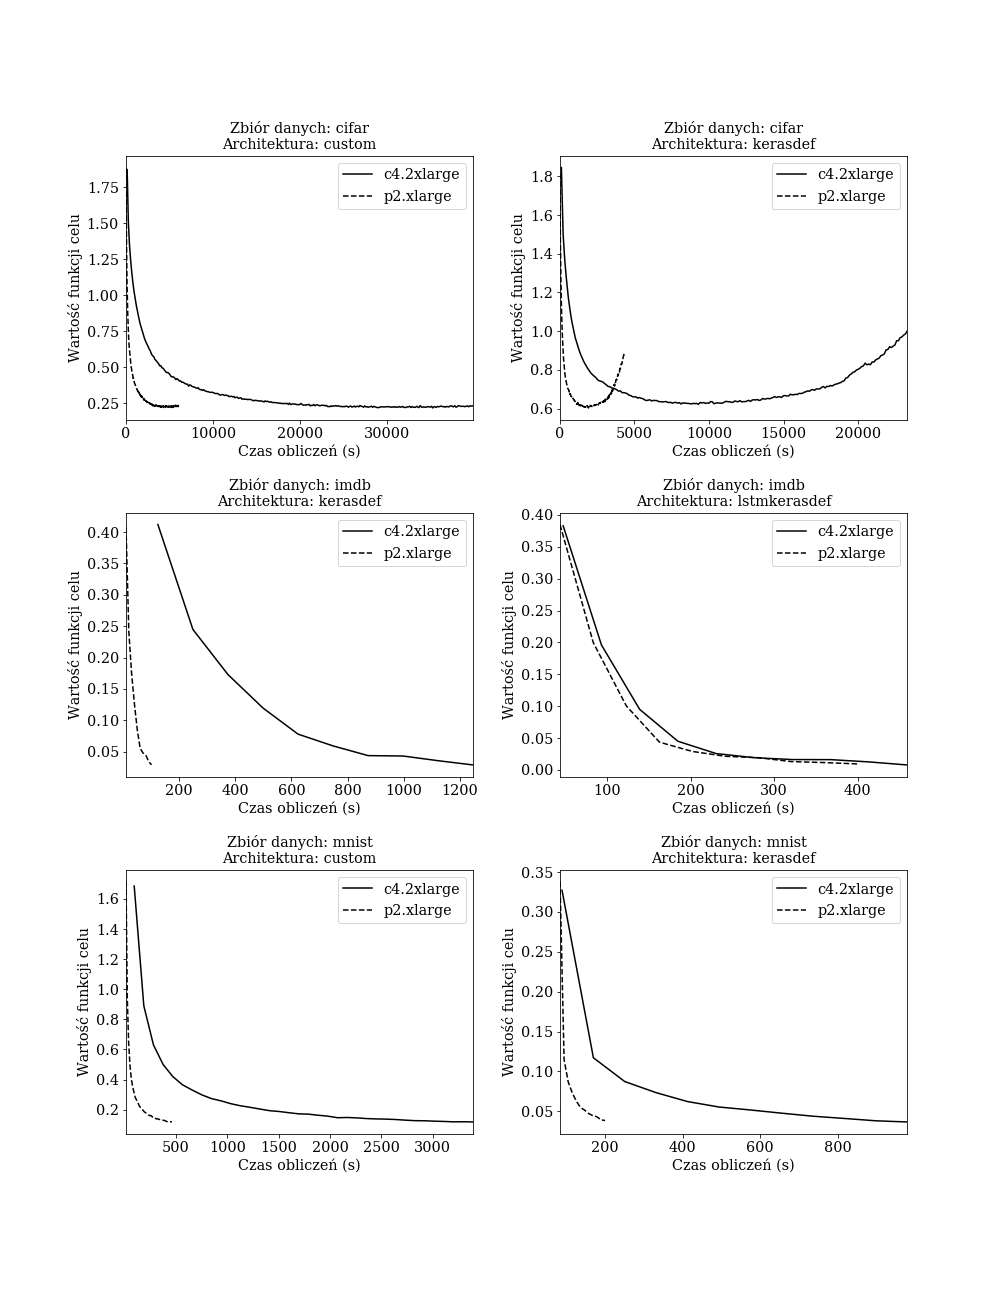
\includegraphics[scale=0.5]{../obrazy/fig:experiment_loss_timecum.png}
\caption{Wykresy wartości funkcji celu dla zbioru treningowego w zależności od czasu obliczeń.\label{fig:experiment_loss_timecum}}
\source{Opracowanie własne.}
\end{figure}
\begin{figure}[h]
  \centering
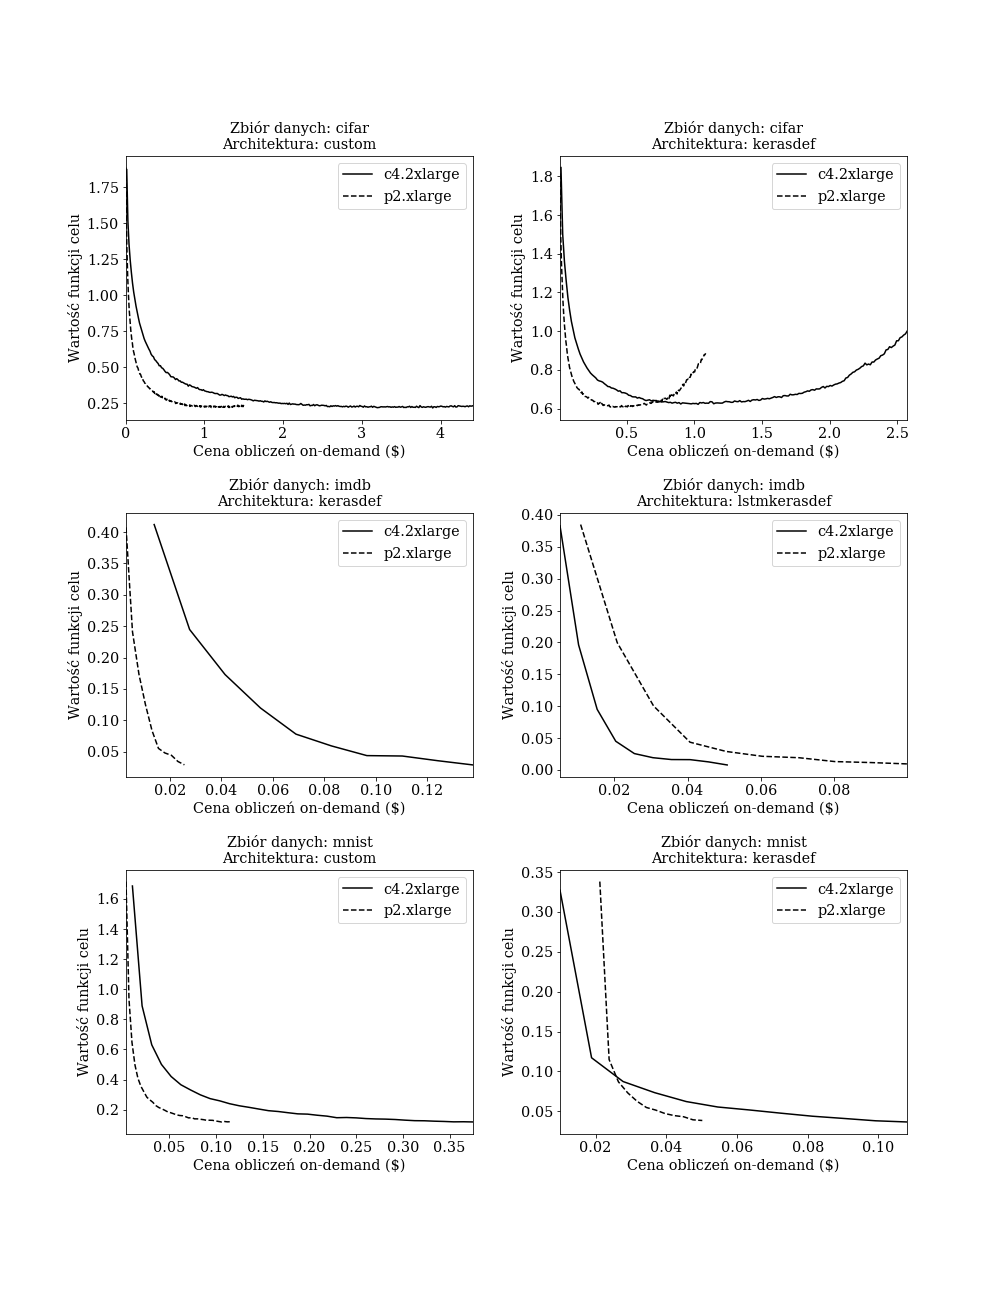
\includegraphics[scale=0.5]{../obrazy/fig:experiment_loss_price_ond.png}
\caption{Wykresy wartości funkcji celu dla zbioru treningowego w zależności od ceny instancji na rynku on-demand.\label{fig:experiment_loss_price_ond}}
\source{Opracowanie własne.}
\end{figure}
\begin{figure}[h]
  \centering
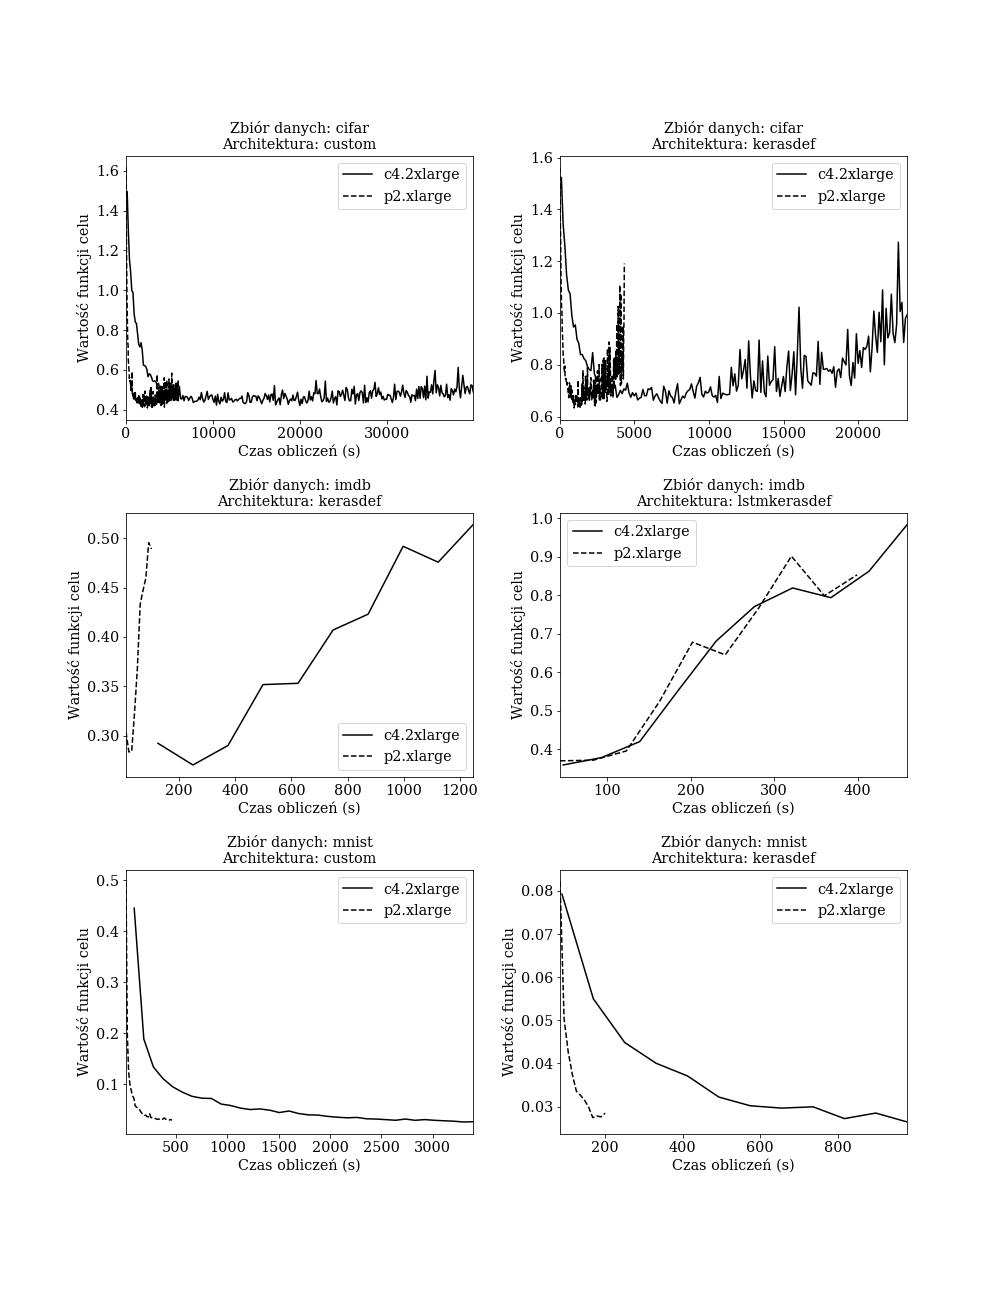
\includegraphics[scale=0.5]{../obrazy/fig:experiment_loss_val_timecum.png}
\caption{Wykresy wartości funkcji celu dla zbioru walidacyjnego w zależności od czasu obliczeń.\label{fig:experiment_loss_val_timecum}}
\source{Opracowanie własne.}
\end{figure}
\begin{figure}[h]
  \centering
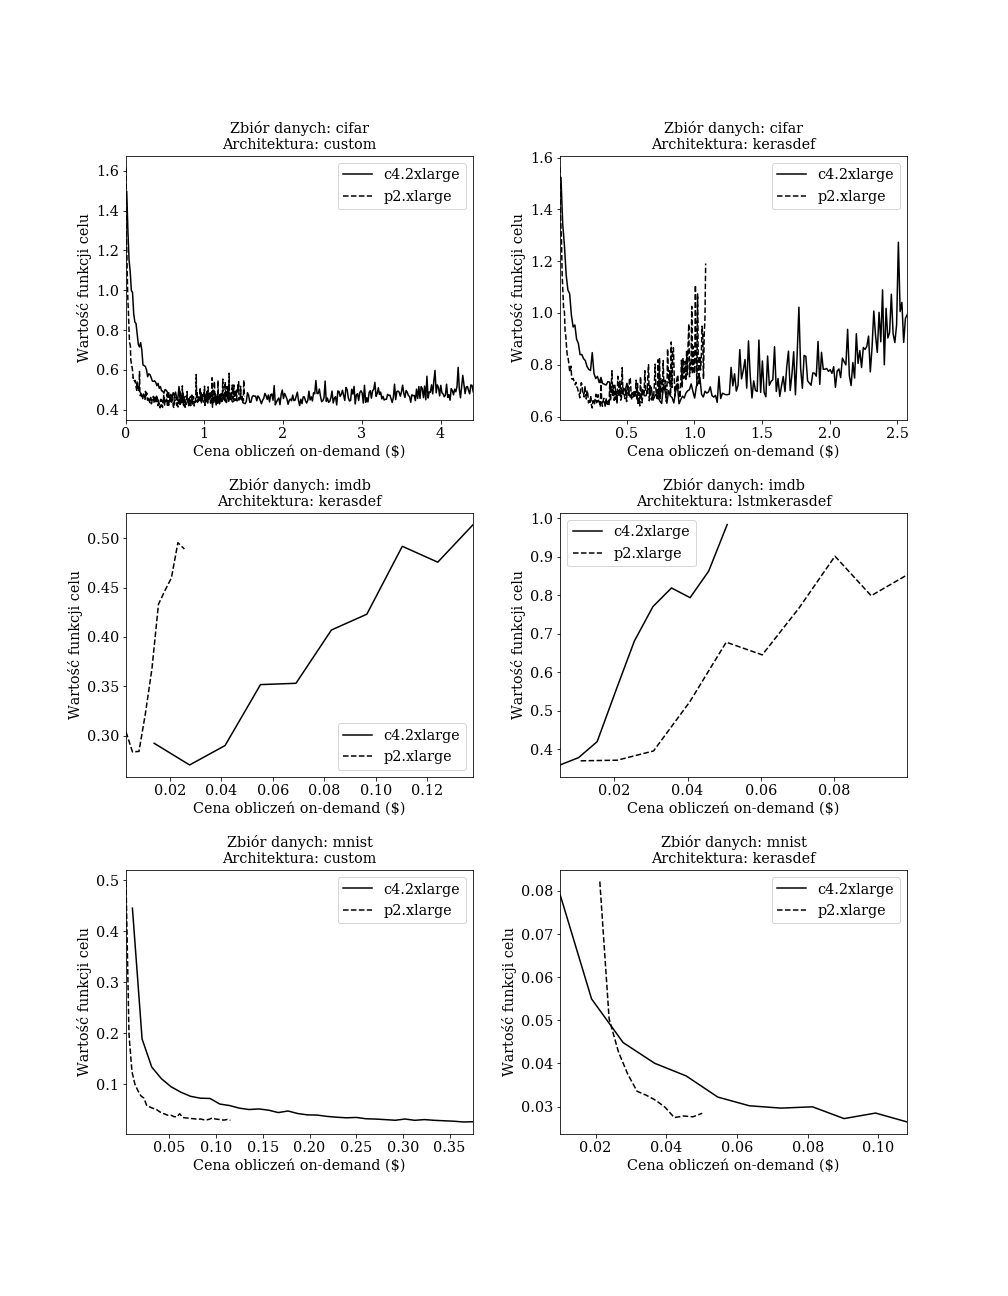
\includegraphics[scale=0.5]{../obrazy/fig:experiment_loss_val_price_ond.png}
\caption{Wykresy wartości funkcji celu dla zbioru walidacyjnego w zależności od ceny instancji na rynku on-demand.\label{fig:experiment_loss_val_price_ond}}
\source{Opracowanie własne.}
\end{figure}
\begin{figure}[h]
  \centering
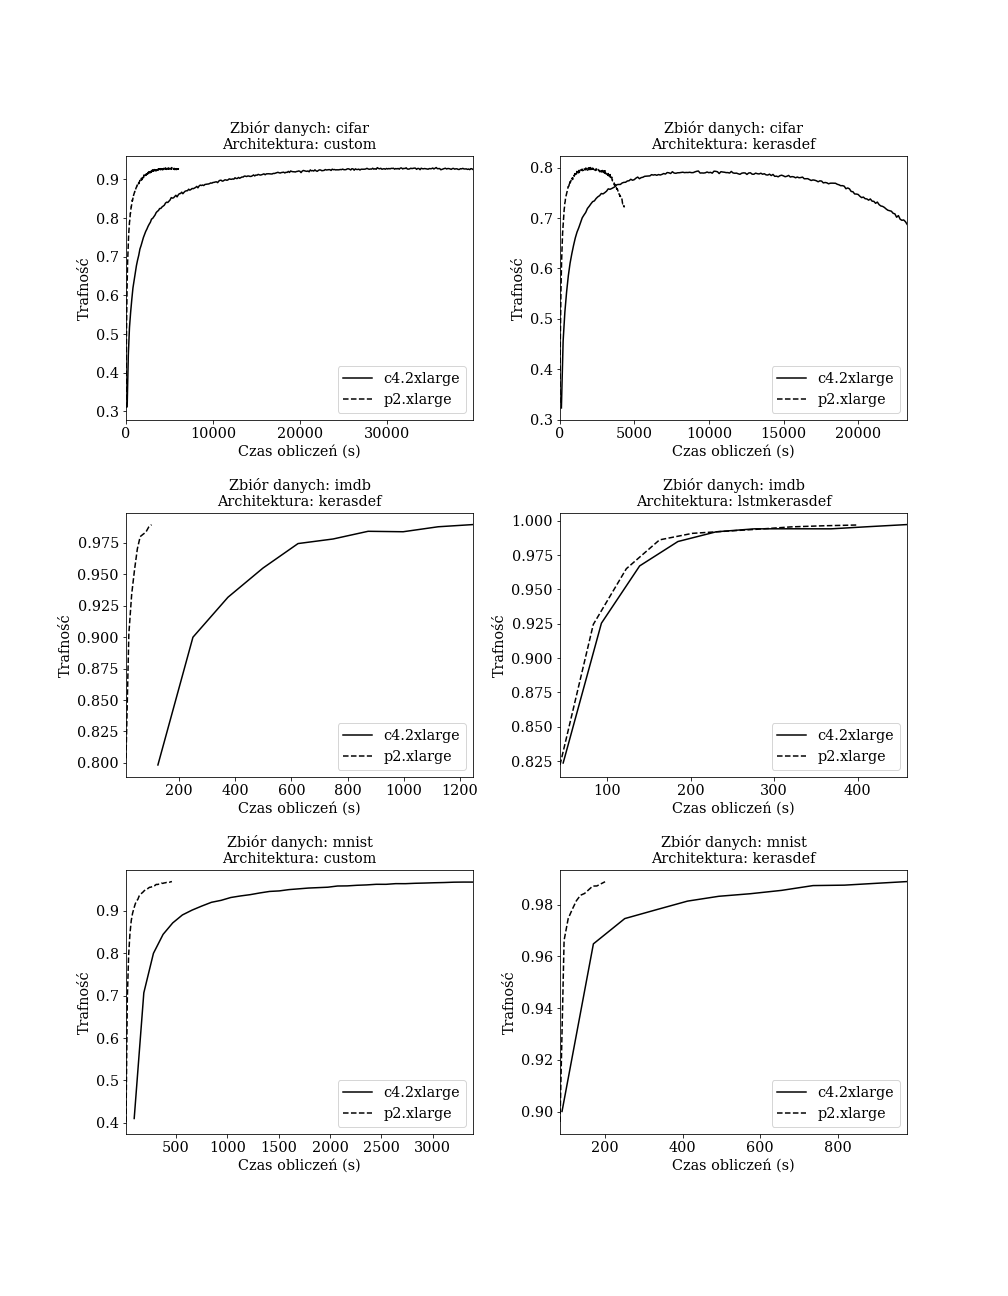
\includegraphics[scale=0.5]{../obrazy/fig:experiment_acc_timecum.png}
\caption{Wykresy trafności dla zbioru treningowego w zależności od czasu obliczeń.\label{fig:experiment_acc_timecum}}
\source{Opracowanie własne.}
\end{figure}
\begin{figure}[h]
  \centering
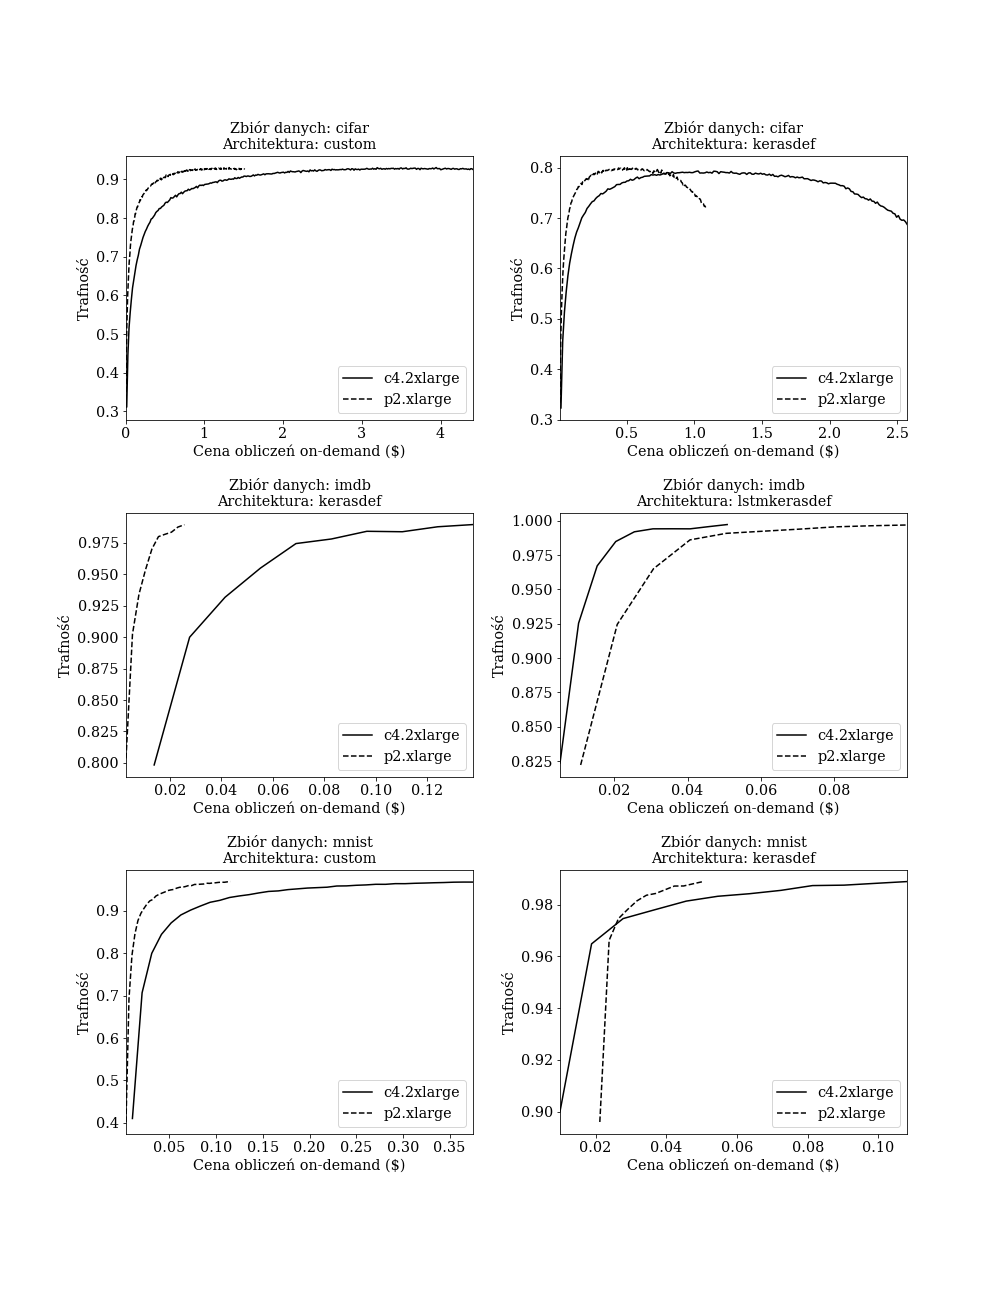
\includegraphics[scale=0.5]{../obrazy/fig:experiment_acc_price_ond.png}
\caption{Wykresy trafności dla zbioru treningowego w zależności od ceny instancji na rynku on-demand.\label{fig:experiment_acc_price_ond}}
\source{Opracowanie własne.}
\end{figure}
\begin{figure}[h]
  \centering
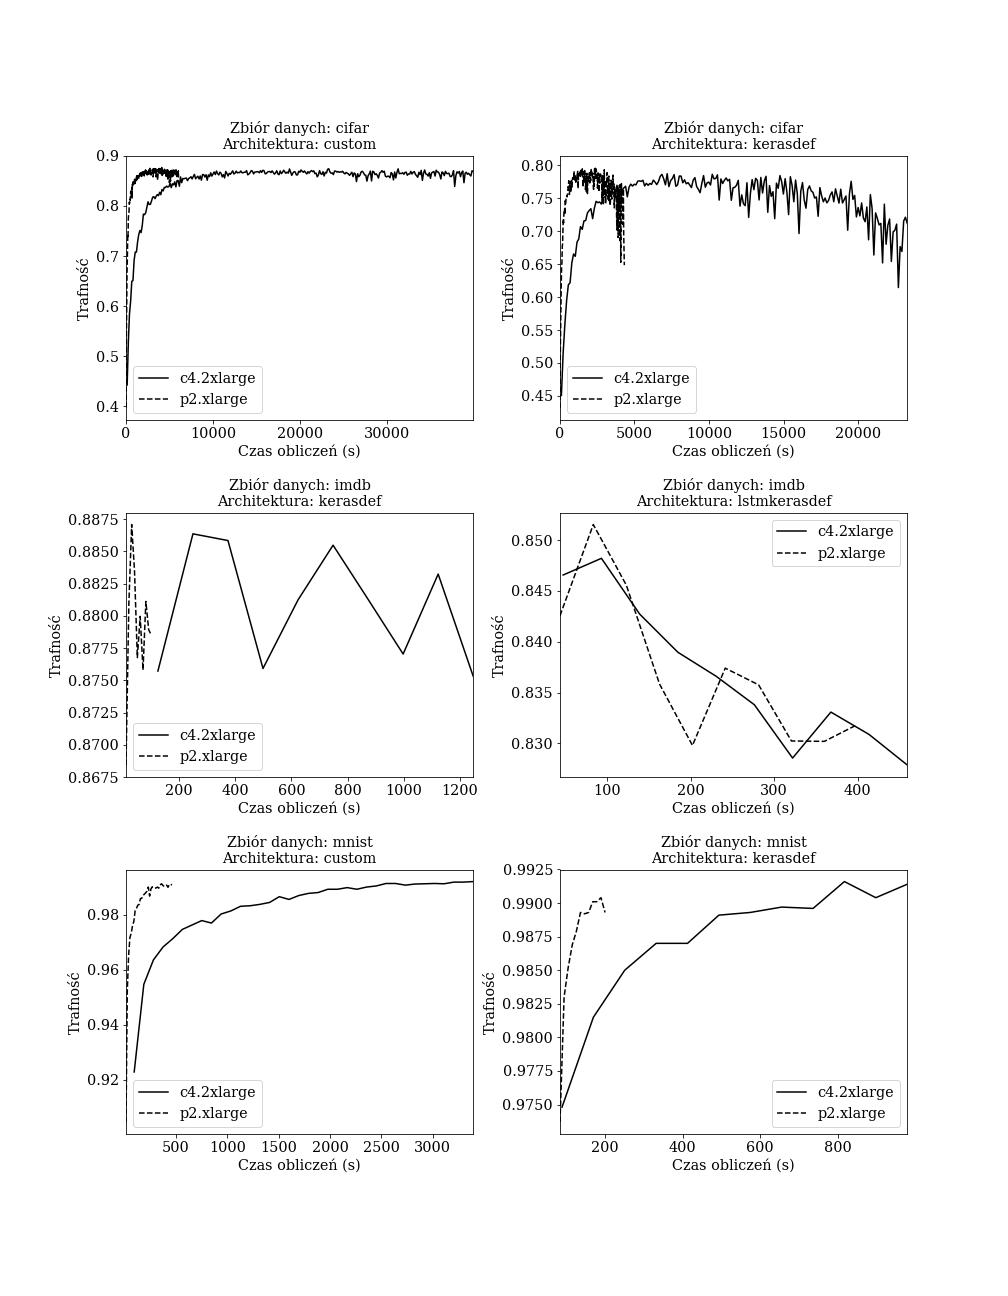
\includegraphics[scale=0.5]{../obrazy/fig:experiment_acc_val_timecum.png}
\caption{Wykresy trafności dla zbioru walidacyjnego w zależności od czasu obliczeń.\label{fig:experiment_acc_val_timecum}}
\source{Opracowanie własne.}
\end{figure}
\begin{figure}[h]
  \centering
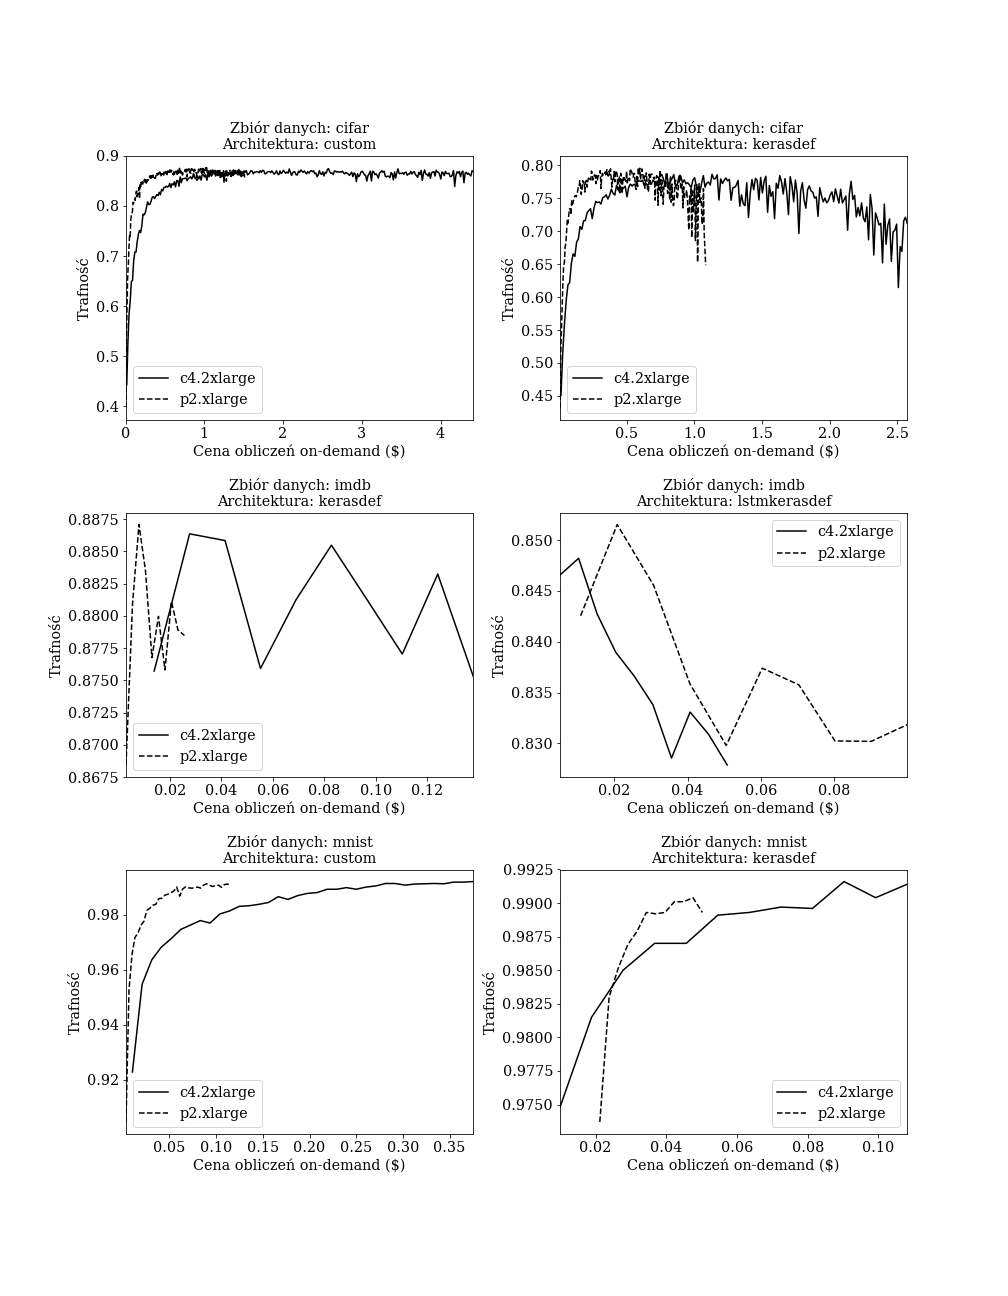
\includegraphics[scale=0.5]{../obrazy/fig:experiment_acc_val_price_ond.png}
\caption{Wykresy trafności dla zbioru walidacyjnego w zależności od ceny instancji na rynku on-demand.\label{fig:experiment_acc_val_price_ond}}
\source{Opracowanie własne.}
\end{figure}

\clearpage

\section{Podsumowanie pracy}

\noindent
W pracy przeprowadzono analizę korzyści płynących z wykorzystywania jednostek posiadających GPU w usługach chmurowych Amazon Web Services. Odpowiedziano na pytanie, czy ich stosowanie jest sposobem na optymalizację kosztową procesu generowania głębokich sieci neuronowychi oraz czy ich większa wydajność rekompensuje wyższą cenę niż w przypadku jednostek nie wyposażonych w procesory graficzne. Dokonano tego przez zrealizowanie eksperymentalnego porównania czasu, nakładu pracy potrzebnego na proces generacji sieci neuronowej i cen wynajmu jednostek obliczeniowych. Wyniki eksperymentu pokazują, że pomimo wyższego kosztu wynajmu instancji GPU za godzinę, zarówno na rynku on-demand, jak i spot, przyśpieszenie procesu uczenia jest na tyle duże, że ich wybór jest rozwiązaniem efektywnym kosztowo względem wykorzystywania instancji bez procesorów graficznych.

Serwery oferowane w ramach usług \textit{cloud computingowych} coraz częściej wykorzystywane są w celu uczenia modeli \textit{machine learningowych} (\citet{calheiros2010}, \citet{github2017}). Przedstawienie narzędzia, służącego do wykonywania \textit{benchmarku} dla dowolnie wybranych jednostek oferowanych w ramach chmury obliczeniowej, dowolnych zbiorów danych i architektur sieci neuronowych ma na celu ułatwić podjęcie decyzji o wyborze serwera i pozwolić na zmierzenie oszczędności względem innych typów jednostek.

Jako kierunki przyszłej pracy można wyznaczyć rozszerzenie eksperymentu zarówno na inne rodzaje zbiorów danych, jak również inne rodzaje architektur. Szczególną uwagę warto poświęcić zadaniom uczenia bez nadzoru, a także rekurencyjnym sieciom neuronowym, które obok sieci konwolucyjnych znajdują obecnie szerokie zastosowanie w rozwiązywaniu problemów \textit{machine learningowych}. Ponadto, istnieje również potrzeba przeprowadzenia podobnego eksperymentu w celu porównania kosztów uczenia modeli na jednostkach oferowanych przez różnych dostawców usług \textit{cloud computingowych}.

\clearpage

\begin{thebibliography}{99}
\setlength{\itemsep}{0pt}%
\bibitem[Abadi et al. (2016)]{abadi2016} Abadi, M., Agarwal, A., Barham, P., Brevdo, E., Chen, Z., Citro, C., \ldots i Ghemawat, S. (2016). Tensorflow: Large-scale machine learning on heterogeneous distributed systems. arXiv preprint arXiv:1603.04467
\bibitem[Akaike (1974)]{akaike1974} Akaike, H. (1974). A new look at the statistical model identification. IEEE transactions on automatic control, 19(6), 716-723
\bibitem[Al-Rhou et al. (2016)]{alrhou2016} Al-Rfou, R., Alain, G., Almahairi, A., Angermueller, C., Bahdanau, D., Ballas, N., \ldots i Bengio, Y. (2016). Theano: A Python framework for fast computation of mathematical expressions. arXiv preprint arXiv:1605.02688
\bibitem[Al-Rfou et al. (2016)]{alrfou2016} Al-Rfou, R., Alain, G., Almahairi, A., Angermueller, C., Bahdanau, D., Ballas, N., \ldots i Bengio, Y. (2016). Theano: A Python framework for fast computation of mathematical expressions. arXiv preprint arXiv:1605.02688
\bibitem[Almeida i Silva (1990)]{almeida1990} Almeida, L. i Silva, F. (1990). Speeding up backpropagation. Adv Neural Comput, 151-158
\bibitem[Anderson i Warrilow (2016)]{anderson2016} Anderson, E. i Warrilow, M. (2016). Market Insight: Cloud Shift — The Transition of IT Spending From Traditional Systems to Cloud. Baza danych Gartner
%\bibitem[Andrychowicz et al. (2016)]{andrychowicz2016} Andrychowicz, M., Denil, M., Gomez, S., Hoffman, M. W., Pfau, D., Schaul, T. i de Freitas, N. (2016). Learning to learn by gradient descent by gradient descent. In Advances in Neural Information Processing Systems, s. 3981-3989
\bibitem[Antonopoulos i Gilliam (2010)]{antonopoulos2010} Antonopoulos, N. i Gillam, L. (2010). Cloud computing, 1st ed. London: Springer
\bibitem[Armburst et al. (2010)]{armburst2010} Armbrust, M., Stoica, I., Zaharia, M., Fox, A., Griffith, R., Joseph, A., Katz, R., Konwinski, A., Lee, G., Patterson, D. i Rabkin, A. (2010). A view of cloud computing. Communications of the ACM, 53(4), s. 50
\bibitem[Baun i Kunze (2011)]{baun2011} Baun, C. i Kunze, M. (2011). Cloud computing. 1st ed. Heidelberg [etc.]: Springer
\bibitem[Bengio i Delalleau (2011)]{bengio2011} Bengio, Y. i Delalleau, O. (2011, October). On the expressive power of deep architectures. In International Conference on Algorithmic Learning Theory (s. 18-36). Springer Berlin Heidelberg
\bibitem[Bengio et al. (2007a)]{bengio2007a} Bengio, Y., Lamblin, P., Popovici, D. i Larochelle, H. (2007a). Greedy layer-wise training of deep networks. Advances in neural information processing systems, 19, 153
\bibitem[Bengio i LeCun (2007b)]{bengio2007b} Bengio, Y. i LeCun, Y. (2007b). Scaling learning algorithms towards AI. Large-scale kernel machines, 34(5), 1-41
\bibitem[Buyya et al. (2009)]{buyya2009} Buyya, R., Yeo, C., Venugopal, S., Broberg, J. i Brandic, I. (2009). Cloud computing and emerging IT platforms: Vision, hype, and reality for delivering computing as the 5th utility. Future Generation Computer Systems, 25(6), s. 599-616
\bibitem[Carr (2008)]{carr2008} Carr, N. G. (2008). The big switch: Rewiring the world, from Edison to Google. WW Norton and Company
\bibitem[Calheiros et al. (2010)]{calheiros2010} Calheiros, R., Ranjan, R., Beloglazov, A., De Rose, C. i Buyya, R. (2010). CloudSim: a toolkit for modeling and simulation of cloud computing environments and evaluation of resource provisioning algorithms. Software: Practice and Experience, 41(1), s. 23-50
\bibitem[Chellapilla et al. (2006)]{chellapilla2006} Chellapilla, K., Puri, S. i Simard, P. (2006). High performance convolutional neural networks for document processing. Tenth International Workshop on Frontiers in Handwriting Recognition. Suvisoft
\bibitem[Chen et al. (2016)]{chen2016} Chen, L. C., Papandreou, G., Kokkinos, I., Murphy, K. i Yuille, A. L. (2016). Deeplab: Semantic image segmentation with deep convolutional nets, atrous convolution, and fully connected crfs. arXiv preprint arXiv:1606.00915
\bibitem[Chen et al. (2015)]{chen2015} Chen, T., Li, M., Li, Y., Lin, M., Wang, N., Wang, M., \ldots i Zhang, Z. (2015). Mxnet: A flexible and efficient machine learning library for heterogeneous distributed systems. arXiv preprint arXiv:1512.01274
\bibitem[Chetlur et al. (2014)]{chetlur2014} Chetlur, S., Woolley, C., Vandermersch, P., Cohen, J., Tran, J., Catanzaro, B. i Shelhamer, E. (2014). cudnn: Efficient primitives for deep learning. arXiv preprint arXiv:1410.0759
\bibitem[Chollet et al. (2015)]{chollet2015} Chollet, F. i inni (2015). Dostępne pod adresem: \url{https://github.com/fchollet/keras} (dostęp 6 czerwca 2017). GitHub
\bibitem[Ciresan et al. (2010)]{ciresan2010} Ciresan, D. C., Meier, U., Gambardella, L. M. i Schmidhuber, J. (2010). Deep big simple neural nets for handwritten digit recogntion. Neural Computation, 22(12):3207–3220.
\bibitem[Ciresan et al. (2011a)]{ciresan2011a} Ciresan, D. C., Meier, U., Masci, J., Gambardella, L. M. i Schmidhuber, J. (2011a). Flexible, high performance convolutional neural networks for image classification. International Joint Conference on Artificial Intelligence IJCAI, s. 1237–1242
\bibitem[Ciresan et al. (2011b)]{ciresan2011b} Ciresan, D. C., Meier, U., Masci, J. i Schmidhuber, J. (2011b). A committee of neural networks for traffic sign classification. International Joint Conference on Neural Networks (IJCNN), s. 1918–1921.
\bibitem[Ciresan et al. (2012)]{ciresan2012} Ciresan, D. C., Giusti, A., Gambardella, L. M. i Schmidhuber, J. (2012). Deep neural networks segment neuronal membranes in electron microscopy images. Advances in Neural Information Processing Systems (NIPS), s. 2852–2860
\bibitem[Ciresan i Schmidhuber (2013)]{ciresan2013} Ciresan, D. C. and Schmidhuber, J. (2013). Multi-column deep neural networks for offline handwritten Chinese character classification. Technical report, IDSIA. arXiv:1309.0261
\bibitem[Collobert et al. (2011)]{collobert2011} Collobert, R., Kavukcuoglu, K. i Farabet, C. (2011). Torch7: A matlab-like environment for machine learning. In BigLearn, NIPS Workshop (nr EPFL-CONF-192376)
\bibitem[Edwards (1993)]{edwards1993} Edwards, P. J. (1993). Synaptic weight noise during MLP learning enhances fault-tolerance, generalisation and learning trajectory
\bibitem[Forbes.com (2017)]{forbes2017} Forbes.com. (2017). Amazon Continues To Gain Share In Cloud Infrastructure Services Market. Dostępne pod adresem: \url{https://www.forbes.com/sites/greatspeculations/2016/08/17/amazon-continues-to-gain-share-in-cloud-infrastructure-services-market/#2277485215b8} (dostęp 11 marca 2017)
\bibitem[Fukushima (1975)]{fukushima1975} Fukushima, K. (1975). Cognitron: A self-organizing multilayered neural network. Biological cybernetics, 20(3-4), 121-136
\bibitem[Fukushima (1980)]{fukushima1980} Fukushima, K. (1980). Neocognitron: A self-organizing neural network for a mechanism of pattern recognition unaffected by shift in position. Biological Cybernetics, 36(4):193–202
\bibitem[Girshick et al. (2014)]{girschick2014} Girshick, R., Donahue, J., Darrell, T. i Malik, J. (2014). Rich feature hierarchies for accurate object detection and semantic segmentation. In Proceedings of the IEEE conference on computer vision and pattern recognition, s. 580-587
\bibitem[Github (2017)]{github2017} GitHub. (2017). Benchmarks for popular convolutional neural network models on CPU and different GPUs, with and without cuDNN. Dostępne pod adresem: \url{https://github.com/jcjohnson/cnn-benchmarks} (dostęp 14 marca 2017)
\bibitem[Goldberg (1974)]{goldberg1974} Goldberg, R. P. (1974). Survey of virtual machine research. IEEE Comput Mag 7(6):34–45
\bibitem[Goldberg i Levy (2014)]{goldberg2014} Goldberg, Y. i Levy, O. (2014). word2vec explained: Deriving mikolov et al.'s negative-sampling word-embedding method. arXiv preprint arXiv:1402.3722
\bibitem[Goodfellow et al. (2016)]{goodfellow2016} Goodfellow, I., Bengio, Y. i Courville, A. (2016). Deep Learning. MIT Press
\bibitem[Graves i Schmidhuber (2005)]{graves2005} Graves, A. i Schmidhuber, J. (2005). Framewise phoneme classification with bidirectional LSTM and other neural network architectures. Neural Networks, 18(5), 602-610
\bibitem[Gysel (2016)]{gysel2016} Gysel P. M. (2016). Ristretto: Hardware-Oriented Approximation of Convolutional Neural Networks. arXiv preprint arXiv:1605.06402
\bibitem[Hacker Noon (2017)]{hackernoon2017} Hacker Noon. (2017). GPUs and Kubernetes for Deep Learning. Dostępne pod adresem: \url{https://hackernoon.com/gpus-kubernetes-for-deep-learning-part-1-3-d8eebe0dd6fe#.jn1xjvpd2} (dostęp 14 marca 2017)
%\bibitem[Han et al. (2015)]{han2015} Han, S., Mao, H. i Dally, W. J. (2015). Deep compression: Compressing deep neural networks with pruning, trained quantization and huffman coding. arXiv preprint arXiv:1510.00149
\bibitem[Han et al. (2016)]{han2016} Han, S., Liu, X., Mao, H., Pu, J., Pedram, A., Horowitz, M. A. i Dally, W. J. (2016) EIE: Efficient Inference Engine on Compressed Deep Neural Network. arXiv preprint arXiv:1602.01528, 2016a
\bibitem[Hanson (1990)]{hanson1990} Hanson, S. J. (1990). A stochastic version of the delta rule. Physica D: Nonlinear Phenomena, 42(1-3), 265-272
\bibitem[Hastie i Tibshirani (1990)]{hastie1990} Hastie, T. J. i Tibshirani, R. J. (1990). Generalized additive models (tom 43). CRC press
\bibitem[Hebb (1949)]{hebb1949} Hebb, D.O. (1949). The Organization of Behavior. New York: Wiley and Sons
\bibitem[Hecht-Nielsen (1988)]{hecht1988} Hecht-Nielsen, R. (1988). Theory of the backpropagation neural network. Neural Networks, 1, s. 445
\bibitem[Hinton i Sejnowski (1986)]{hinton1986} Hinton, G. E. i Sejnowski, T. J. (1986). Learning and relearning in Boltzmann Machines. Parallel Distributed Processing, Rumelhart et al, Eds
\bibitem[Hinton i Van Camp (1993)]{hinton1993} Hinton, G. E. i Van Camp, D. (1993, August). Keeping the neural networks simple by minimizing the description length of the weights. Proceedings of the sixth annual conference on Computational learning theory (s. 5-13). ACM
\bibitem[Hinton (2006a)]{hinton2006a} Hinton, G. (2006a). Reducing the Dimensionality of Data with Neural Networks. Science, 313(5786), s. 504-507
\bibitem[Hinton et al. (2006b)]{hinton2006b} Hinton, G., Osindero, S. i Teh, Y. (2006b). A Fast Learning Algorithm for Deep Belief Nets. Neural Computation, 18(7), s. 1527-1554
\bibitem[Hinton et al. (2012)]{hinton2012} Hinton, G., Deng, L., Yu, D., Dahl, G., Mohamed, A., Jaitly, N., Senior, A., Vanhoucke, V., Nguyen, P., Sainath, T. i Kingsbury, B. (2012). Deep Neural Networks for Acoustic Modeling in Speech Recognition: The Shared Views of Four Research Groups. IEEE Signal Processing Magazine, 29(6), s. 82-97
\bibitem[Hochreiter (1991)]{hochreiter1991} Hochreiter, S. (1991). Untersuchungen zu dynamischen neuronalen Netzen. Diploma thesis, Institut für Informatik, Lehrstuhl Prof. Brauer, Technische Universität München. Advisor: J. Schmidhuber
\bibitem[Hochreiter i Schmidhuber (1997)]{hochreiter1997} Hochreiter, S. i Schmidhuber, J. (1997). Long short-term memory. Neural computation, 9(8), s. 1735-1780
\bibitem[Igel i Husken (2003)]{igel2003} Igel, C. i Hüsken, M. (2003). Empirical evaluation of the improved Rprop learning algorithms. Neurocomputing, 50, s. 105-123
\bibitem[Ivakhnenko i Lapa (1965)]{ivakhnenko1965} Ivakhnenko, A. G. i Lapa, V. G. (1965). Cybernetic Predicting Devices. CCM Information Corporation
\bibitem[Ivakhnenko i Lapa (1967)]{ivakhnenko1967} Ivakhnenko, A. G., Lapa, V. G., and McDonough, R. N. (1967). Cybernetics and forecasting techniques. American Elsevier, NY
\bibitem[Ivakhnenko i Lapa (1968)]{ivakhnenko1968} Ivakhnenko, A. G. (1968). The group method of data handling-a rival of the method of stochastic approximation. Soviet Automatic Control, 13(3), 43-55
\bibitem[Jacobs (1989)]{jacobs1989} Jacobs, R. A. (1988). Increased rates of convergence through learning rate adaptation. Neural networks, 1(4), 295-307
\bibitem[Jain i Seung (2009)]{jain2009} Jain, V. i Seung, S. (2009). Natural image denoising with convolutional networks. Koller, D., Schuurmans, D., Bengio, Y., and Bottou, L., editors, Advances in Neural Information Processing Systems (NIPS) 21, s. 769–776. Curran Associates, Inc.
\bibitem[Jermain et al. (2015)]{jermain2015} Jermain, C. L., Rowlands, G. E., Buhrman, R. A., i Ralph, D. C. (2015). GPU-accelerated micromagnetic simulations using cloud computing. arXiv preprint arXiv:1505.01207
\bibitem[Jia et al. (2014)]{jia2014} Jia, Y., Shelhamer, E., Donahue, J., Karayev, S., Long, J., Girshick, R., \ldots i Darrell, T. (2014). Caffe: Convolutional architecture for fast feature embedding. Proceedings of the 22nd ACM international conference on Multimedia (s. 675-678). ACM
\bibitem[Kingma i Ba (2014)]{kingma2014} Kingma, D. i Ba, J. (2014). Adam: A method for stochastic optimization. arXiv preprint arXiv:1412.6980
\bibitem[Kleinrock (2005)]{kleinrock2005} Kleinrock, L., A Vision for the Internet. ST Journal for Research, tom 2, nr 1, s. 4–5
\bibitem[Krizhevsky i Hinton (2009)]{krizhevsky2009} Krizhevsky, A. i Hinton, G. (2009). Learning multiple layers of features from tiny images
\bibitem[Krizhevsky et al. (2012)]{krizhevsky2012} Krizhevsky, A., Sutskever, I. i Hinton, G. (2012). Imagenet classification with deep convolutional neural networks. In Advances in neural information processing systemsk, s. 1097-1105
\bibitem[LeCun et al. (1989)]{lecun1989a} LeCun, Y., Denker, J. S., Solla, S. A., Howard, R. E., Jackel, L. D. (1989, November). Optimal brain damage. NIPs (tom 2, s. 598-605).
\bibitem[LeCun et al. (1989)]{lecun1989b} LeCun, Y., Boser, B., Denker, J. S., Henderson, D., Howard, R. E., Hubbard, W. i Jackel, L. D. (1989). Backpropagation applied to handwritten zip code recognition. Neural computation, 1(4), 541-551
\bibitem[LeCun et al. (1998)]{lecun1998} LeCun, Y., Bottou, L. , Bengio, Y. i Haffner, P. (1998). Gradient-based learning applied to document recognition. Proceedings of the IEEE, 86(11):2278-2324
\bibitem[LeCun, Bengio i Hinton (2015)]{lecun2015} LeCun, Y., Bengio, Y. i Hinton, G. (2015). Deep learning. Nature, 521(7553), s.436-444
\bibitem[Leong et al. (2017)]{leong2017} Leong, L., Petri, G., Gill, B. i Dorosh, M. (2017). Magic Quadrant for Cloud Infrastructure as a Service. Gartner.com. Dostępne pod adresem: \url{https://www.gartner.com/doc/reprints?id=1-2G2O5FC&ct=150519} (dostęp 11 marca 2017)
\bibitem[Linnainmaa (1970)]{linnainmaa1970} Linnainmaa, S. (1970). The representation of the cumulative rounding error of an algorithm as a
Taylor expansion of the local rounding errors. Praca magisterska, Uniwersytet w Helsinkach
\bibitem[Litvinenko (2014)]{litvinenko2014} Litvinenko, N. (2014). Using of GPUs for cluster analysis of large data by K-means method arXiv preprint arXiv:1402.3788
\bibitem[Maas et al. (2011)]{maas2011} Maas, A. L., Daly, R. E., Pham, P. T., Huang, D., Ng, A. Y. i Potts, C. (2011). Learning word vectors for sentiment analysis. In Proceedings of the 49th Annual Meeting of the Association for Computational Linguistics: Human Language Technologies-Volume 1 (s. 142-150). Association for Computational Linguistics
\bibitem[Mackay (1992)]{mackay1992} MacKay, D. J. (1992). A practical Bayesian framework for backpropagation networks. Neural computation, 4(3), 448-472
\bibitem[McCulloch i Pitts (1943)]{mcculloch1943} McCulloch, W. S. i Pitts, W. (1943). A logical calculus of the ideas immanent in nervous activity. The bulletin of mathematical biophysics, 5(4), s. 115-133
\bibitem[Medium (2017a)]{medium2017a} Medium (2017). TensorFlow 1.0 is here. Let’s do some Deep Learning on the Amazon Cloud! – Sigmoidal. Dostępne pod adresem: \url{https://medium.com/sigmoidal/tensorflow-1-0-is-here-lets-do-some-deep-learning-on-the-amazon-cloud-9234eab31fa5#.vyxzk4bwk} (dostęp 14 marca 2017)
\bibitem[Medium (2017b)]{medium2017b} Medium (2017). Keras with GPU on Amazon EC2 – a step-by-step instruction. Dostępne pod adresem: \url{https://medium.com/@mateuszsieniawski/keras-with-gpu-on-amazon-ec2-a-step-by-step-instruction-4f90364e49ac#.i2rxriv4g} (dostęp 14 marca 2017)
\bibitem[Mell i Grance (2011)]{mell2011} Mell, P. i Grance T. (2011). The NIST definition of cloud computing
\bibitem[Menon et al. (2005)]{menon2005} Menon, A., Santos, J., Turner, Y., Janakiraman, G. i Zwaenepoel, W. (2005). Diagnosing performance overheads in the xen virtual machine environment. Proceedings of the 1st ACM/USENIX international conference on Virtual execution environments - VEE '05
\bibitem[Minsky i Papert (1969)]{minsky1969} Minsky, M. i Papert, S. (1969). Perceptrons. Cambridge, MA: MIT Press
\bibitem[Misra et al. (2016)]{misra2016} Misra, I., Lawrence Zitnick, C., Mitchell, M. i Girshick, R. (2016). Seeing through the Human Reporting Bias: Visual Classifiers from Noisy Human-Centric Labels. In Proceedings of the IEEE Conference on Computer Vision and Pattern Recognition (s. 2930-2939)
\bibitem[Mnih et al. (2013)]{mnih2013} Mnih, V., Kavukcuoglu, K., Silver, D., Graves, A., Antonoglou, I., Wierstra, D. i Riedmiller, M. (2013). Playing atari with deep reinforcement learning. arXiv preprint arXiv:1312.5602
\bibitem[Moody (1991)]{moody1991} Moody, J. E. (1991, December). The effective number of parameters: An analysis of generalization and regularization in nonlinear learning systems. In NIPS (tom 4, s. 847-854)
\bibitem[Moody i Utans (1994)]{moody1994} Moody, J., i Utans, J. (1994). Architecture selection strategies for neural networks: Application to corporate bond rating prediction. In Neural networks in the capital markets (pp. 277-300). John Wiley \& Sons.
\bibitem[Mustafa et al. (2015)]{mustafa2015} Mustafa, S., Nazir, B., Hayat, A., Khan, A. i Madani, S. (2015). Resource management in cloud computing: Taxonomy, prospects, and challenges. Computers and Electrical Engineering, 47, s. 186-203
\bibitem[Nowlan i Hinton (1992)]{nowlan1992} Nowlan, S. J. i Hinton, G. E. (1992). Simplifying neural networks by soft weight-sharing. Neural computation, 4(4), 473-493
\bibitem[OECD (2014)]{oecd2014} OECD (2014). Cloud Computing: The Concept, Impacts and the Role of Government Policy. OECD Digital Economy Papers, No. 240, OECD Publishing, Paris
\bibitem[Oh i Jung (2004)]{oh2004} Oh, K. S. i Jung, K. (2004). GPU implementation of neural networks. Pattern Recognition, 37(6), 1311-1314
\bibitem[Ranzato et al. (2006)]{ranzato2006} Ranzato, M., Poultney, C., Chopra, S. i LeCun, Y. (2006). Efficient learning of sparse representations with an energy-based model. In et al., J. P., editor, Advances in Neural Information Processing Systems (NIPS 2006). MIT Press
\bibitem[Ranzato et al. (2007)]{ranzato2007} Ranzato, M. A., Huang, F., Boureau, Y. i LeCun, Y. (2007). Unsupervised learning of invariant feature hierarchies with applications to object recognition. Proc. Computer Vision and Pattern Recognition Conference (CVPR’07), s. 1–8. IEEE Press
\bibitem[Riedmiller i Braun (1993)]{riedmiller1993} Riedmiller, M. i Braun, H. (1993). A direct adaptive method for faster backpropagation learning: The RPROP algorithm. In Neural Networks, 1993., IEEE International Conference on (s. 586-591). IEEE
\bibitem[Rosenblatt (1957)]{rosenblatt1957} Rosenblatt, F. (1957). The Perceptron--a perceiving and recognizing automaton. Report 85-460-1, Cornell Aeronautical Laboratory
\bibitem[Rumelhart et al. (1986)]{rumelhart1986} Rumelhart, D. E., Hinton, G. E. i Williams, R. J. (1986). Learning representations by back-propagating errors. Nature, 323, 533-536
\bibitem[Schuster (1997)]{schuster1997} Schuster, M. i Paliwal, K. K. (1997). Bidirectional recurrent neural networks. IEEE Transactions on Signal Processing, 45(11), s. 2673-2681
\bibitem[Schmidhuber i Hochreiter (1997)]{schmidhuber1997} Schmidhuber, J. i Hochreiter, S. (1997). Long short-term memory. Neural Comput, 9(8), s. 1735-1780
\bibitem[Schmidhuber (2015)]{schmidhuber2015} Schmidhuber, J. (2015). Deep learning in neural networks: An overview. Neural networks, 61, 85-117
\bibitem[Shetty (2016)]{shetty2016} Shetty, S. (2016).  Application of Convolutional Neural Network for Image Classification on Pascal VOC Challenge 2012 dataset. arXiv preprint arXiv:1607.03785
\bibitem[Shi et al. (2016)]{shi2016} Shi, S., Wang, Q., Xu, P. i Chu, X. (2016). Benchmarking State-of-the-Art Deep Learning Software Tools. arXiv preprint arXiv:1608.07249
\bibitem[Shroff (2010)]{shroff2010} Shroff, G. (2010). Enterprise cloud computing. 1st ed. Cambridge: Cambridge University Press
\bibitem[Smith et al. (2009)]{smith2009} Smith D. M. et al. (2009). Hype Cycle for Cloud Computing (ID: G00168780). Baza danych Gartner
\bibitem[Smolensky (1986)]{smolensky1986} Smolensky, P. (1986). Parallel distributed processing: Explorations in the microstructure of cognition, tom 1. Information Processing in Dynamical Systems: Foundations of Harmony Theory. MIT Press, Cambridge, MA, USA, 15, 18
\bibitem[Srivastava et al. (2014)]{srivastava2014} Srivastava, N., Hinton, G. E., Krizhevsky, A., Sutskever, I. i Salakhutdinov, R. (2014). Dropout: a simple way to prevent neural networks from overfitting. Journal of Machine Learning Research, 15(1), s. 1929-1958
\bibitem[Strom (2015)]{strom2015} Strom, N. (2015). Scalable distributed DNN training using commodity GPU cloud computing. INTERSPEECH (tom 7, s. 10)
\bibitem[Szegedy (2014)]{szegedy2014} Szegedy, C. et al. (2014). Going deeper with convolutions. arXiv preprint arXiv:1409.4842
\bibitem[Tadeusiewicz (1993)]{tadeusiewicz1993} Tadeusiewicz, R. (1993). Sieci neuronowe. Akademicka Oficyna Wydawnicza RM, s. 13
\bibitem[Tieleman i Hinton (2012)]{tieleman2012} Tieleman, T. i Hinton, G. (2012). Lecture 6.5-rmsprop: Divide the gradient by a running average of its recent magnitude. COURSERA: Neural networks for machine learning, 4(2)
\bibitem[Touretzky i Hinton (1985)]{touretzky1985} Touretzky, D. S. i Hinton, G. E. (1985, August). Symbols among the neurons: Details of a connectionist inference architecture. In IJCAI (tom 85, s. 238-243)
\bibitem[Vanhoucke et al. (2011)]{vanhoucke2011} Vanhoucke, V., Senior, A. i Mao, M. Z. (2011). Improving the speed of neural networks on CPUs. In Proc. Deep Learning and Unsupervised Feature Learning NIPS Workshop (tom 1, s. 4)
\bibitem[Wan (1993)]{wan1993} Wan, E.A., 1993. Time series prediction by using a connectionist network with internal delay lines. Santa Fe Institute Studies in the sciences of complexity-proceedings volume (tom 15, s. 195-195). Addison-Wesley publishing co.
\bibitem[Ward i Baker (2013)]{ward2013} Ward, J.S. i Barker, A. (2013). A Cloud Computing Survey: Developments and Future Trends in Infrastructure as a Service Computing
\bibitem[Wenge et al. (1992)]{weng1992} Weng, J., Ahuja, N. i Huang, T. S. (1992, June). Cresceptron: a self-organizing neural network which grows adaptively. In Neural Networks, 1992. IJCNN., International Joint Conference on (Vol. 1, pp. 576-581). IEEE
\bibitem[Widrow i Hoff (1960)]{widrow1960} Widrow, B. i Hoff, M. E. (1960, August). Adaptive switching circuits. In IRE WESCON convention record (tom 4, nr 1, s. 96-104)
\bibitem[Yang et al. (2009)]{yang2009} Yang, M., Ji, S., Xu, W., Wang, J., Lv, F., Yu, K., Gong, Y., Dikmen, M., Lin, D. J. i Huang, T. S. (2009). Detecting human actions in surveillance videos. In TREC Video Retrieval Evaluation Workshop
\bibitem[Yu et al. (2014)]{yu2014} Yu, D., Eversole, A., Seltzer, M., Yao, K., Huang, Z., Guenter, B., \ldots i Droppo, J. (2014). An introduction to computational networks and the computational network toolkit. Microsoft Technical Report MSR-TR-2014–112
\bibitem[Zeiler (2012)]{zeiler2012} Zeiler, M. D. (2012). ADADELTA: an adaptive learning rate method. arXiv preprint arXiv:1212.5701
\bibitem[Zhang et al. (2010)]{zhang2010} Zhang, Q., Cheng, L. i Boutaba, R. (2010). Cloud computing: state-of-the-art and research challenges. Journal of Internet Services and Applications, 1(1), s. 7-18

\end{thebibliography}
\clearpage

\listoffigures

\clearpage

\listoftables

\clearpage

\begin{appendices}

\section{Eksperyment}

\subsection{Kod sterujący}

\begin{lstlisting}[language=python]

  import boto3, subprocess
  import datetime
  import time
  import argparse
  import fabric
  from fabric.api import run, hide

  def parseArgs():
      parser = argparse.ArgumentParser(description='Experiment specs')
      parser.add_argument('--instance_type', type=str, help='instance type')
      return  parser.parse_args()

  class benchmark:
      def __init__(self, experiments, instance_type, image_id="ami-a3b3d4b5", key_name='dpcld_test1'):
          self.experiments = experiments
          self.instance_type = instance_type
          self.image_id = image_id
          self.key_name = key_name
          self.run_date = datetime.date.strftime(datetime.date.today(), '%Y%m%d')
          self.client = boto3.client('ec2')
          self.ec2 = boto3.resource('ec2')
          self.p_ids = dict()

      def setUpInstances(self):

          response = self.client.run_instances(ImageId=self.image_id,
                                  InstanceType=self.instance_type,
                                  MinCount=1,
                                  MaxCount=1,
                                  KeyName=self.key_name,
                                  IamInstanceProfile={
                                      'Arn':'arn:aws:iam::465729247037:instance-profile/S3_Admin_Access'}
                                  )

          assert response.get('ResponseMetadata').get('HTTPStatusCode') == 200, "Request ended with an error (HTTPStatusCode != 200)"
          assert len(response.get('Instances')) == 1, "Number of instances launched is equal to specified"

          instance_ids = []
          instance_ids.extend([_.get('InstanceId') for _ in response.get('Instances')])

          waiter = self.client.get_waiter('instance_status_ok')
          waiter.wait(InstanceIds=instance_ids)

          print('Set up instances: {}'.format(' '.join(instance_ids)))

          self.instances = [self.ec2.Instance(_) for _ in instance_ids]

          #return [self.ec2.Instance(_) for _ in instance_ids]

      def configureInstances(self):
          [self.configureInstance(i, e) for i, e in zip(self.instances, self.experiments)]

      def configureInstance(self, instance, experiment):
          instance.create_tags(Tags=[{'Key':'Name', 'Value':'sequential experiment'}])
          fabric.api.env.host_string = 'ec2-user@{}'.format(instance.public_dns_name)
          fabric.api.env.key_filename = '~/.ssh/{}.pem'.format(self.key_name)
          fabric.api.env.disable_known_hosts
          fabric.api.hide('output')
          fabric.operations.put('./{}_{}.py'.format(*experiment), '.')
          run('sudo pip3 install git+git://github.com/fchollet/keras.git --upgrade')
          run('sudo pip3 install pydot')
          run('sudo pip3 install graphviz')

      def runExperiments(self):
          [self.runExperiment(i, e) for i, e in zip(self.instances, self.experiments)]

      def runExperiment(self, instance, experiment):
          fabric.api.env.host_string = 'ec2-user@{}'.format(instance.public_dns_name)
          run('mkdir -p logs')
          run('nohup python3 -u {0}_{1}.py \
          --run_date {2} --dataset {0} --architecture {1} --instance_type {3} \
          >logs/{2}_{0}_{1}_{3}.log 2>logs/{2}_{0}_{1}_{3}.err < /dev/null &'
              .format(*experiment, self.run_date, self.instance_type), pty=False)
          self.p_ids[instance.id] = run('pgrep python3')

      def getExperimentLogs(self):

          while True:
              instance = self.instances[0]
              fabric.api.env.host_string = 'ec2-user@{}'.format(instance.public_dns_name)

              status = benchmark_td1.client.describe_instance_status(InstanceIds=[instance.id])\
              .get('InstanceStatuses')[0]\
              .get('InstanceState')\
              .get('Name')

              if status != 'running':
                  print('Instance {} not running'.format(instance.id))
                  break

              self.rSync(instance.public_dns_name)
              self.syncWithS3()

              try:
                  run('pgrep python3')
              except:
                  print('Process on instance {} not found'.format(instance.id))
                  break

              time.sleep(60)

              print('{}: synchronized logs from all instances'.format(datetime.datetime.now().isoformat()))
          else:
              print('All instances are down or finished their tasks')

      def rSync(self, public_dns):
          fabric.operations.local('rsync -aL -e "ssh -i ~/.ssh/{}.pem -o StrictHostKeyChecking=no" \
          --include="/home/ec2-user/logs/*" --include="*.log" --include="*.err" \
          --include="*.out" --include="*.png" --exclude="*" \
          ec2-user@{}:/home/ec2-user/logs/ \
          ./logs/'.format(self.key_name, public_dns))

      def syncWithS3(self):
          run('aws s3 sync /home/ec2-user/logs s3://deepcloud-logstash/ --exclude="*"\
          --include="*.log" --include="*.err" \
          --include="*.out" --include="*.png" --region "us-east-1"')

  if __name__ == "__main__":
      experiments = [("mnist","kerasdef"),
                     ("mnist","custom"),
                     ("imdb","kerasdef"),
                     ("imdb","lstmkerasdef"),
                     ("cifar","kerasdef"),
                     ("cifar","custom")
                     ]
      args = parseArgs()

      benchmark_td1 = benchmark(experiments=experiments,instance_type=args.instance_type)
      benchmark_td1.setUpInstances()
      for e in benchmark_td1.experiments:
          benchmark_td1.configureInstance(benchmark_td1.instances[0], e)
          benchmark_td1.runExperiment(benchmark_td1.instances[0], e)
          benchmark_td1.getExperimentLogs()

      term_responses = [_.terminate() for _ in benchmark_td1.instances]

      print(term_responses)

\end{lstlisting}
\clearpage

\subsection{Zbiór danych CIFAR-10, architektura niestandardowa (custom)}
\begin{lstlisting}[language=python]
  import keras
  from keras.datasets import cifar10
  from keras.preprocessing.image import ImageDataGenerator
  from keras.models import Sequential
  from keras.layers import Dense, Dropout, Activation, Flatten
  from keras.layers import Conv2D, MaxPooling2D, AveragePooling2D
  from keras.utils import plot_model
  import pydot
  import graphviz
  import argparse
  import numpy as np
  import time

  class timeHistory(keras.callbacks.Callback):
      def on_train_begin(self, logs={}):
          self.batch_times = []
          self.epoch_times = []

      def on_batch_begin(self, batch, logs={}):
          self.batch_begin = time.time()

      def on_batch_end(self, batch, logs={}):
          self.batch_end = time.time()
          self.batch_times.append(self.batch_end-self.batch_begin)

      def on_epoch_begin(self, epoch, logs={}):
          self.epoch_begin = time.time()
          self.batch_times = []

      def on_epoch_end(self, epoch, logs={}):
          self.epoch_end = time.time()
          self.epoch_times.append(self.epoch_end-self.epoch_begin)
          _d = dict()
          _d['dataset'] = args.dataset
          _d['architecture'] = args.architecture
          _d['instance_type'] = args.instance_type
          _d['epoch'] = len(self.epoch_times)
          _d['time'] = self.epoch_end-self.epoch_begin
          _d['batch_times'] = self.batch_times
          _d['loss'] = logs.get('loss')
          _d['val_loss'] = logs.get('val_loss')
          _d['acc'] = logs.get('acc')
          _d['val_acc'] = logs.get('val_acc')
          print(_d)

  parser = argparse.ArgumentParser(description='Experiment specs')
  parser.add_argument('--run_date', type=str, help='run date')
  parser.add_argument('--dataset', type=str, help='dataset')
  parser.add_argument('--architecture', type=str, help='model architecture')
  parser.add_argument('--instance_type', type=str, help='instance type')

  args = parser.parse_args()

  batch_size = 64
  num_classes = 10
  epochs = 300
  data_augmentation = True

  (x_train, y_train), (x_test, y_test) = cifar10.load_data()
  #a = np.random.randint(0, 50000, 10000)
  #b = np.random.randint(0, 10000, 2000)
  #(x_train, y_train), (x_test, y_test) = (x_train[a], y_train[a]), (x_test[b], y_test[b])

  y_train = keras.utils.to_categorical(y_train, num_classes)
  y_test = keras.utils.to_categorical(y_test, num_classes)

  # generating data
  datagen = ImageDataGenerator(
      featurewise_center=False,  # set input mean to 0 over the dataset
      samplewise_center=False,  # set each sample mean to 0
      featurewise_std_normalization=False,  # divide inputs by std of the dataset
      samplewise_std_normalization=False,  # divide each input by its std
      zca_whitening=False,  # apply ZCA whitening
      rotation_range=0,  # randomly rotate images in the range (degrees, 0 to 180)
      width_shift_range=0.1,  # randomly shift images horizontally (fraction of total width)
      height_shift_range=0.1,  # randomly shift images vertically (fraction of total height)
      horizontal_flip=True,  # randomly flip images
      vertical_flip=False
      )

  model = Sequential()

  model.add(Conv2D(16, (3, 3), padding='same',
                   input_shape=x_train.shape[1:]))
  model.add(Activation('relu'))
  model.add(Conv2D(32, (3, 3)))
  model.add(Activation('relu'))
  model.add(Conv2D(32, (3, 3)))
  model.add(Activation('relu'))
  model.add(AveragePooling2D(pool_size=(2, 2)))
  model.add(Dropout(0.25))

  model.add(Conv2D(64, (3, 3), padding='same'))
  model.add(Activation('relu'))
  model.add(Conv2D(64, (3, 3)))
  model.add(Activation('relu'))
  model.add(AveragePooling2D(pool_size=(2, 2)))
  model.add(Dropout(0.25))

  model.add(Flatten())
  model.add(Dense(768))
  model.add(Activation('relu'))
  model.add(Dense(256))
  model.add(Activation('relu'))
  model.add(Dropout(0.5))
  model.add(Dense(num_classes))
  model.add(Activation('softmax'))

  model.compile(loss='categorical_crossentropy',
                optimizer=keras.optimizers.Adadelta(),
                metrics=['accuracy'])

  x_train = x_train.astype('float32')
  x_test = x_test.astype('float32')
  x_train /= 255
  x_test /= 255

  plot_model(model, to_file='logs/{}_{}.png'.format(args.dataset, args.architecture))

  csv_logger = keras.callbacks.CSVLogger('logs/{}_{}_{}_{}.out'.format(args.run_date, args.dataset, args.architecture, args.instance_type))
  time_history = timeHistory()

  datagen.fit(x_train)

  model.fit_generator(
      datagen.flow(
          x_train, y_train, batch_size=batch_size
          ),
      steps_per_epoch=x_train.shape[0] // batch_size,
      epochs=epochs,
      validation_data=(x_test, y_test),
      verbose=2,
      callbacks=[csv_logger, time_history])
\end{lstlisting}
\clearpage
\subsection{Zbiór danych CIFAR-10, architektura domyślna (kerasdef)}
\begin{lstlisting}[language=python]
  import keras
  from keras.datasets import cifar10
  from keras.preprocessing.image import ImageDataGenerator
  from keras.models import Sequential
  from keras.layers import Dense, Dropout, Activation, Flatten
  from keras.layers import Conv2D, MaxPooling2D
  from keras.utils import plot_model
  import pydot
  import graphviz
  import argparse
  import numpy as np
  import time

  class timeHistory(keras.callbacks.Callback):
      def on_train_begin(self, logs={}):
          self.batch_times = []
          self.epoch_times = []

      def on_batch_begin(self, batch, logs={}):
          self.batch_begin = time.time()

      def on_batch_end(self, batch, logs={}):
          self.batch_end = time.time()
          self.batch_times.append(self.batch_end-self.batch_begin)

      def on_epoch_begin(self, epoch, logs={}):
          self.epoch_begin = time.time()
          self.batch_times = []

      def on_epoch_end(self, epoch, logs={}):
          self.epoch_end = time.time()
          self.epoch_times.append(self.epoch_end-self.epoch_begin)
          _d = dict()
          _d['dataset'] = args.dataset
          _d['architecture'] = args.architecture
          _d['instance_type'] = args.instance_type
          _d['epoch'] = len(self.epoch_times)
          _d['time'] = self.epoch_end-self.epoch_begin
          _d['batch_times'] = self.batch_times
          _d['loss'] = logs.get('loss')
          _d['val_loss'] = logs.get('val_loss')
          _d['acc'] = logs.get('acc')
          _d['val_acc'] = logs.get('val_acc')
          print(_d)

  parser = argparse.ArgumentParser(description='Experiment specs')
  parser.add_argument('--run_date', type=str, help='run date')
  parser.add_argument('--dataset', type=str, help='dataset')
  parser.add_argument('--architecture', type=str, help='model architecture')
  parser.add_argument('--instance_type', type=str, help='instance type')

  args = parser.parse_args()

  batch_size = 32
  num_classes = 10
  epochs = 200

  (x_train, y_train), (x_test, y_test) = cifar10.load_data()
  #a = np.random.randint(0, 50000, 10000)
  #b = np.random.randint(0, 10000, 2000)
  #(x_train, y_train), (x_test, y_test) = (x_train[a], y_train[a]), (x_test[b], y_test[b])

  y_train = keras.utils.to_categorical(y_train, num_classes)
  y_test = keras.utils.to_categorical(y_test, num_classes)

  model = Sequential()

  model.add(Conv2D(32, (3, 3), padding='same',
                   input_shape=x_train.shape[1:]))
  model.add(Activation('relu'))
  model.add(Conv2D(32, (3, 3)))
  model.add(Activation('relu'))
  model.add(MaxPooling2D(pool_size=(2, 2)))
  model.add(Dropout(0.25))

  model.add(Conv2D(64, (3, 3), padding='same'))
  model.add(Activation('relu'))
  model.add(Conv2D(64, (3, 3)))
  model.add(Activation('relu'))
  model.add(MaxPooling2D(pool_size=(2, 2)))
  model.add(Dropout(0.25))

  model.add(Flatten())
  model.add(Dense(512))
  model.add(Activation('relu'))
  model.add(Dropout(0.5))
  model.add(Dense(num_classes))
  model.add(Activation('softmax'))

  # initiate RMSprop optimizer
  opt = keras.optimizers.rmsprop(lr=0.0001, decay=1e-6)

  model.compile(loss='categorical_crossentropy',
                optimizer=opt,
                metrics=['accuracy'])

  x_train = x_train.astype('float32')
  x_test = x_test.astype('float32')
  x_train /= 255
  x_test /= 255

  plot_model(model, to_file='logs/{}_{}.png'.format(args.dataset, args.architecture))

  csv_logger = keras.callbacks.CSVLogger('logs/{}_{}_{}_{}.out'.format(args.run_date, args.dataset, args.architecture, args.instance_type))
  time_history = timeHistory()

  model.fit(
      x_train, y_train,
      batch_size=batch_size,
      epochs=epochs,
      validation_data=(x_test, y_test),
      verbose=2,
      shuffle=True,
      callbacks=[csv_logger, time_history])
\end{lstlisting}
\clearpage
\subsection{Zbiór danych IMDB, architektura domyślna, jednokierunkowa (kerasdef)}
\begin{lstlisting}[language=python]
  from keras.preprocessing import sequence
  from keras.models import Sequential
  from keras.layers import Dense, Dropout, Activation
  from keras.layers import Embedding
  from keras.layers import Conv1D, GlobalMaxPooling1D
  from keras.datasets import imdb
  from keras.utils import plot_model
  import keras
  import pydot
  import graphviz
  import argparse
  import time

  class timeHistory(keras.callbacks.Callback):
      def on_train_begin(self, logs={}):
          self.batch_times = []
          self.epoch_times = []

      def on_batch_begin(self, batch, logs={}):
          self.batch_begin = time.time()

      def on_batch_end(self, batch, logs={}):
          self.batch_end = time.time()
          self.batch_times.append(self.batch_end-self.batch_begin)

      def on_epoch_begin(self, epoch, logs={}):
          self.epoch_begin = time.time()
          self.batch_times = []

      def on_epoch_end(self, epoch, logs={}):
          self.epoch_end = time.time()
          self.epoch_times.append(self.epoch_end-self.epoch_begin)
          _d = dict()
          _d['dataset'] = args.dataset
          _d['architecture'] = args.architecture
          _d['instance_type'] = args.instance_type
          _d['epoch'] = len(self.epoch_times)
          _d['time'] = self.epoch_end-self.epoch_begin
          _d['batch_times'] = self.batch_times
          _d['loss'] = logs.get('loss')
          _d['val_loss'] = logs.get('val_loss')
          _d['acc'] = logs.get('acc')
          _d['val_acc'] = logs.get('val_acc')
          print(_d)

  parser = argparse.ArgumentParser(description='Experiment specs')
  parser.add_argument('--run_date', type=str, help='run date')
  parser.add_argument('--dataset', type=str, help='dataset')
  parser.add_argument('--architecture', type=str, help='model architecture')
  parser.add_argument('--instance_type', type=str, help='instance type')

  args = parser.parse_args()

  max_features = 5000
  maxlen = 400
  batch_size = 32
  embedding_dims = 50
  filters = 250
  kernel_size = 3
  hidden_dims = 250
  epochs = 10

  (x_train, y_train), (x_test, y_test) = imdb.load_data(num_words=max_features)

  x_train = sequence.pad_sequences(x_train, maxlen=maxlen)
  x_test = sequence.pad_sequences(x_test, maxlen=maxlen)

  model = Sequential()
  model.add(Embedding(max_features,
                      embedding_dims,
                      input_length=maxlen))
  model.add(Dropout(0.2))
  model.add(Conv1D(filters,
                   kernel_size,
                   padding='valid',
                   activation='relu',
                   strides=1))
  model.add(GlobalMaxPooling1D())
  model.add(Dense(hidden_dims))
  model.add(Dropout(0.2))
  model.add(Activation('relu'))
  model.add(Dense(1))
  model.add(Activation('sigmoid'))

  model.compile(loss='binary_crossentropy',
                optimizer='adam',
                metrics=['accuracy'])

  plot_model(model, to_file='logs/{}_{}.png'.format(args.dataset, args.architecture))

  csv_logger = keras.callbacks.CSVLogger('logs/{}_{}_{}_{}.out'.format(args.run_date, args.dataset, args.architecture, args.instance_type))
  time_history = timeHistory()

  model.fit(x_train, y_train,
            batch_size=batch_size,
            epochs=epochs,
            verbose=2,
            validation_data=(x_test, y_test),
            callbacks=[csv_logger, time_history])
\end{lstlisting}
\clearpage
\subsection{Zbiór danych IMDB, architektura domyślna, rekurencyjna (lstm kerasdef)}
\begin{lstlisting}[language=python]
  from keras.preprocessing import sequence
  from keras.models import Sequential
  from keras.layers import Dense, Dropout, Activation
  from keras.layers import Embedding
  from keras.layers import LSTM
  from keras.layers import Conv1D, MaxPooling1D
  from keras.datasets import imdb
  from keras.utils import plot_model
  import keras
  import pydot
  import graphviz
  import argparse
  import time

  class timeHistory(keras.callbacks.Callback):
      def on_train_begin(self, logs={}):
          self.batch_times = []
          self.epoch_times = []

      def on_batch_begin(self, batch, logs={}):
          self.batch_begin = time.time()

      def on_batch_end(self, batch, logs={}):
          self.batch_end = time.time()
          self.batch_times.append(self.batch_end-self.batch_begin)

      def on_epoch_begin(self, epoch, logs={}):
          self.epoch_begin = time.time()
          self.batch_times = []

      def on_epoch_end(self, epoch, logs={}):
          self.epoch_end = time.time()
          self.epoch_times.append(self.epoch_end-self.epoch_begin)
          _d = dict()
          _d['dataset'] = args.dataset
          _d['architecture'] = args.architecture
          _d['instance_type'] = args.instance_type
          _d['epoch'] = len(self.epoch_times)
          _d['time'] = self.epoch_end-self.epoch_begin
          _d['batch_times'] = self.batch_times
          _d['loss'] = logs.get('loss')
          _d['val_loss'] = logs.get('val_loss')
          _d['acc'] = logs.get('acc')
          _d['val_acc'] = logs.get('val_acc')
          print(_d)

  parser = argparse.ArgumentParser(description='Experiment specs')
  parser.add_argument('--run_date', type=str, help='run date')
  parser.add_argument('--dataset', type=str, help='dataset')
  parser.add_argument('--architecture', type=str, help='model architecture')
  parser.add_argument('--instance_type', type=str, help='instance type')

  args = parser.parse_args()

  max_features = 20000
  maxlen = 100
  embedding_size = 128

  kernel_size = 5
  filters = 64
  pool_size = 4

  lstm_output_size = 70

  batch_size = 30
  epochs = 10

  (x_train, y_train), (x_test, y_test) = imdb.load_data(num_words=max_features)

  x_train = sequence.pad_sequences(x_train, maxlen=maxlen)
  x_test = sequence.pad_sequences(x_test, maxlen=maxlen)

  model = Sequential()
  model.add(Embedding(max_features, embedding_size, input_length=maxlen))
  model.add(Dropout(0.25))
  model.add(Conv1D(filters,
                   kernel_size,
                   padding='valid',
                   activation='relu',
                   strides=1))
  model.add(MaxPooling1D(pool_size=pool_size))
  model.add(LSTM(lstm_output_size))
  model.add(Dense(1))
  model.add(Activation('sigmoid'))

  model.compile(loss='binary_crossentropy',
                optimizer='adam',
                metrics=['accuracy'])

  plot_model(model, to_file='logs/{}_{}.png'.format(args.dataset, args.architecture))

  csv_logger = keras.callbacks.CSVLogger('logs/{}_{}_{}_{}.out'.format(args.run_date, args.dataset, args.architecture, args.instance_type))
  time_history = timeHistory()

  model.fit(x_train, y_train,
            batch_size=batch_size,
            epochs=epochs,
            verbose=2,
            validation_data=(x_test, y_test),
            callbacks=[csv_logger, time_history])
\end{lstlisting}
\clearpage
\subsection{Zbiór danych MNIST, architektura niestandardowa (custom)}
\begin{lstlisting}[language=python]
  import keras
  from keras.datasets import mnist
  from keras.models import Sequential
  from keras.layers import Dense, Dropout, Flatten
  from keras.layers import Conv2D, MaxPooling2D
  from keras import backend as K
  from keras.utils import plot_model
  from keras.preprocessing.image import ImageDataGenerator
  import pydot
  import graphviz
  import argparse
  import time

  class timeHistory(keras.callbacks.Callback):
      def on_train_begin(self, logs={}):
          self.batch_times = []
          self.epoch_times = []

      def on_batch_begin(self, batch, logs={}):
          self.batch_begin = time.time()

      def on_batch_end(self, batch, logs={}):
          self.batch_end = time.time()
          self.batch_times.append(self.batch_end-self.batch_begin)

      def on_epoch_begin(self, epoch, logs={}):
          self.epoch_begin = time.time()
          self.batch_times = []

      def on_epoch_end(self, epoch, logs={}):
          self.epoch_end = time.time()
          self.epoch_times.append(self.epoch_end-self.epoch_begin)
          _d = dict()
          _d['dataset'] = args.dataset
          _d['architecture'] = args.architecture
          _d['instance_type'] = args.instance_type
          _d['epoch'] = len(self.epoch_times)
          _d['time'] = self.epoch_end-self.epoch_begin
          _d['batch_times'] = self.batch_times
          _d['loss'] = logs.get('loss')
          _d['val_loss'] = logs.get('val_loss')
          _d['acc'] = logs.get('acc')
          _d['val_acc'] = logs.get('val_acc')
          print(_d)

  parser = argparse.ArgumentParser(description='Experiment specs')
  parser.add_argument('--run_date', type=str, help='run date')
  parser.add_argument('--dataset', type=str, help='dataset')
  parser.add_argument('--architecture', type=str, help='model architecture')
  parser.add_argument('--instance_type', type=str, help='instance type')

  args = parser.parse_args()

  batch_size = 64
  num_classes = 10
  epochs = 36

  img_rows, img_cols = 28, 28

  (x_train, y_train), (x_test, y_test) = mnist.load_data()
  x_train = x_train.reshape(x_train.shape[0], img_rows, img_cols, 1)
  x_test = x_test.reshape(x_test.shape[0], img_rows, img_cols, 1)
  input_shape = (img_rows, img_cols, 1)
  x_train = x_train.astype('float32')
  x_test = x_test.astype('float32')
  x_train /= 255
  x_test /= 255

  y_train = keras.utils.to_categorical(y_train, num_classes)
  y_test = keras.utils.to_categorical(y_test, num_classes)

  # generating data
  datagen = ImageDataGenerator(
      featurewise_center=False,  # set input mean to 0 over the dataset
      samplewise_center=False,  # set each sample mean to 0
      featurewise_std_normalization=False,  # divide inputs by std of the dataset
      samplewise_std_normalization=False,  # divide each input by its std
      zca_whitening=False,  # apply ZCA whitening
      rotation_range=0,  # randomly rotate images in the range (degrees, 0 to 180)
      width_shift_range=0.1,  # randomly shift images horizontally (fraction of total width)
      height_shift_range=0.1,  # randomly shift images vertically (fraction of total height)
      horizontal_flip=False,  # randomly flip images
      vertical_flip=False
      )

  model = Sequential()
  model.add(Conv2D(64, kernel_size=(3, 3),
                   activation='relu',
                   input_shape=input_shape))
  model.add(Conv2D(32, (3, 3), activation='relu'))
  model.add(MaxPooling2D(pool_size=(2, 2)))
  model.add(Conv2D(16, (2, 2), activation='relu'))
  model.add(MaxPooling2D(pool_size=(2, 2)))
  model.add(Dropout(0.2))
  model.add(Flatten())
  model.add(Dense(128, activation='relu'))
  model.add(Dense(50, activation='relu'))
  model.add(Dropout(0.5))
  model.add(Dense(num_classes, activation='softmax'))

  # initiate RMSprop optimizer
  opt = keras.optimizers.rmsprop(lr=0.0001, decay=1e-6)

  model.compile(loss=keras.losses.categorical_crossentropy,
                optimizer=opt,
                metrics=['accuracy'])

  plot_model(model, to_file='logs/{}_{}.png'.format(args.dataset, args.architecture))

  csv_logger = keras.callbacks.CSVLogger('logs/{}_{}_{}_{}.out'.format(args.run_date, args.dataset, args.architecture, args.instance_type))
  time_history = timeHistory()

  datagen.fit(x_train)

  model.fit_generator(
      datagen.flow(
          x_train, y_train, batch_size=batch_size
          ),
      steps_per_epoch=x_train.shape[0] // batch_size,
      epochs=epochs,
      verbose=2,
      validation_data=(x_test, y_test),
      callbacks=[csv_logger,
                 time_history])
\end{lstlisting}
\clearpage
\subsection{Zbiór danych MNIST, architektura domyślna (kerasdef)}
\begin{lstlisting}[language=python]
  import keras
  from keras.datasets import mnist
  from keras.models import Sequential
  from keras.layers import Dense, Dropout, Flatten
  from keras.layers import Conv2D, MaxPooling2D
  from keras import backend as K
  from keras.utils import plot_model
  import pydot
  import graphviz
  import argparse
  import time

  class timeHistory(keras.callbacks.Callback):
      def on_train_begin(self, logs={}):
          self.batch_times = []
          self.epoch_times = []

      def on_batch_begin(self, batch, logs={}):
          self.batch_begin = time.time()

      def on_batch_end(self, batch, logs={}):
          self.batch_end = time.time()
          self.batch_times.append(self.batch_end-self.batch_begin)

      def on_epoch_begin(self, epoch, logs={}):
          self.epoch_begin = time.time()
          self.batch_times = []

      def on_epoch_end(self, epoch, logs={}):
          self.epoch_end = time.time()
          self.epoch_times.append(self.epoch_end-self.epoch_begin)
          _d = dict()
          _d['dataset'] = args.dataset
          _d['architecture'] = args.architecture
          _d['instance_type'] = args.instance_type
          _d['epoch'] = len(self.epoch_times)
          _d['time'] = self.epoch_end-self.epoch_begin
          _d['batch_times'] = self.batch_times
          _d['loss'] = logs.get('loss')
          _d['val_loss'] = logs.get('val_loss')
          _d['acc'] = logs.get('acc')
          _d['val_acc'] = logs.get('val_acc')
          print(_d)

  parser = argparse.ArgumentParser(description='Experiment specs')
  parser.add_argument('--run_date', type=str, help='run date')
  parser.add_argument('--dataset', type=str, help='dataset')
  parser.add_argument('--architecture', type=str, help='model architecture')
  parser.add_argument('--instance_type', type=str, help='instance type')

  args = parser.parse_args()

  batch_size = 128
  num_classes = 10
  epochs = 12

  img_rows, img_cols = 28, 28

  (x_train, y_train), (x_test, y_test) = mnist.load_data()
  x_train = x_train.reshape(x_train.shape[0], img_rows, img_cols, 1)
  x_test = x_test.reshape(x_test.shape[0], img_rows, img_cols, 1)
  input_shape = (img_rows, img_cols, 1)
  x_train = x_train.astype('float32')
  x_test = x_test.astype('float32')
  x_train /= 255
  x_test /= 255

  y_train = keras.utils.to_categorical(y_train, num_classes)
  y_test = keras.utils.to_categorical(y_test, num_classes)

  model = Sequential()
  model.add(Conv2D(32, kernel_size=(3, 3),
                   activation='relu',
                   input_shape=input_shape))
  model.add(Conv2D(64, (3, 3), activation='relu'))
  model.add(MaxPooling2D(pool_size=(2, 2)))
  model.add(Dropout(0.25))
  model.add(Flatten())
  model.add(Dense(128, activation='relu'))
  model.add(Dropout(0.5))
  model.add(Dense(num_classes, activation='softmax'))

  model.compile(loss=keras.losses.categorical_crossentropy,
                optimizer=keras.optimizers.Adadelta(),
                metrics=['accuracy'])

  plot_model(model, to_file='logs/{}_{}.png'.format(args.dataset, args.architecture))

  csv_logger = keras.callbacks.CSVLogger('logs/{}_{}_{}_{}.out'.format(args.run_date, args.dataset, args.architecture, args.instance_type))
  time_history = timeHistory()

  model.fit(x_train, y_train,
            batch_size=batch_size,
            epochs=epochs,
            verbose=2,
            validation_data=(x_test, y_test),
            callbacks=[csv_logger, time_history])
\end{lstlisting}
\clearpage

\subsection{Analiza rezultatów}
\begin{lstlisting}[language=python]
import json
import os, re
from pprint import pprint
import pandas as pd
import numpy as np
import matplotlib.pyplot as plt
from math import floor

plt.rc('font', family='serif')

plt.rc('xtick', labelsize='x-large')
plt.rc('ytick', labelsize='x-large')
plt.rc('axes', labelsize='x-large')
plt.rc('axes', titlesize='x-large')
plt.rc('legend', fontsize='x-large')

files = []
for file in os.listdir('../logs'):
    if re.match('^20170610.*log', file):
        files.append(file)

def parseLog(file):
    with open('../analysis/data/{}.jsons'.format(file[:-4]), 'w') as fw:
        with open('../logs/{}'.format(file)) as f:
            for line in f:
                if re.match('^\{', line):
                    json.dump(json.loads(line.replace("'", '"')), fw)
                    fw.write('\n')

[parseLog(file) for file in files]


files = []
for file in os.listdir('data'):
    if re.match('^20170610.*jsons', file):
        files.append(file)

def parseJsons(file):
    with open('data/{}'.format(file)) as f:
        sl = []
        for i, line in enumerate(f):
            _s = pd.read_json(line, typ='series')
            sl.append(_s)
        df = pd.concat(sl, axis=1).T
        df['time'] = df['time'].astype(float)
        df['acc'] = df['acc'].astype(float)
        df['loss'] = df['loss'].astype(float)
    return df

for i, file in enumerate(files):
    if i == 0:
        df_all = parseJsons(file)
    else:
        df_all = df_all.append(parseJsons(file))

_dprint = df_all.groupby(['dataset', 'architecture','instance_type'])['time','loss'].aggregate({'time' : [np.mean, np.std], 'loss' : ['min']})
_dprint['Czas (s)'] = '$'+_dprint['time']['mean'].round(2).astype(str)+'+/-'+_dprint['time']['std'].round(2).astype(str)+'$'
_dprint.columns = _dprint.columns.get_level_values(0)

print(_dprint[['Czas (s)']].to_latex())

df_all = df_all.reset_index()
df_all['data_arch'] = df_all['dataset'] + '_' + df_all['architecture']

df_grp = df_all.sort_values(by='data_arch').groupby('data_arch')

fig, axes = plt.subplots(nrows=3, ncols=2, figsize=[14, 18], sharey=False)
fig.subplots_adjust(hspace=0.35,wspace=0.1)
boxprops=dict(linewidth=1.5, color='1')

# Loop through each group and plot boxplot to appropriate axis
for i, k in enumerate(sorted(list(df_grp.groups.keys()))):
    group = df_grp.get_group(k)
    group.boxplot(ax=axes[floor(i/2)][i%2],
                  column='time',
                  by='instance_type',
                  boxprops=boxprops,
                  return_type='axes')
    axes[floor(i/2)][i%2].set_title('Zbior danych: {}\nArchitektura: {}'.format(k.split('_')[0], k.split('_')[1]))
    axes[floor(i/2)][i%2].set_xlabel('Typ instancji')
    axes[floor(i/2)][i%2].set_ylabel('Czas obliczen (s)')

fig.suptitle('')

fig.savefig('fig:experiment_results.png')
#plt.show()

_dprint = df_all.groupby(['dataset', 'architecture','instance_type'])['loss','val_loss'].aggregate({'acc' : ['max'], 'val_acc' : ['max'], 'loss' : ['min'], 'val_loss' : ['min']})
_dprint['Funkcja straty (zbior treningowy)'] = '$'+_dprint['loss'].round(4).astype(str)+'$'
_dprint['Funkcja straty (zbior walidacyjny)'] = '$'+_dprint['val_loss'].round(4).astype(str)+'$'
_dprint['Trafnosc (zbior treningowy)'] = '$'+_dprint['acc'].round(4).astype(str)+'$'
_dprint['Trafnosc (zbior walidacyjny)'] = '$'+_dprint['val_acc'].round(4).astype(str)+'$'
_dprint.columns = _dprint.columns.get_level_values(0)

print(_dprint.ix[:,4:9].to_latex())

get_ipython().magic('matplotlib inline')

tmp = df_all
tmp['timecum'] = df_all.sort_values(by='epoch').groupby(['data_arch','instance_type']).cumsum()['time']
tmp.loc[tmp['instance_type'] == 'c4.2xlarge', 'price_ond'] = tmp['timecum']*0.3980/3600
tmp.loc[tmp['instance_type'] == 'p2.xlarge', 'price_ond'] = tmp['timecum']*0.9000/3600
tmp.loc[tmp['instance_type'] == 'c4.2xlarge', 'price_spot'] = tmp['timecum']*0.1092/3600
tmp.loc[tmp['instance_type'] == 'p2.xlarge', 'price_spot'] = tmp['timecum']*0.2450/3600
df_grp = tmp.groupby('data_arch')

lsd = {'c4.2xlarge':'solid', 'p2.xlarge':'dashed'}

for x in ['timecum','price_ond','price_spot']:
    fig, axes = plt.subplots(nrows=3, ncols=2, figsize=[14, 18], sharey=False)
    fig.subplots_adjust(hspace=0.35,wspace=0.25)
    for i, k in enumerate(sorted(list(df_grp.groups.keys()))):
        group = df_grp.get_group(k)
        labels=[]
        for key, grp in group.groupby(['instance_type']):
            ax = grp.plot(ax=axes[floor(i/2)][i%2], kind='line', x=x, y='loss', c='black', ls=lsd.get(key))
            labels.append(key)
            lines, _ = ax.get_legend_handles_labels()
            ax.legend(lines, labels, loc=1)
            if i == 0:
                start, end = ax.get_xlim()
                ax.xaxis.set_ticks(range(0, int(end)+1, 10000))
        axes[floor(i/2)][i%2].set_title('Zbior danych: {}\nArchitektura: {}'.format(k.split('_')[0], k.split('_')[1]))
        if x == 'timecum':
            axes[floor(i/2)][i%2].set_xlabel('Czas obliczen (s)')
        elif x == 'price_ond':
            axes[floor(i/2)][i%2].set_xlabel('Cena obliczen on-demand ($)')
        elif x == 'price_spot':
            axes[floor(i/2)][i%2].set_xlabel('Cena obliczen spot ($)')
        axes[floor(i/2)][i%2].set_ylabel('Wartosc funkcji celu')

    fig.suptitle('')
    fig.savefig('fig:experiment_loss_{}.png'.format(x))

for x in ['timecum','price_ond','price_spot']:
    fig, axes = plt.subplots(nrows=3, ncols=2, figsize=[14, 18], sharey=False)
    fig.subplots_adjust(hspace=0.35, wspace=0.25)

    for i, k in enumerate(sorted(list(df_grp.groups.keys()))):
        group = df_grp.get_group(k)
        labels=[]
        for key, grp in group.groupby(['instance_type']):
            ax = grp.plot(ax=axes[floor(i/2)][i%2], kind='line', x=x, y='acc', c='black', ls=lsd.get(key))
            labels.append(key)
            lines, _ = ax.get_legend_handles_labels()
            ax.legend(lines, labels, loc=4)
            if i == 0:
                start, end = ax.get_xlim()
                ax.xaxis.set_ticks(range(0, int(end)+1, 10000))
        axes[floor(i/2)][i%2].set_title('Zbior danych: {}\nArchitektura: {}'.format(k.split('_')[0], k.split('_')[1]))
        if x == 'timecum':
            axes[floor(i/2)][i%2].set_xlabel('Czas obliczen (s)')
        elif x == 'price_ond':
            axes[floor(i/2)][i%2].set_xlabel('Cena obliczen on-demand ($)')
        elif x == 'price_spot':
            axes[floor(i/2)][i%2].set_xlabel('Cena obliczen spot ($)')
        axes[floor(i/2)][i%2].set_ylabel('Wartosc funkcji celu')
        axes[floor(i/2)][i%2].set_ylabel('Trafnosc')

    fig.suptitle('')
    fig.savefig('fig:experiment_acc_{}.png'.format(x))

for x in ['timecum','price_ond','price_spot']:
    fig, axes = plt.subplots(nrows=3, ncols=2, figsize=[14, 18], sharey=False)
    fig.subplots_adjust(hspace=0.35,wspace=0.25)

    for i, k in enumerate(sorted(list(df_grp.groups.keys()))):
        group = df_grp.get_group(k)
        for key, grp in group.groupby(['instance_type']):
            ax = grp.plot(ax=axes[floor(i/2)][i%2], kind='line', x=x, y='val_loss', c='black', ls=lsd.get(key))
            labels.append(key)
            if i == 0:
                start, end = ax.get_xlim()
                ax.xaxis.set_ticks(range(0, int(end)+1, 10000))
        lines, _ = ax.get_legend_handles_labels()
        ax.legend(lines, labels, loc='best')
        axes[floor(i/2)][i%2].set_title('Zbior danych: {}\nArchitektura: {}'.format(k.split('_')[0], k.split('_')[1]))
        if x == 'timecum':
            axes[floor(i/2)][i%2].set_xlabel('Czas obliczen (s)')
        elif x == 'price_ond':
            axes[floor(i/2)][i%2].set_xlabel('Cena obliczen on-demand ($)')
        elif x == 'price_spot':
            axes[floor(i/2)][i%2].set_xlabel('Cena obliczen spot ($)')
        axes[floor(i/2)][i%2].set_ylabel('Wartosc funkcji celu')

    fig.suptitle('')
    fig.savefig('fig:experiment_loss_val_{}.png'.format(x))

for x in ['timecum','price_ond','price_spot']:
    fig, axes = plt.subplots(nrows=3, ncols=2, figsize=[14, 18], sharey=False)
    fig.subplots_adjust(hspace=0.35,wspace=0.25)

    for i, k in enumerate(sorted(list(df_grp.groups.keys()))):
        group = df_grp.get_group(k)
        for key, grp in group.groupby(['instance_type']):
            ax = grp.plot(ax=axes[floor(i/2)][i%2], kind='line', x=x, y='val_acc', c='black', ls=lsd.get(key))
            labels.append(key)
            if i == 0:
                start, end = ax.get_xlim()
                ax.xaxis.set_ticks(range(0, int(end)+1, 10000))
        lines, _ = ax.get_legend_handles_labels()
        ax.legend(lines, labels, loc='best')
        axes[floor(i/2)][i%2].set_title('Zbior danych: {}\nArchitektura: {}'.format(k.split('_')[0], k.split('_')[1]))
        if x == 'timecum':
            axes[floor(i/2)][i%2].set_xlabel('Czas obliczen (s)')
        elif x == 'price_ond':
            axes[floor(i/2)][i%2].set_xlabel('Cena obliczen on-demand ($)')
        elif x == 'price_spot':
            axes[floor(i/2)][i%2].set_xlabel('Cena obliczen spot ($)')
        axes[floor(i/2)][i%2].set_ylabel('Trafnosc')

    fig.suptitle('')
    fig.savefig('fig:experiment_acc_val_{}.png'.format(x))

tabkeys = tmp.groupby(['dataset', 'architecture','instance_type']).quantile([0.1, 0.25, 0.5, 0.75, 0.9], interpolation='nearest')['acc'].reset_index()
tabkeys = pd.merge(tabkeys, tmp, how='left', on=['dataset', 'architecture', 'instance_type', 'acc']).groupby(['dataset', 'architecture', 'instance_type', 'acc', 'level_3']).min()['index'].reset_index()
tabr = pd.merge(tabkeys, tmp, how='inner', on=['dataset', 'architecture', 'instance_type', 'index'], suffixes=('_x',''))
tab = tabr[['dataset', 'architecture', 'instance_type', 'level_3', 'acc', 'time', 'price_ond', 'price_spot']]
valr = {'acc':4,'time':2,'price_ond':4, 'price_spot':4}
print(tab.set_index(['dataset', 'architecture', 'instance_type', 'level_3']).round(valr).to_latex())
\end{lstlisting}
\end{appendices}
\clearpage

\begin{center}

  {\Large Streszczenie}

  \vspace{1cm}
  {\large Temat pracy magisterskiej:}

  {\Large Optymalizacja kosztowa procesu konstruowania głębokich sieci neuronowych (deep neural networks) z wykorzystaniem chmury obliczeniowej}

  Słowa kluczowe:
  głębokie sieci neuronowe, sieci konwolucyjne, deep learning, chmura obliczeniowa, cloud computing, GPU, procesory graficzne, analiza wielokryterialna

  \end{center}
  \noindent
  Praca przedstawia analizę wielokryterialną metod generowania struktur głębokich sieci neuronowych z użyciem chmury obliczeniowej. Oprócz klasycznych jednostek, wykorzystano w tym celu serwery wyposażone w procesory graficzne, które prowadzić mają do poprawy wydajności procesu uczenia sieci. Celem jest znalezienie optymalnego kosztowo rozwiązania dla wybranych typów maszyn dostępnych w ramach modelu \textit{pay-as-you-go} oraz dostarczenie narzędzia, które pozwoli na przeprowadzanie tego typu porównań dla dowolnych zbiorów danych i architektur sieci. Eksperyment został przeprowadzony z wykorzystaniem biblioteki Keras służącej do konstruowania skomplikowanych architektur sieci neuronowych, opartej na backendzie Tensorflow. Ponadto, wybrano trzy popularnie stosowane w zadaniach benchmarkingowych zbiory danych - CIFAR-10, IMDB oraz MNIST - i dla każdego z nich zbudowano dwie architektury sieci. Kryteriami oceny są czas, koszt oraz ilość pracy potrzebna na estymację modelu sieci neuronowej o przyjętym poziomie trafności lub funkcji straty.

  Praca zawiera część teoretyczną oraz eksperymentalną. Część teoretyczna składa się z następujących elementów:
  \begin{itemize}
  \item opis rynku cloud computingowego,
  \item przegląd historii oraz obecnie stosowanych praktyk w dziedzinie sztucznych sieci neuronowych.
  \end{itemize}

  Na część eksperymentalną składa się opis przeprowadzania eksperymentu, przedstawienie hipotez badawczych oraz analiza otrzymanych wyników i ocena maszyn posiadających procesory graficzne względem serwerów nie wyposażonych w GPU.

  Przeprowadzony eksperyment dowiódł, że stosowanie serwerów z GPU w chmurze prowadzi do zmniejszenia zarówno czasu, jak i kosztu potrzebnego na wygenerowanie architektury sieci neuronowej.


\clearpage

\end{document}
